\documentclass{book}
\usepackage[a4paper,vdivide={*,22cm,4cm}]{geometry}

\usepackage{fancyhdr}
\pagestyle{fancy}
\lhead{\fancyplain{}{\leftmark }}
\rhead{}
% \fancypagestyle{plain}{
% %\fancyhf{} % clear all header and footer fields
% \fancyfoot[C]{\bfseries \thepage} % except the center
% }
\usepackage{amsmath}
\usepackage{amssymb}
\usepackage{subfig}
\usepackage{wrapfig}

\usepackage{listings}
\usepackage{tikz}
\usepackage[french]{minitoc}
\usepackage[utf8]{inputenc}
\usepackage[T1]{fontenc}
\usepackage[]{lipsum}
\usepackage{lmodern}
\usepackage{graphicx}


\usepackage{microtype}
\usepackage{lettrine}
\usepackage[french, english]{babel}
\usepackage{pageGardeEnsta}

\DeclareFontFamily{U}{wncy}{}
\DeclareFontShape{U}{wncy}{m}{n}{<->wncyr10}{}
\DeclareSymbolFont{mcy}{U}{wncy}{m}{n}
\DeclareMathSymbol{\Sh}{\mathord}{mcy}{"58}


\usepackage[english]{babel}
\usepackage{xcolor,listings}
%\usepackage[russian]{babel}

\definecolor{myblue}{RGB}{0,82,155}
\definecolor{myred}{RGB}{140,41,18}

\def\siecle#1{\textsc{\romannumeral #1}\textsuperscript{e}~siècle}

\title{Electronique Numérique}
\author{Jean-Christophe \textsc{Le Lann}\\
  \texttt{lelannje@ensta-bretagne.fr}}
\date{\today}
\doctype{Polycopié}
\promo{UE 1.2}
\etablissement{\textsc{Ensta} Bretagne\\2, rue François Verny\\
  29806 \textsc{Brest} cedex\\\textsc{France}\\Tel +33 (0)2 98 34 88 00\\} % \url{www.ensta-bretagne.fr}}
\logoEcole{
\includegraphics[height=4.2cm]{page_garde/imgs/logo_ENSTA_Bretagne_Vertical_CMJN}}

%.....Minitoc parameters.....
\setcounter{minitocdepth}{2}
%\undotted
%==============================
\newcommand{\barre}[1] {\overline{#1}}

\begin{document}
\selectlanguage{french}
%\mtcselectlanguage{french}
\dominitoc % preparation minitoc

\maketitle

\chapter*{Avant propos}

Ce fascicule propose une introduction à l'Electronique Numérique aux étudiants de première année
de l'ENSTA Bretagne. Dans un temps très contraint (moins de 10 séances), nous abordons des notions
aussi fondamentales que la représentation des données numériques (les nombres, mais pas seulement...),
la logique Booléenne, les portes logiques élémentaires, les circuits séquentiels synchrones, etc. Nous avons conservé
un premier chapitre consacré à des rappels de physique, qui aboutissent à l'idée du transistor en commutation : il est là
moins pour donner des bases de Micro-électronique, que pour simplement {\it évoquer} l'idée d'un continuum dans l'Histoire de l'Electronique
et faire appel à quelques réminiscences  éventuelles en matière de cristallographie.Il permet également d'insister sur la {\it montée en abstraction} dans le domaine de l'Electronique.\\

A l'inverse, nous apportons un soin particulier lors de la découverte des machines d'états finis (FSM) dont on connaît l'importance dans le domaine
des systèmes embarqués, y compris lorsque ceux-ci sont à "logiciels prépondérants" : nous sommes  d'emblée
dans la capacité de modéliser des systèmes numériques et d'en dériver mécaniquement les équations constitutives.
Au passage, nous prenons le temps de définir la notion de causalité dans de telles machines : il s'agit là
d'une première intrusion de techniques formelles rigoureuses, dans un univers informatique qui en parait -- pour l'étudiant pythoniste débutant-- le plus souvent
dépourvu.\\

Nous prenons enfin le parti de profiter de ce cours pour introduire le langage VHDL, support incontournable
de la conception de circuits numériques : simulation et synthèse sur FPGA sont abordées. Nous avons dû nous restreindre
à un sous ensemble modeste du langage, correspondant au niveau logique : équations et bascules. Le niveau RTL est seulement abordé ici.
Le simulateur GHDL retenu est open-source : il s'utilise naturellement en ligne de commande et permet selon nous de banaliser de telles simulations.
Enfin, lors d'une ultime séance de travaux pratiques, nous synthétisons un petit circuit sur FPGA, à l'aide de scripts TCL.
Là encore, notre souhait est à la fois de faire acquérir aux élèves des notions de base, mais également de lever un coin du voile
sur le domaine des systèmes reconfigurables : ce domaine fascinant est en pleine croissance. Il accompagne désormais l'essor du Cloud Computing et tous les domaines
métier, plus traditionnels, de l'Embarqué : automobile, multimédia, militaire etc.\\

Toutes ces notions seront bien entendu approfondies en deuxième année.\\

{\it Merci à tous les étudiants qui pourront apporter des retours constructifs à l'amélioration continue de ce fascicule.}

\tableofcontents
%\chapter*{Introduction}}
\minitoc

\chapter[Le transistor]{Le transistor CMOS\\{\it La naissance des 0 et 1}}

\minitoc

\section{Introduction}
Ce chapitre vise à présenter le transistor CMOS de manière très succinte. Plus précisément, nous cherchons à illustrer les étapes successives qui permettent
de passer du Silicium,  l'élément chimique de la table périodique des éléments, à de véritables interrupteurs miniaturisés. Nous passerons sous silence
les capacités d'amplification de ces transistors, ainsi que les équations fondamentales qui en régissent le fonctionnement. On pourra se reporter à différents
ouvrages comme \cite{Weste2010} ou \cite{Ngo2012} pour plus de détails, y compris concernant les {\it process} de fabrication, également survolés ici.

\section{Silicium et dopage}
Le silicium  est l'élément chimique dénoté {\it Si} dans la table périodique des éléments, de numéro atomique $14$.
Sa forme cristallographique présente un double réseau (identique à celui du diamant), décalés l'un de l'autre du quart de la diagonale principale. Sur chacun des réseau les atomes de silicium se situent au sommet d'un cube, ainsi que sur chacune des face de ce cube (il est dit ``cubique face centrée'').

\begin{figure}[htb]
\begin{center}
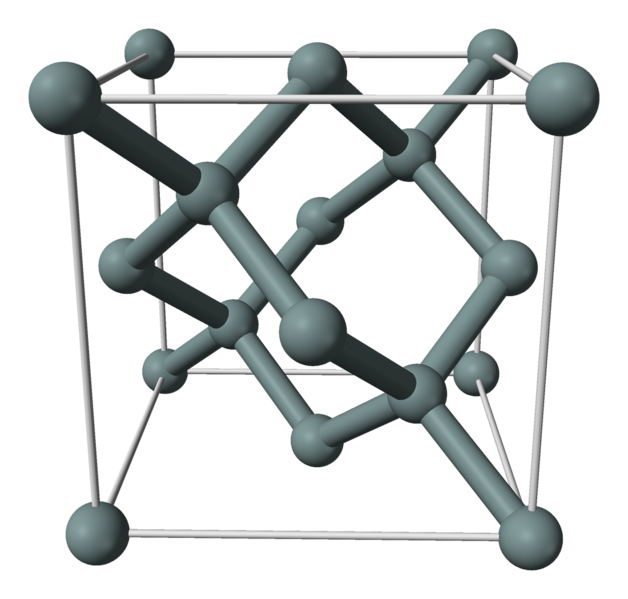
\includegraphics[scale=0.15]{figures/double_fc.png}
\caption{La maille élémentaire du cristal de silicium}
\end{center}
\end{figure}

Ses propriétés physico-chimiques en font un semi-conducteur : sa conductivité électrique est notamment bien inférieure à celle d'un métal. Dans le double réseau, chaque atome de silicium peut être considéré comme au centre d'un tétraèdre, chacun des atomes auquel il est lié se trouvant sur un des quatre sommets du tétraèdre. Les liaisons covalentes sont très solides et permettent la formation d'un cristal parfait. Tous les électrons étant utilisés dans les liaisons, aucun n'est disponible pour permettre le passage d'un courant électrique, du moins aux températures très basses ; le cristal présente une résistivité assez élevée. Lorsque la température s'élève, sous l'effet de l'agitation thermique, des électrons réussissent à s'échapper et participent à la conduction. Ce sont les électrons situés sur la couche la plus éloignée du noyau qui s'impliquent dans les liaisons covalentes. Dans le cristal, ces électrons se situent sur des niveaux d'énergie appelée bande de valence. Les électrons qui peuvent participer à la conduction possèdent des niveaux d'énergie appartenant à la bande de conduction. Entre la bande de valence et la bande de conduction peut se situer une bande interdite. Pour franchir cette bande interdite l'électron doit acquérir de l'énergie (thermique, photon...). Pour les isolants la bande interdite est quasi infranchissable, pour les conducteurs elle est inexistante. Les semi-conducteurs ont une bande interdite assez étroite.\\

\begin{figure}[htb]
\begin{center}
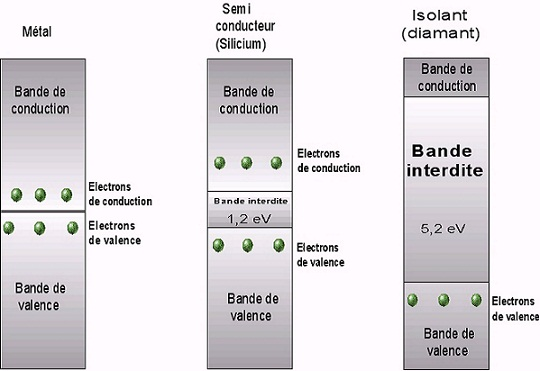
\includegraphics[scale=1.3]{figures/bande-interdite-valence-et-conduction-copie.png}
\caption{Bande de valence et de conduction de différents types de matériaux}
\end{center}
\end{figure}

L'atome qui a perdu un électron devient un ion positif et le trou ainsi formé peut participer à la formation d'un courant électrique en se déplaçant.
Dans un cristal pur, à température ordinaire, les électrons libres sont malgré tout extrêmement rares - de l'ordre de 3 pour $10^{13}$ atomes !
Si l'électron libre est capté par un atome, il y a recombinaison. Pour une température donnée ionisation et recombinaison s'équilibrent ; la résistivité diminue quand la température augmente.
Un semi-conducteur dont la conductivité ne doit rien à des impuretés est dit {\it intrinsèque}.\\

Lors de la formation du cristal de silicium il suffit d'introduire une infime quantité d'impuretés sous la forme d'atomes d'aluminium (possédant seulement 3 électrons sur leur couche externe) pour que le nombre de trous dans le cristal augmente considérablement. Le cristal est dit dopé et comme les porteurs de charges majoritaires sont des trous, positifs, le cristal est dit dopé P. Les électrons libres qui correspondent à la conductivité intrinsèque sont
appelés porteurs minoritaires.
Si un électron est arraché d'un atome voisin et vient combler le trou, tout se passe comme si c'était le trou qui s'était déplacé.
On peut également doper le cristal avec des impuretés pentavalentes (atomes possédant 5 électrons sur leur couche externe),
comme l'arsenic ou l'antimoine. On se retrouve alors avec un électron supplémentaire, donc libre. Les porteurs de charges majoritaires
sont alors de polarité négative, le cristal est dit dopé N. Les porteurs de charge minoritaires sont dans ce cas les trous (positifs)
de la conductivité intrinsèque.\\

\begin{figure}[htb]
\begin{center}
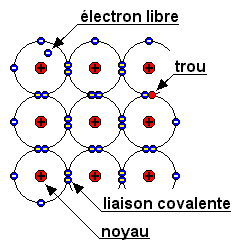
\includegraphics[scale=0.5]{figures/cristal.png}
\caption{Présence des différents porteurs de charge}
\end{center}
\end{figure}

Un atome pentavalent comme l'arsenic possède 5 électrons sur sa couche externe. En tant qu'impureté dans un cristal de silicium
(tétravalent) il fournit un électron au cristal. Il est dit atome donneur.
Si l'impureté est un atome trivalent (3 électrons sur sa couche externe, comme le bore ou l'indium) il est dit atome accepteur car il va
capter un électron et générer un trou. Les porteurs majoritaires sont beaucoup plus nombreux que les porteurs minoritaires ($10^6$ à $10^{12}$ fois
plus nombreux).\\

\paragraph{En résumé} Le fait d'introduire en très faible quantité des impuretés (opération appelée dopage) dans un cristal de semi-conducteur améliore
fortement la conductivité du cristal. Si un cristal de germanium ou de silicium a reçu des impuretés pentavalentes (arsenic, phosphore,
antimoine) il devient un semi-conducteur à conductivité N (ex: silicium N).
Un cristal de germanium dopé par des impuretés trivalentes (indium, gallium, bore) devient un semi-conducteur P.

\section{Jonction PN}
Une jonction entre des cristaux de silicium de type {\it p} et de type {\it n} est appelé une {\bf diode}. Cette jonction est le simple rapprochement
de ces deux cristaux. Ses propriétés sont particulièrement remarquables.\\

\begin{figure}[htb]
  \begin{center}
    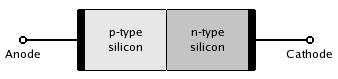
\includegraphics[scale=0.6]{figures/PN_Junction_Open_Circuited.png}
    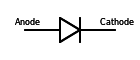
\includegraphics[scale=0.8]{figures/Diode_symbol.png}
    \caption{Jonction PN ou diode}
  \end{center}
\end{figure}

\begin{itemize}
  \item Lorsque la tension sur le semi-conducteur de type p, appelée anode, est supérieure à celle la tension sur la partie dope n (cathode), la diode est polarisée en direct et le courant circule.
  \item Lorsque la tension d'anode est inférieure ou égale à la tension de cathode, la diode est polarisée en inverse et très peu de courant circule.
\end{itemize}

\begin{figure}[h!bt]
  \begin{center}
    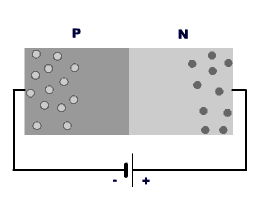
\includegraphics[scale=0.4]{figures/Diffusion3.png}
    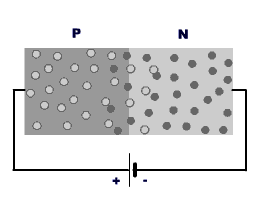
\includegraphics[scale=0.4]{figures/Diffusion4.png}
    \caption{Jonction PN passante ou bloquée en fonction de la polarisation.}
  \end{center}
\end{figure}

Ce dipôle est aussi appelé diode de redressement car il est utilisé pour réaliser les redresseurs qui permettent de transformer le courant alternatif en courant continu.

\section{Transistor MOS}

Le transistor est un composant électronique qui a deux utilités majeures : il permet d'{\bf amplifier un courant ou une tension}, ou il peut être utilisé comme un {\bf interrupteur commandable en courant ou en tension}. Dans la suite, nous n'utiliserons que cette seconde capacité. Il existe deux catégories de transistor :
\begin{itemize}
\item les transistors bipolaires, constitués par la succession de trois zones dopées PNP ou NPN.
\item les transistors MOS, qui représentent désormais plus de 85\% du marché.
\end{itemize}


%% \begin{figure}[htb]
%% \begin{center}
%% 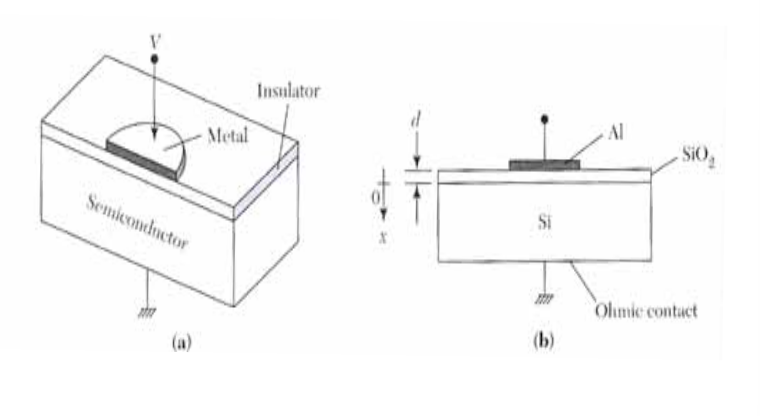
\includegraphics[scale=0.3]{figures/MOS.png}
%% \caption{Structure MOS}
%% \end{center}
%% \end{figure}

%http://www.etudes.ecp.fr/physique/illustrations/jonction_PN.htm#debut

La figure suivante présente la structure d'un tel transistor, ici de type $n$.

\begin{figure}[htb]
\begin{center}
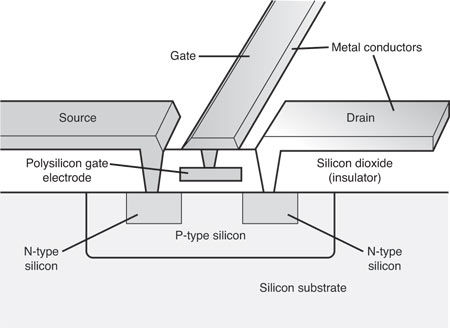
\includegraphics[scale=0.6]{figures/n-MOS_2.png}
\caption{Transistor $n-MOS$}
\end{center}
\end{figure}

Un tel transistor présente une structure en sandwich :
\begin{itemize}
\item une grille (gate) conductrice (généralement du métal ou du silicium polycristallin)
\item une couche isolante (oxyde de silicium $SiO_2$)
\item le substrat de silicium, dont la tension est généralement à la masse.
\item deux zones dopées de manière identique (ici dopées $n$), appelées source et drain.
\end{itemize}

Ces structures sont fabriquées en utilisant une série d'étapes de traitements chimiques impliquant l'oxydation
du silicium, introduction sélective de dopants (impuretés), le dépôt et la gravure de fils métalliques
et des contacts. Tout ceci à l'échelle nanométrique...La complexité de ces traitements justifie le coût très élevé des usines ({\it fab} ou {\it fonderie}) liées à
l'industrie du semiconducteur. L'entreprise taiwanannaise TSMC, leader mondial, a annoncé en 2017 que le coût de son usine permettant des gravures
à 3 nanomètres lui coûterait plus de 20 milliards de dollars. Sa capitalisation boursière était de 173 milliards de dollars fin 2018
\footnote{Chiffre qui dépasse celui d'Intel, mais reste loin de celui de Facebook (500 Milliards) ! Toutefois, pouquoi comparer ce qui n'est guère
comparable : TSMC fait partie d'une industrie "lourde" et stable. Pour mémoire,
Facebook a perdu 114 Milliards de dollars dans la seule journée du 26 juillet 2018, soit 20\% de sa valeur boursière.}.

Comme on peut l'observer, un transistor $n-MOS$ est construit à partir d'un substrat $p$ et de deux régions dopées de type $n$ (c'est l'inverse pour un transistor de type $p$). La grille permet de  contrôler le courant qui circuit entre la source et le drain. Dans le cas d'un nMOS, le substrat est à la masse : par conséquent les jonctions p-n entre les source-substrat et drain-substrat sont polarisées en inverse. Si la grille est également à la masse, aucun courant ne circule entre les deux jonctions : le transistor est non-passant, ou fermé, ou ``OFF''.

Si on élève la tension de la grille, un champ électrique se crée, qui attire les électrons libres sous la couche isolante. Si cette tension est suffisamment élevée le nombre d'électrons dépasse le nombre de trous : une région, appelée ``canal'' se crée, qui se comporte comme un semiconducteur de type $n$, alors que le substrat initial est $p$ ! Un chemin s'établit pour les électrons entre la source et le drain : le transistor devient passant. Il est ouvert ou ``ON''. Pour les pMOS, la situation est exactement opposée.\\

La tension ``suffisante'' est appelée VDD et représente la valeur logique $1$ dans les circuits numériques. Dans les années 70 et 80, VDD valait traditionnellement $5$ volts.
Plus récemment, les transistors ne pouvant supporter de telles tensions, VDD a été réduit à $3.3V$, puis $1.8V$ etc...La tension appelée VSS (ou ground) représente quant à elle la valeur logique $0$. Elle vaut normalement $0$ volts.\\

En simplifiant le mécanisme à l'extrême, les transistors MOS peuvent être vus comme des interrupteurs ON-OFF.
Lorsque la grille d'un transistor nMOS est 1, le transistor est OFF et il existe un chemin de conduction entre source et drain.
Lorsque la grille est à 0, le transistor est OFF et pratiquement aucun courant ne circule entre la source et le drain.
Le transistor pMOS fonctionne à l'opposé, étant ON lorsque la grille est à 0 et OFF lorsque la tension de grille est 1.

\begin{figure}[htb]
\begin{center}
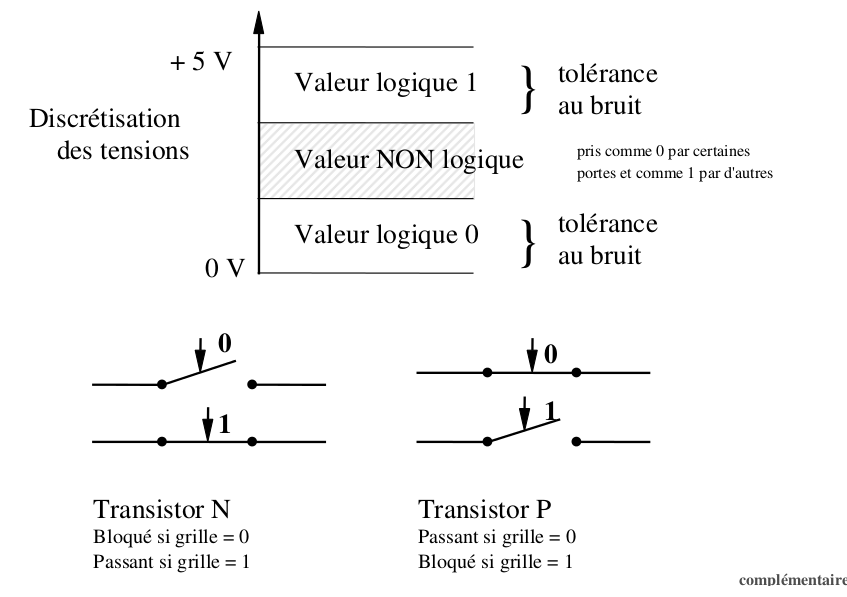
\includegraphics[scale=0.4]{figures/complementaire_1.png}
\caption{CMOS}
\end{center}
\end{figure}

\section{MOS complémentaires}

\paragraph{Principe}
Nous sommes désormais dotés de deux types de transistors. Technologiquement, il a longtemps été question de ne réaliser les circuits numériques à l'aide d'un seul type de transistor (N {\bf ou} P). Mais la technique qui sort largement vainqueur est la logique complémentaire CMOS. Elle consiste à utiliser de manière duale les transistors P {\bf et} N, dans le but de réaliser une fonction logique. Les transistors P sont utilisés pour tirer à 1 et les transistors N pour tirer à 0. Il n'y a pas de perte de seuil. Pour associer ces deux types de transistors, les techniques de dépôts micro-électroniques deviennent plus complexes : il faudrait être à même de
présenter deux substrats différents : un substrat P "collé"" à un substrat N ! Ce n'est pas ce qui est fait technologiquement : en réalité,
on réalise plutôt une zone N sur un substrat P, comme représenté sur la figure \ref{cmos1}.

\begin{figure}[htb]
\begin{center}
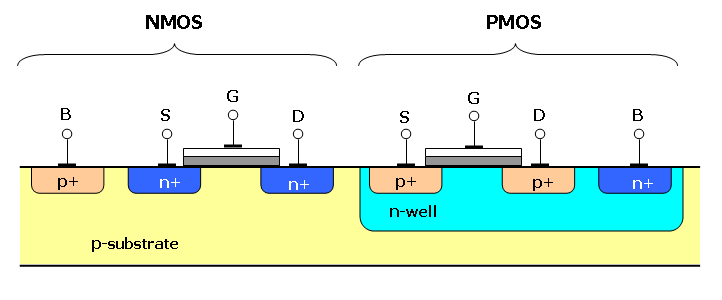
\includegraphics[scale=0.4]{figures/Cmos_impurity_profile.PNG}
\caption{Transistor $C-MOS$}
\label{cmos1}
\end{center}
\end{figure}

\paragraph{Inverseur CMOS}

A titre de premier exemple, considérons le cas d'un {\it inverseur} CMOS sur la figure \ref{cmos2}. On voit qu'il est constitué de deux transistors : la source du transistor P est l'alimentation (5 volts ici),  tandis que celle
du transistor N est la masse (0 V). Ils sont assemblés par leur drain commun et commandés par une entrée (gate) commune.
Lorsque la tension appliquée à l'entrée vaut 0, le transistor P est passant, tandis que le transistor
N est bloqué : la tension issue de l'alimentation se retrouve en sortie. C'est ainsi que l'on a inversé le 0 en 1.
L'inverse s'applique dans le cas d'une tension d'entrée égale à 5 Volts : on transforme le 1 en 0.

\begin{figure}[htb]
  \begin{center}
    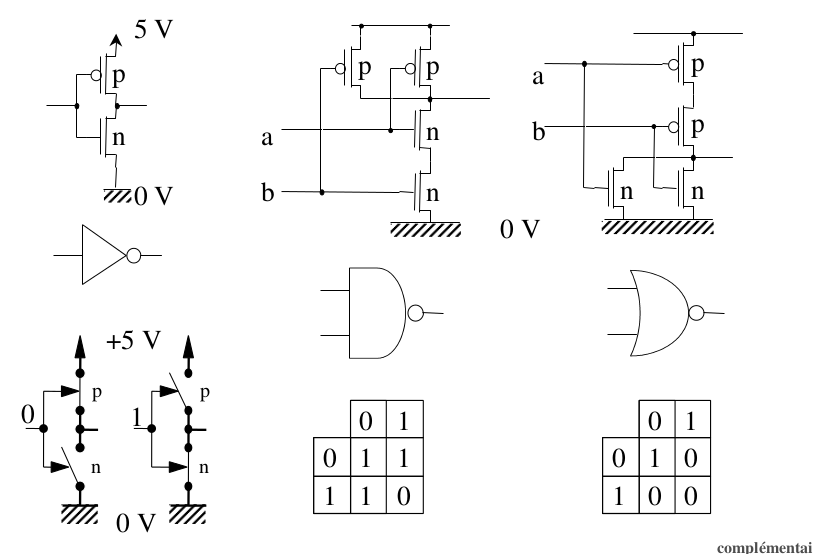
\includegraphics[scale=0.4]{figures/complementaire_2.png}
    \caption{Inverseur logique, porte Nand2 et Nor2 en technologie CMOS}
    \label{cmos2}
  \end{center}
\end{figure}

\paragraph{Principe de dualité}

C'est donc par un montage judicieux, rassemblant deux transistors dopés différemment, que se réalise la fonction d'inversion logique.
La même figure \ref{cmos2} montre que cet assemblage peut se généraliser en réalisant {\it deux réseaux duaux} de transistors P et N.
Par exemple, une porte logique NAND, à deux entrées, se réalise en mettant deux transistors P en {\it parallèle}, alors que les transistors N sont en {\it série}.
Cett dualité se généralise à toutes les fonctions logiques complexes (fig \ref{cmos3}).

\begin{figure}[htb]
  \begin{center}
    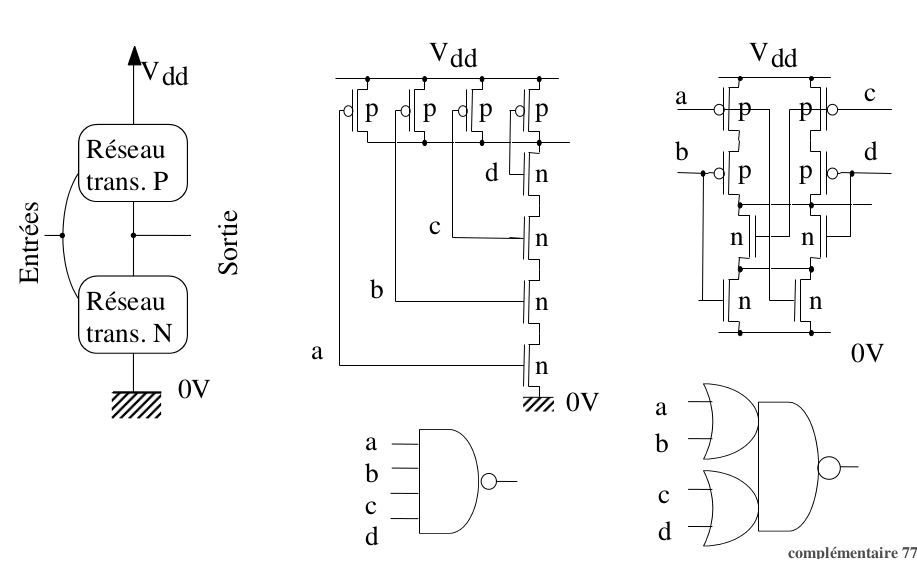
\includegraphics[scale=0.4]{figures/complementaires_2.png}
    \caption{Principe de dualité des réseaux P et N pour des portes logiques complexes}
    \label{cmos3}
  \end{center}
\end{figure}

\section{Niveaux d'abstraction}

\paragraph{De la porte logique au masque métré}
\begin{figure}[htb]
  \begin{center}
    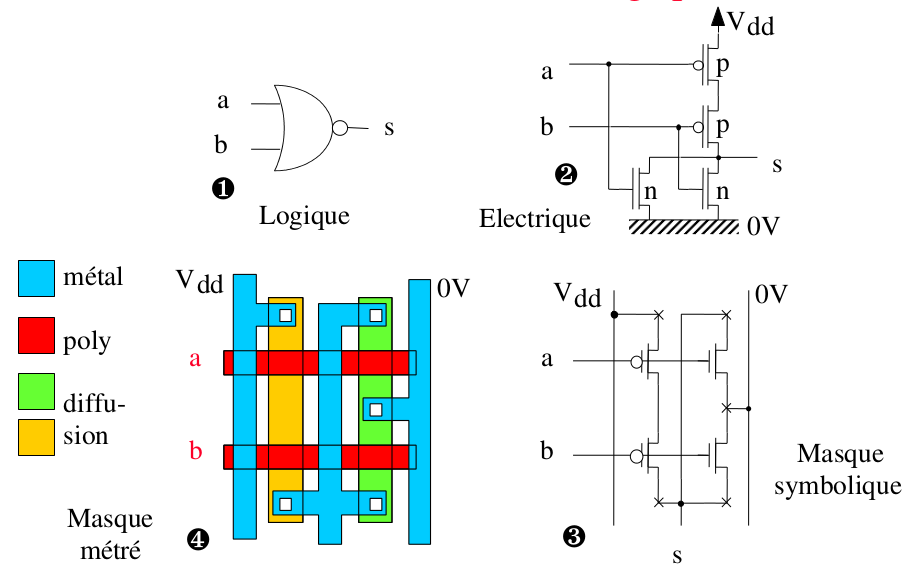
\includegraphics[scale=0.4]{figures/vues_4.png}
    \caption{De la port logique Nor2 au masque métré}
  \label{vues}
  \end{center}
\end{figure}

La montée en abstraction suggérée jusqu'ici, nous faisant passer du silicium à des transistors, puis des premières portes logiques, est illustrée sur la figure \ref{vues}, {\it à rebours} :
le microélectronicien qui souhaite une porte logique (ici un NOR2) devra passer par :
\begin{enumerate}
  \item une décomposition en réseaux P et N de transistors "abstraits", c'est-à-dire affranchis de toute contrainte physique de réalisation. C'est une  sorte de "plan" d'architecte.
  \item un masque symbolique, où l'on dispose soigneusement les équipotentielles de manière géométrique.
  \item un masque métré, où la nature physique des équipotentielles est indiquée (métal, polysilicium etc), ainsi que leur métrage exact. Ce métrage doit respecter des contraintes de {\it layout} (disposition)
  physique précis : certaines zones doivent ne pas s'approcher trop près d'autres région etc...
\end{enumerate}

Ce dernier masque métré reste dessiné dans le plan. Charge à des ordinateurs de calculer leurs dispositions exactes en trois dimensions...Le schéma \ref{cmos4} expose la complexité de
l'enchevêtrement de ces canaux, pour quelques transistors seulement...

\begin{figure}[htb]
  \begin{center}
    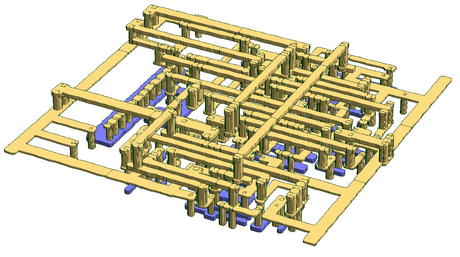
\includegraphics[scale=0.4]{figures/enchevetrement.png}
    \caption{Représentation 3D d'un assemblage de transistors en microélectronique (substrat unique)}
    \label{cmos4}
  \end{center}
\end{figure}

\paragraph{De la porte logique vers le système embarqué}

En 1983, Gajski et Kuhn ont proposé un schéma \ref{gajski} résumant les différentes abstractions d'un système embarqué. Il se présente comme un "Y", dont les trois axes sont :
\begin{itemize}
  \item le comportement du système, vu à différents niveaux d'abstractions
  \item la structure du système, vue à différents niveaux d'abstractions
  \item la géométrie du système, vu à différents niveaux d'abstractions
\end{itemize}

\begin{figure}[htb]
  \begin{center}
  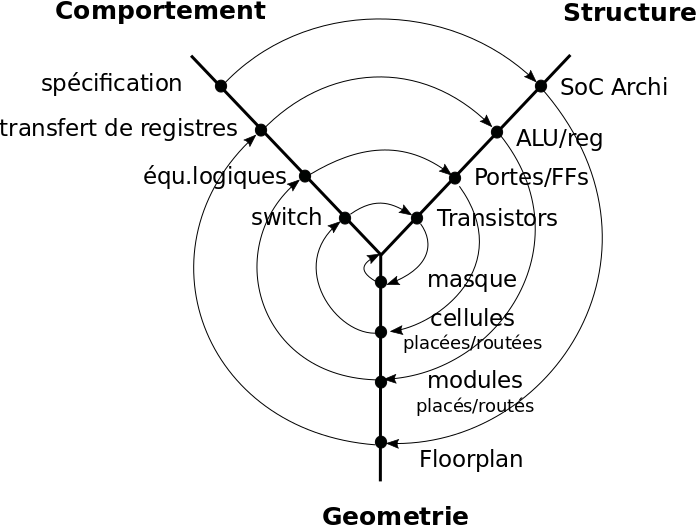
\includegraphics[scale=0.4]{figures/ychart.png}
  \caption{"Y" de Gajski-Kuhn (1983)}
  \label{gajski}
  \end{center}
\end{figure}

La conception d'un "système sur puce" est représenté comme la
succession d'activités d'ingénierie, qui font systèmatiquement passer d'un niveau comportemental à une structure, puis à un niveau géométrie.
Cette succession se répéte en spirale, jsqu'à aboutir à un système réalisé.

Au final, on pourra se satisfaire du schéma \ref{abstractions} qui illustre un sous-ensemble de ces abstractions d'un système.

\begin{figure}[htb]
\begin{center}
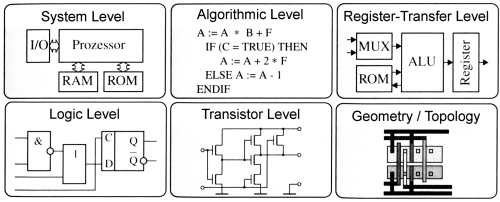
\includegraphics[scale=0.4]{figures/abstractions.png}
\caption{Six vues différentes d'une même système numérique}
\label{abstractions}
\end{center}
\end{figure}

%\section{Equations du transistor MOS en petit signal}

%\section{Technologies microélectroniques}
\section{Numérique versus Analogique}

Nous avons passé sous silence et tenu pour acquis les avantages des circuits numériques sur les circuit analogiques. Ces derniers
ne sont désormais plus utilisés qu'aux interfaces d'un système numérique : pour capter des signaux physiques, pour les amplifier ou les débruiter, etc.
L'Electronique analogique garde tout son intérêt dans le domaine des capteurs, au plus proche de ce monde physique. Mais l'essentiel des traitements effectués
sur le signal se fait par la suite dans un système totalement numérique. En dehors des traitements dédiés, la notion d'ordinateur analogique a totalement disparue, au profit
des ordinateurs que l'on connait depuis longtemps.

La suprémacie du numérique sur l'analogique provient principalement de sa précision maîtrisée : tous les traitements donnent des valeurs exactes, avec une fidélité absolue.

La figure \ref{comparaison} liste quelques uns des avantages et inconvénients des deux Electroniques.

  \begin{figure}[htb]
    \begin{center}
    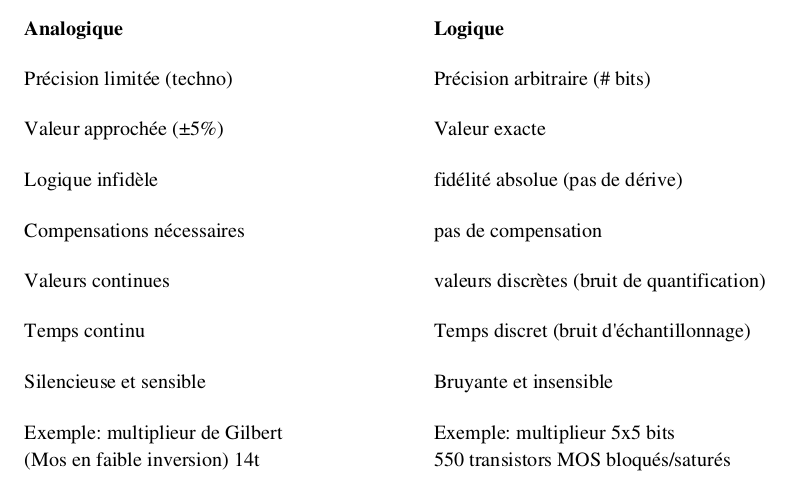
\includegraphics[scale=0.4]{figures/avantages.png}
    \caption{Electronique Analogique et Numériques comparées}
    \label{comparaison}
    \end{center}
  \end{figure}

\section{Conclusions}

Ce chapitre se veut court, car l'ENSTA-Bretagne n'entend pas former des spécialistes de la micro-électronique, ni de la nano-électronique.
Je vous invite toutefois à ne pas perdre de vue, à travers vos lectures, les avancées probables dans le domaine : les progrès de la physique théorique
et appliquée nous apporterons très certainement des révolutions à la hauteur de celles que nous avons vécu dans les années 70. A titre d'exemple, en 2017,
l'ordinateur quantique est en vue ! les promesses seront-elles tenues ?
On peut de même inciter à garder un oeil critique sur les techniques numériques : le tableau suivant compare les avantages et inconvénients de l'électronique
analogique et numérique : comme on peut le voir le numérique se révèle bourré de défauts (exemple : il est plus compliqué de réaliser des opérations arithmétiques,
il est très bruyant,...).

\chapter{Représentations numériques}

\minitoc

\section{Notion de bases ou radix}

\subsection{Décomposition en puissance de la base}
Les nombres que nous manipulons tous les jours s'expriment en base (ou {\it radix}) $10$.
On parle de base $10$ car on utilise $10$ symboles (appelés {\it chiffres}) allant de $0$ à $9$ inclus.
Par la suite, on s'autorisera à parler de $digits$.
Dans un nombre, ces digits sont en fait des {\it coefficients} du système décimal :
pour former un nombre, on multiplie ces coefficients par les puissances successives de $10$.
Par exemple le nombre $142$ s'exprime ainsi :

$$ 142 = 1\times 10^2 + 4\times 10^1 + 2\times 10^0$$

Il en est de même des nombres fractionnaires comme :
$$ 142.34 = 1\times 10^2 + 4\times 10^1 + 2\times 10^0 + 3\times 10^{-1} + 4\times 10^{-2}$$

La formule générale pour la base $10$ est bien entendu :
$$ x = \sum_{i=-\infty}^{i=\infty} c_i.10^i, \mbox{avec } c_i \in \{0\dots 9\}$$
et se généralise pour toute base $r$ :
$$ x = \sum_{i=-\infty}^{i=\infty} c_i.r^i, \mbox{avec } c_i \in \{0\dots (r-1)\} $$

Les ordinateurs n'utilisent pas la base $10$, mais la base $2$, qui ne possède que deux valeurs de
coefficients possibles : $0$ et $1$. De plus, ces ordinateurs ne peuvent stocker un nombre infini de digits et devront passer par
une représentation des nombres avec un nombre fini de digits

Afin d'éviter toute confusion par la suite, nous plaçons en indice du nombre l'indication de la base utilisée,
ce qui évitera de nous perdre lors des changements de base. Par exemple, on peut noter :
$$10110_{10} = 10011101111110_2$$

En pratique, il existe deux autres bases indispensables aux informaticiens et électroniciens : la base octale (base 8) et la base
hexadécimale (base 16). La première n'utilise que les digits allant de $0$ à $7$. En hexadécimal, on doit introduire
de nouveaux symboles au delà du $9$ : on utilise --dans l'ordre-- les lettres (majuscules ou minuscules) A, B, C, D,
E et F, correspondant respectivement à 10,11,12,13,14 et 15. La table suivante montre les 18 premiers nombres dans
le système décimal, binaire, octal et hexadécimal, ainsi que deux autres représentations sur lesquelles nous
reviendrons un peu plus tard).\\

\begin{table}
 \centering
  \begin{tabular}{ | r | r | r | r | r | r |}
    \hline
    \multicolumn{6}{|c|}{base (ou nom du code)} \\
    \hline
    10 & 2 & 8 & 16 & BCD & Gray \\ \hline \hline
   0 &     0 &     0 &     0 &  0000 &     0 \\ \hline
   1 &     1 &     1 &     1 &  0001 &     1 \\ \hline
   2 &    10 &     2 &     2 &  0010 &    11 \\ \hline
   3 &    11 &     3 &     3 &  0011 &    10 \\ \hline
   4 &   100 &     4 &     4 &  0100 &   110 \\ \hline
   5 &   101 &     5 &     5 &  0101 &   111 \\ \hline
   6 &   110 &     6 &     6 &  0110 &   101 \\ \hline
   7 &   111 &     7 &     7 &  0111 &   100 \\ \hline
   8 &  1000 &    10 &     8 &  1000 &  1100 \\ \hline
   9 &  1001 &    11 &     9 &  1001 &  1101 \\ \hline
  10 &  1010 &    12 &     a & 00010000 &  1111 \\ \hline
  11 &  1011 &    13 &     b & 00010001 &  1110 \\ \hline
  12 &  1100 &    14 &     c & 00010010 &  1010 \\ \hline
  13 &  1101 &    15 &     d & 00010011 &  1011 \\ \hline
  14 &  1110 &    16 &     e & 00010100 &  1001 \\ \hline
  15 &  1111 &    17 &     f & 00010101 &  1000 \\ \hline
  16 & 10000 &    20 &    10 & 00010110 & 11000 \\ \hline
  17 & 10001 &    21 &    11 & 00010111 & 11001 \\ \hline
  \end{tabular}
  \caption{Table des correspondances entre bases $10$, $2$, $8$, $16$, puis code BCD et code de Gray}
\end{table}

Enfin, notons qu'il existe des bases plus exotiques. Par exemple, la numération mésopotamienne (utlisée par babyloniens notamment),
a recours à la base 60 : c'est la base sexagésimale. Elle date d'environ 3000 ans avant notre ère ! On en retrouve quelques vestiges dans notre système horaire et dans la mesure des angles.
A titre de curiosité, la figure \ref{sexa} présente une pierre datant du \siecle{17} siècle avant Jésus-Christ.
Elle démontre la maîtrise du calcul de $\sqrt 2$, dans cette base sexagésimale : les archéologues nous enseignent que cette tablette
vise à établir l'égalité suivante, calculée il y a près de 38 siècles !
$$\sqrt 2 \approx 1.414212=1+\frac{24}{60}+\frac{51}{60^2}+\frac{10}{60^3}=\frac{30547}{21600}$$
\begin{figure}[htb]
  \begin{center}
    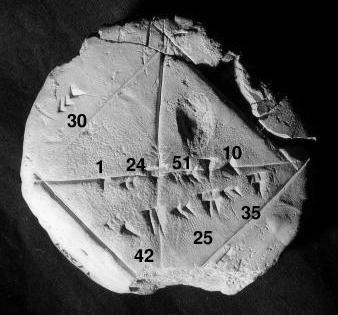
\includegraphics[width=4cm]{./figures/Ybc7289-bw.jpg}
    \caption{(Wikipedia) Tablette avec l'écriture en numération sexagésimale de 1/2 et des valeurs approchées au six dix-millionièmes de $\sqrt 2$, ainsi que :
    $\frac{\sqrt 2}{2}=42+\frac{20}{60}+\frac{35}{60^2}+\frac{35}{60^2}=\frac{30547}{720}$}
    \label{sexa}
  \end{center}
\end{figure}

\paragraph{Nombre de bits nécessaires pour représenter un entier $x$}
On déduit aisément le nombre de bits $n$ nécessaires à la représentation d'un entier $x$ :
pour $n$ bits, on a $x \leq 2^n-1 < 2^n$, d'où $log_2(x)<n$.
Avec $n\in \mathbb(N)$, on déduit \fbox{$n=\floor*{log_2(x)}+1$}, où $\floor*{\alpha}$ représente le plus petit entier inférieur à $\alpha$.

\paragraph{Erreur de calcul liés aux représentations}
Nous verrons très bientôt que les ordinateurs sont capables d'effectuer les calculs traditionnels de l'arithmétique, au sein d'une Unité Arithmétique et Logique (UAL).
Le nombre de bits des opérandes en entrée de cette UAL sont limités (8,16, 32 voire 64 bits). Les calculs réalisés {\it directement} (matériellement) par les ordinateurs seront
forcément entachés d'erreurs liées à ces limitations, dont l'ingénieur devra se méfier. Notons toutefois que tous les langages possèdent des bibliothèques qui permettent
d'augmenter le nombre de digits manipulés de manière logicielle, avec un surcoût important en terme de temps de calcul :
il s'agit de l'arithmétique "multi-précision" plus communément appelée {\it arbitrary-precision arithmetic} ou {\it bignum}.
Les temps de
calculs en bignum conduit la plupart des scientifiques à ne pas les utiliser et à se limiter au calcul fourni directement par la machine..

\subsection{Conversion entre bases}
Grâce aux formules précédentes, nous savons transformer un nombre exprimé dans une base {\it r} en en nombre décimal.
Il est à présent important de savoir faire l'inverse, à savoir : convertir un nombre décimal $x_{10}$ vers tout autre base {\it r} .
Ceci peut se faire de manière mécanique : il suffit de diviser le nombre $x$ (dividende) par $r$ (diviseur), puis de répéter
l'opération sur le quotient jusqu'à ce que ce quotient soit nul. Le premier reste obtenu sera le digit
le plus à droite (En base  binaire, on parle de LSB : least significant bit), et le dernier reste  le digit le plus à gauche
(MSB : most significant bit).

Dans le cas de nombres fractionnaires, il faut procéder de la manière suivante : multiplier le nombre par $r$ jusqu'à obtenir
un nombre sans partie fractionnaire. Ceci n'est évidemment pas toujours possible : selon les nombres en présence, ce calcul ne conduit pas
forcément à un nombre sans partie fractionnaire ! Notamment, il arrive fréquemment que des nombres, exprimables avec un nombre fini de digits dans une base,
puissent nécessiter un nombre {\it infini} de digits dans une autre base.

\subsection{Exemples}
\begin{itemize}
\item {\bf Convertir le nombre $12_{10}$ en binaire}\\
\underline{Solution:}\\
\begin{align*}
 12 / 2 &= 6 + 0 \\
  6 / 2 &= 3 + 0 \\
  3 /2  &= 1 + 1 \\
  1 / 2 &= 0 + 1
\end{align*}

Par conséquent :
$( 12 )_{10} = ( 1100 )_2$\\

\item {\bf Convertir $( 0.75)_{10}$ en binaire}\\
\underline{Solution:}\\
\begin{align*}
0.75 \times 2 &= 1.5 = 1 + 0.50 \\
0.50 \times 2 &= 1.0 = 1 + 0 \\
\end{align*}
Ainsi : $$( 0.75)_{10} = ( 0.11)_{2}$$\\

\item {\bf Convertir $( 0.39654 )_{10}$ en binaire}\\
\underline{Solution:}\\
\begin{align*}
0.39654 \times 2 &= 0.79308 = 0 + 0.79308 \\
0.79308 \times 2 &= 1.58616 = 1 + 0.58616 \\
0.58616 \times 2 &= 1.17232 = 1 + 0.17232 \\
0.17232 \times 2 &= 0.34464 = 0 + 0.34464 \\
\end{align*}
etc...Cette conversion n'a pas de fin. La partie fractionnaire ne peut s'exprimer sous la forme d'une somme exacte de puissance de $2$. On notera la solution :
$$( 0.39654 )_10 = ( 0.0110... )_2$$
\end{itemize}

Il est important que vous sachiez rapidement effectuer ces conversions avec votre ordinateur ou calculatrice préférée
\footnote{Pour votre information, il est possible d'utiliser Google pour effectuer cela : tapez ``0x123 in octal'' dans l'invite de Google...Vous obtenez $0o443$}.

\subsection{Conversions binaire, hexadécimal, octal}
Comme $2^4=16$, il s'en suit que la représentation binaire de chaque digit de la base $16$ nécessite $4$ bits. Pour la base octale, il en suffit de $3$.
De ce fait, les conversions de nombres binaires vers l'hexadécimal ou l'octal se réalisent simplement, par groupement de bits. En partant de la droite, il suffit par exemple de regrouper 4 bits pour obtenir un digit hexa. Par exemple :
$$\mbox{le nombre } 101101_2 = 10\_1101_2 = 0010\_1101_2=2D_{16}={\bf 0x2D}$$

Dans le cas de nombre fractionnaires, le sens de lecture s'inverse pour la partie fractionnaire. Ainsi :
$$\mbox{le nombre } 1011.01_2 = 1011.0100_2 = B.4_{16}$$

On procède de même pour la traduction octale.
$$( 10110001101011.1111 )_2 =(010\ 110\  001\  101\  011\  .\  111\  100)_2 = ( 26153.74 )_8$$

\subsection{Bits, bytes, nibbles, words}
La plus petite unité informatique est le bit, qui est l'abréviation de {\it binary digit}.
Toutefois rares sont les ordinateurs qui ne traitent qu'un seul bit à la fois : la plus petite la grandeur manipulable par la quasi-totalité des ordinateurs reste l'{\bf octet} : c'est l'aggrégation de 8 bits. Sa traduction anglaise est le {\it byte}, qui se prononce {\it bait} et qui ne doit pas être confondu avec le bit. Le regroupement de 4 bits est moins connu, mais indispensable : il s'agit du {\bf quartet} ou {\it nibble} en anglais. Nous verrons plus loin en quoi il est important. Enfin, on parle de {\bf mot} ou {\it word} pour le regroupement de 16 bits, sans toutefois que cette définition soit parfaitement admise. On parlera d'ailleurs de processeurs qui opèrent sur des mots de 16 bits, 32 bits, 64 bits etc...\\

Les bits des quartets, octets et mots sont généralement manipulés simultanément, lorsque la machine possède les circuits qui le permettent. Nous y reviendrons par la suite.

\paragraph{Première addition binaire}
Considérons le cas de l'addition binaire. Seuls 4 combinaisons sont à étudier :
\begin{align*}
0+0 &= 0 \\
0+1 &= 1 \\
1+0 &= 1 \\
1+1 &= 0 \mbox{ et une retenue de 1}
\end{align*}

Nous verrons, au chapitre suivant, comment forcer le silicium à réaliser électriquement ce calcul !






\section{Représentation des entiers négatifs.}

Jusqu'ici nous n'avons pas parlé de nombres négatifs. Comment représenter des nombres négatifs ? La manière la plus intuitive serait de considérer un nombre négatif comme la juxtaposition de deux informations représentées isolément :
le signe et la valeur absolue (``magnitude'').
Le signe pourrait n'être encodé que sur 1 seul bit : 0 ou 1 représentant par exemple le + et le - respectivement.
On appelle cette représentation "magnitude signée". Cette représentation "positionnelle" est tout à fait envisageable,
mais elle se révèle \textbf{inefficace matériellement}.
Elle oblige notamment à revoir le calcul de l'addition.
Elle a donc rapidement été abandonnée au cours de l'histoire de l'Informatique.
A l'inverse, certaines opérations sont grandement simplifiées par le recours à la \textbf{représentation complémentée} d'un nombre.
Aujourd'hui, les ordinateurs stockent les valeurs négative en binaire, en complément à 2.
Nous allons donc commencer par cette "bonne" représentation, puis nous reviendrons sur ces autres représentations obsolètes ou rares.

\subsection{Complément à $r$ d'un nombre}
Le complément à $r$ d'un entier $n$ sur $k$ digits, noté $C_{r,k}(n)$ est défini par :
$$"-n"_{r,k}=C_{r,k}(n)=r^k-n$$
Le nombre précédé de son signe négatif est écrit entre guillemet, car il ne s'agit que d'une convention "picturale" :
ce "-" n'est pas un digit de la base.\\

La formule fondamentale pour un nombre binaire se réduit donc à :

\begin{equation}
  \boxed{$$"-n"_{2,k}=C_{2,k}(n)=2^k-n$$}
\end{equation}

On a ainsi, pour un représentation de $-3$ en complément à 2, représenté sur 4 bits :
$$"-3"_{2,4}=C_{2,4}(3)=2^4-3=13=1101_2$$

On dit que 13 est le complément à 2 de 3 (et non $-3$) sur 4 bits.

\paragraph{Remarques}
\begin{enumerate}
  \item L'expression "complément à 2", fréquemment utilisée, est un raccourci langagier pour dire "complément à $2^k$" !
  \item Lorsqu'on augmente le nombre $k$ de digits autorisés dans la représentation, sa représentation change beaucoup, mais de manière structurée. Le signe se
  propage vers la gauche. En utilisant le signe "-" traditionnel, nous ne sommes pas habitués à de tels changements.
  Ainsi :
  $$"-3"_{2,5}=C_{2,5}(3)=2^5-3=29=11101_2$$
  \item Sur $k$ bits, on ne pourra représenter que les nombres $\{-2^{k-1}...+2^{k-1}-1\}$, c'est-à-dire plus de nombres négatifs que positifs.
  \item Deux applications successives de $C_{r,k}$ redonnent évidemment le nombre initial : $$C_{2,4}(C_{2,4}(3))=C_{2,4}(13)=2^4-13=3$$
\end{enumerate}



\subsection{Conversion d'une représentation binaire en complément à 2}
Soit un nombre $W$ de bits et soit $\vec{x}=[x_{w-1},x_{w-2},\dots,x_0]$ de bits. Nous avons vu précédemment (sans la nommer) que la simple fonction :
$$B2U_w(\vec{x}) \doteq \sum_{i=0}^{w-1}x_i2^i$$ définit la valeur non-signée ("unsigned") de $\vec{x}$, dans $\mathbb{N}$. Les valeurs limites de cette fonction sont :

\[
\left\{
\begin{array}{r c l}
UMax_w  &=& \sum_{i=0}^{w-1}2^i=2^w-1 \\
UMmin_w &=& \sum_{i=0}^{w-1}0=0
\end{array}
\right.
\]
On a donc : $$B2U_w : \left\{0,1 \right\}^w \rightarrow \left\{0,\dots,2^w-1\right\} $$
La fonction inverse est notée $B2U_w^{-1}$.
Elle permet de passer à un code binaire sur $w$ bits à partir d'un nombre compris entre $0$ et $2^w-1$.
Cette fonction possède la très bonne propriété de fournir un encodage unique de ce nombre entier positif.\\

De manière similaire, on définit désormais la fonction qui permet de calculer la valeur du vecteur $\vec{x}$ dans le cas d'une valeur
signée,
c'est-à-dire négative ou positive, \textbf{en complément à 2}. En notant $B2T$ la fonction "binary to two's complement", on a :

$$B2T_w(\vec{x}) \doteq -x_{w-1}2^{w-1} + \sum_{i=0}^{w-2}x_i2^i$$
Désormais, le bit de poids fort, le plus à gauche, contribue de manière négative à la somme totale.
On a ainsi : $B2T_3(101)=-1.2^2+0.2^1+1.2^0$
Calculons les valeurs min et max de cette fonction. Pour $\vec{x}=[10\dots 0]$ et $\vec{x}=[01\dots 1]$ respectivement,
on trouve \footnote{On rappelle que la formule d'une suite géométrique de raison $q$ : $$S_n=a\sum_{k=0}^{k=n} q^k= a \frac{1-q^{n+1}}{1-q} $$} :
\[
\left\{
\begin{array}{r c l}
TMin_w &=& -2^{w-1}\\
TMax_w &=& \sum_{i=0}^{w-2}2^i=2^{w-1}-1
\end{array}
\right.
\]

On a donc : $$B2U_w : \left\{0,1 \right\}^w \rightarrow \left\{-2^{w-1},\dots,2^{w-1}-1\right\} $$

On pourra également dénoter cette fonction $C_{2,w}(\vec{x})$.\\

Testons ces formules, dans un cas simple : $C_{2,3}$, c'est-à-dire le complément à 2 sur 3 bits.
Dans ce cas, on peut compter de $-4 \text{ à } 3$. On constate par exemple que $C_{2,3}(101_2=-3_{10})=101_2=5_{10}$

\begin{table}
 \centering
  \begin{tabular}{ | r | r || r |}
    \hline
    signé & bit vector & non-signé\\ \hline \hline
    -4    & 100        & 4        \\ \hline
    -3    & 101        & 5        \\ \hline
    -2    & 110        & 6        \\ \hline
    -1    & 111        & 7        \\ \hline
     0    & 000        & 0        \\ \hline
     1    & 001        & 1        \\ \hline
     2    & 010        & 2        \\ \hline
     3    & 011        & 3        \\ \hline
  \end{tabular}
  \caption{Entiers relatifs de $-4 \text{ à } 3$, traduits en complément à 2 sur 3 bits et conversion en entier non-signé}
\end{table}

\subsection{Astuces pour complémenter à 2}
Le complément à 1 d'un nombre binaire consite à simplement inverser tous ses bits.\\
Le complément à 2 d'un nombre binaire consiste à :
\begin{itemize}
\item laisser inchangé le 1 le plus à droite, ainsi que tous les 0 les plus à droite.
\item modifier tous les autres digits.
\end{itemize}

Il existe toute fois une autre méthode, qui se retient plus facilement (peut-être). Elle consiste en une pseudo-formule simple :

\begin{equation}
  \boxed{"-A"=\barre{A}+1}
\end{equation}

{\bf Exemple} : pour trouver le complément à deux de $1101100_2$. On inverse tous les bits et l'on additionne 1.
$$0010011 + 1 = 0010100$$

\subsection{A propos du "bit de signe"}

L'expression "bit de signe" est quelque peu ambigue. Cherchons à faire croître le nombre de bits dans la représentation d'un nombre négatif (disons -5).
Un petit calcul mène aux résultats consignés dans la table \ref{position_bit_signe}.
\begin{table}
 \centering
  \begin{tabular}{ | r | r |}
    \hline
    $C_{2,4}(-5)$ & 1011 \\ \hline
    $C_{2,5}(-5)$ & 11011 \\ \hline
    $C_{2,6}(-5)$ & 111011 \\ \hline
    $C_{2,7}(-5)$ & 1111011 \\ \hline
  \end{tabular}
  \caption{Position du bit de signe pour un nombre de bits croissant : le bit se "propage" à gauche)}
  \label{position_bit_signe}
\end{table}
On s'aperçoit que le bit le plus à gauche (MSB) se propage vers la gauche, jusqu'au MSB.
Notons ainsi qu'il pas exact de dire que le bit de signe se situe {\it seulement} en MSB : nos exemples
montrent bien que le "caractère négatif" d'un nombre peut apparaître, selon la valeur $w$, bien avant le MSB.
Toutefois, on doit retenir que c'est le bit MSB qui permet, d'un seul coup
d'oeil, de discriminer les valeurs positives des valeurs négatives.
Dans cette représentation, le bit en position $n-1$ est le bit dit ``de signe'' : il doit être vu que comme un indicateur sur le signe du nombre représenté
(1 signifie '-' et 0 signifie '+'), mais les autres bits ne représentent pas directement $|n|$...

\subsection{Conversion d'un nombre signé vers un nombre non signé}
Parmi les allers-retours entre représentations des nombres, il est fréquent de chercher à convertir un nombre signé en nombre non-signé. Dans ce cas, on a :
$\forall x \in \mathbb{Z}_w / TMin_w \leq x \leq TMax_w:$

\[TU_w(x) = \left\{
\begin{array}{l l}
  x+2^w & \quad \text{si $x < 0$} \\
  x     & \quad \text{si $x >= 0$}\\ \end{array} \right. \]


\section{Représentations alternatives, obsolètes ou rares}

\subsection{Représentation en Magnitude signée}
La représentation en magnitude signée est simplement :
$$B2S_w(\vec{x}) \doteq (-1)^{x_{w-1}} \sum_{i=0}^{w-2}x_i2^i$$

\subsection{Représentation en complément à 1}
Il existe également une représentation des nombres en complément à 1, très légèrement différente du complément à 2.
$$B2T_w(\vec{x}) \doteq -x_{w-1}(2^{w-1}-1) + \sum_{i=0}^{w-2}x_i2^i$$

Ces deux représentations ont la curieuse (et facheuse) propriété de proposer (chacune) deux représentations du 0 : soit en tant que $+0$, soit en tant que
$-0$. On imagine aisément que, bien que ces représentations soient différentes, il faudrait, au final, que les calculateurs numériques les traitent comme bien évidemment égales.
Ces "cas" à distinguer sont à l'origine de l'abandon de ces représentations, dans les systèmes numériques.

%==================================================================================================================
\subsection{Code BCD et code de Gray pour les entiers non-signés}

Nous avons parlé des représentations des entiers dans différentes bases. Lorsque le nombre total d'entiers à encoder est connu, on peut également chercher à représenter ces entiers par d'autres encodages ou {\it système de numération}. Cela est très fréquent dans les ordinateurs, car les architectures sont par nature finie en dimension. Hors de question de compter à l'infini ! Il existe de nombreux encodages, du plus simple ou plus compliqué. Par exemple, certains codages prédisposent à la simplification de la détection et même la correction d'erreur lors d'une communication numérique (portable, TV numérique,...) ! Nous ne pouvons nous attarder sur tous ces codages, mais sachez que c'est en fait une discipline à part entière, avec ses problématiques et enjeux propres.

\subsubsection{Code BCD}
Le codage BCD singifie ``binary coded decimal''. Chaque digit décimal $0$ à $9$ est alors traduit directement par 4 bits. Ceci est évidemment assez naturel.
\begin{center}
\begin{tabular}{|cc|cc|}
\hline
Chiffre & Quartet & Chiffre & Quartet \\
\hline
0   & 0000 &       5  &  0101 \\
1   & 0001 &       6  &  0110 \\
2   & 0010 &       7  &  0111 \\
3   & 0011 &       8  &  1000 \\
4   & 0100 &       9  &  1001 \\
\hline
\end{tabular}
\end{center}

Pour coder un nombre tel 147 il suffit de coder chacun des chiffres 1, 4 et 7 ce qui donne 0001, 0100, 0111. Cette représentation a un intérêt pratique certain : lorsqu'on réalise un appareil qui affiche des valeurs entières de plusieurs digits, le code BCD permet d'isoler l'électronique de chaque digit, de manière triviale.

\subsubsection{Code de Gray}
Souvenons nous par exemple que le passage de 7 à 8 en binaire classique fait commuter 4 bits : tous les bits changent de valeurs ! Le code de Gray (aussi appelé {\it codage binaire réfléchi}) vise à éviter de telles commutations simultanées : il est constitué d'une manière telle que {\it seul 1 digit binaire change entre un entier $n$ et son successeur $n+1$}. En pratique, cela évite de commuter un grand nombre de dispositifs en même temps, lors d'un comptage régulier. Le codage de gray fait partie d'un ensemble de codes appelés à ``distance minimale''.

\begin{center}
\begin{tabular}{|c|c|c|}
\hline
décimal & binaire classique & Gray \\
\hline
 0 & 0000 & 0000 \\
 1 & 0001 & 0001 \\
 2 & 0010 & 0011 \\
 3 & 0011 & 0010 \\
 4 & 0100 & 0110 \\
 5 & 0101 & 0111 \\
 6 & 0110 & 0101 \\
 7 & 0111 & 0100 \\
 8 & 1000 & 1100 \\
 9 & 1001 & 1101 \\
10 & 1010 & 1111 \\
11 & 1011 & 1110 \\
12 & 1100 & 1010 \\
13 & 1101 & 1011 \\
14 & 1110 & 1001 \\
15 & 1111 & 1000 \\
\hline
\end{tabular}
\end{center}

Il existe un algorithme pour passer d'un nombre $x$ à l'autre $x+1$ :
\begin{itemize}
\item on calcule le nombre de $1$ dans $x$. On inverse le dernier bit de $x$ quand ce nombre de $1$ est pair.
\item si le nombre de $1$ est impair, on inverse le bit à gauche du 1 qui est le plus à droite.
\end{itemize}

Le terme ``binaire réfléchi'' provient d'une seconde méthode, graphique. A partir des deux codes
\begin{align*}
0 \rightarrow 0000 \\
1 \rightarrow 0001
\end{align*}
on réalise une réflexion dans un miroir, et un ajout de $1$ en tête, afin d'obtenir valeurs suivantes :

\begin{align*}
0 \rightarrow 0000 \\
1 \rightarrow 0001 \\
----- \\
2 \rightarrow 0011 \\
3 \rightarrow 0010 \\
\end{align*}

En langage informatique comme Python, Ruby, Java ou C, il est remarquablement facile de passer d'un nombre à sa représentation Gray :

\begin{lstlisting}[language=bash,frame=single]
jcll@jcll-probook ~ $ python
Python 2.7.12 (default, Dec  4 2017, 14:50:18)
Type "help", "copyright", "credits" or "license" for more information.
>>> 3^(3>>1)
2
\end{lstlisting}

L'inverse semble plus compliqué \footnote{Je suis preneur d'une solution élégante...}.

%=================================================================================================================================================================
\section{Calcul d'addition et soustraction}
\subsection{Addition}
L'addition se pose exactement de la même manière que dans la base 10.

\subsection{Soustraction}
La soustraction de deux nombres binaires \footnote{ceci se généralise dans tout autre base.} se fait en utilisant le complément à 2 : soient deux nombres $x$ et $y$.
La soustraction $x-y$ se réalise en utilisant le fait que $x-y=x+(-y)$ :
\begin{enumerate}
\item on additionne $x$ et le complément à $2$ de $y$
\item si le résulat présente une retenue finale, on l'oublie !
\item s'il n'y a pas de retenue finale, on prend le complément à 2 du résultat et on place un signe ``-'' devant le nombre.
\end{enumerate}

{\bf exemple} : $x=1101100_2 \mbox{ et }y=1011011_2$ \\
\begin{align*}
1101100 - 0100101 &= 1\ 0010001
\end{align*}
Le résultat est donc $x-y=0010001_2$



\subsection{Petit complément sur la soustraction }
On retiendra que, lors d'une soustraction, la méthode générale consiste à déterminer le nombre de bits $n$ nécessaires, à partir
des opérandes mis en jeu, puis à réaliser le conversion avec ce nombre $n$. En passant en signé, le nombre de bits est
$$ n = 1 + max \Big( \floor*{log_2(x)}+1,\floor*{log_2 (y)}+1 \Big)$$

On cherche en ici à illuster cette soustraction dans deux cas :
\begin{enumerate}
\item celui où une retenue apparaît lors de l'addition. Cette retenue peut apparaître au dela (à gauche) du bit de signe. La question est de savoir ce que l'on doit en faire...
\item celui où aucune retenue n'apparaît.
\end{enumerate}

\subsubsection{Cas où une retenue apparaît lors de l'addition}
Prenons l'exemple de $63-37$. Procédons de manière mécanique :

\begin{itemize}
\item Pour représenter $63$, il faut $\floor*{log_2(63)}+1 =6$ bits.
\item Idem pour $+37$ : il faut également $6$ bits. Donc il est nécessaire d'avoir { \bf $7$ bits} pour $-37$.
\item On va représenter $63$ et $-37$ sur $7$ bits.
\item $63_{10}=0111111_2$
\item On représente $-37$ en complément à 2 : on part de la représentation binaire de $+37_{10}=0100101_2$. On inverse tous les bits (complément à 1) et on ajoute 1. On trouve : $1011011$
\item On fait la somme : on trouve un {\it résultat sur 8 bits} : $10011010$. Le bit le plus à gauche est {\it une retenue que l'on peut oublier dans le résultat}. Nous allons en reparler dans un instant...
\item Le résultat est donc positif (bit de signe à '0') et vaut $0011010$. On peut vérifier $0011010_2=26_{10}$, qui est bien le résultat attendu.
\end{itemize}
\bigskip
On peut se poser des questions quant à l'avant dernière étape, consistant à ``oublier'' la retenue : pourquoi cette oubli ? Avant d'expliquer le phénomène, recommençons le calcul précédent, mais avec un grand nombre de bits : au lieu de $7$ bits, passons à $10$ bits par exemple. En refaisant exactement le même calcul, on voit apparaître cette retenue en position $11$. Tous les autres bits restent inchangés.
En fait, le complément à 2 d'un entier $n$, sur $k$ bits, est la quantité $2^k-n$. Donc en faisant l'opération $m-n$, on passe à $m+(2^k-n)=2^k+(m-n)$. Il est donc normal de voir $2^k$ apparaître systématiquement.

\subsubsection{Cas où aucune retenue n'apparaît}
Plaçons nous désormais dans le cas où aucune retenue n'apparaît. Pour cela, effectuons par exemple :$12-14$.
\begin{itemize}
\item Pour représenter $12$, il faut $\floor*{log_2(12)}+1=4$ bits.
\item Idem pour $+14$ : il faut également $4$ bits. Donc il est nécessaire d'avoir { \bf $5$ bits} pour $-14$.
\item On va représenter $12$ et $-14$ sur $5$ bits.
\item $12_{10}=01100_2$
\item On représente $-14$ en complément à 2 : on part de la représentation binaire de $+14_{10}=01110_2$. On inverse tous les bits (complément à 1) et on ajoute 1. On trouve : $10010$
\item On fait la somme : on trouve un {\it résultat sur 5 bits} : $11110$. Le bit le plus à gauche n'est cette fois-ci pas une retenue.
\item Le résultat est donc {\it négatif} (bit de signe à '1') et vaut $11110$. Si on veut retrouver sa représentation ``-y'', on doit donc, à nouveau, passer par le complément à 2. Inversons tous les bits et ajoutons 1 : on trouve $00010=2_{10}$. Conclusion : le résultat vaut $-y=-2_{10}$. C'est bien le résultat attendu.
\end{itemize}

On peut maintenant se poser la question : qu'est-il advenu de la quantité $2^k$ évoquée dans l'autre cas ?
On a effectué ici $12-14$ en passant par le complément à 2, soit : $$12+(2^5-14)=12+32-14=44-14=30$$

C'est bien ce nombre que l'on voit apparaître au final : $30=11110_2$. On peut d'ailleurs dire que $30$ est le complément à 2 de $2$, sur $5$ bits.

\section{Données composées ou symboliques}
\subsection{Données composées}
Les représentations simples (bits, octets etc) ne sont généralement pas suffisantes. En effet, un problème informatique particulier nécessite une représentation particulière des données manipulées. Par exemple, si on souhaite manipuler une coordonnées (x,y), on devra agglomérer deux nombres, qui peuvent posséder des plages de valeurs éventuellement différentes. Cette notion se retrouve dans les langages de programmation classiques : la notion de struct en langage C, de record en VHDL, et d'attributs en Java, etc. Toutefois, il est toujours possible de créer un nombre particulier, qui rassemble plusieurs informations. Dans le cas de coordonnées x et y représentées respectivement par un mot de 16 bits et un octet, on peut créer un nombre $pos$ par le calcul suivant :
$$ pos = (x << 8) + y $$
Ce calcul consiste à décaler x de huit positions à gauche, afin de laisser de la place à y : lors de l'addition, y aura exactement 8 emplacements pour que ses 8 bits soient positionnés.

\subsection{Données symboliques ou énumérées.}
Il existe d'autres cas où la représentation sous forme de nombre n'est pas imposée par la nature de l'algorithme. Par exemple, c'est le cas si l'on parle d'un ensemble de 5 couleurs (bleu, blanc, rouge, vert, noir) que peut prendre une variable $c$. Dans ce cas, il faudra passer par un {\it encodage} des valeurs possibles de la variable : on choisira par exemple 0=bleu, 1=blanc, 2=rouge, 3=vert, 4=noir. Le calculateur numérique devra bien entendu connaître cette règle d'encodage. Généralement, les langages informatiques réalisent cet encodage pour vous. Dans le cas des 5 couleurs, on devra utiliser 3 bits afin de compter jusqu'à 5 :
\begin{align*}
\mbox{bleu  } &\rightarrow 0\ \rightarrow 000\\
\mbox{blanc } &\rightarrow 1\ \rightarrow 001\\
\mbox{rouge } &\rightarrow 2\ \rightarrow 010\\
\mbox{vert  } &\rightarrow 3\ \rightarrow 011\\
\mbox{noir  } &\rightarrow 4\ \rightarrow 100\\
\end{align*}
La formule générale stipule que pour n valeurs énumérées, il faut $\rceil log_2(n)$ bits de représentation, où le symbole $\lceil$ est une fonction signifiant ``entier supérieur ou égal le plus proche de''.

Certaines combinaisons binaires peuvent ne pas avoir de sens (101 par exemple, dans notre exemple). On peut mesurer l'efficacité de la représentation en calculant le ratio entre les
bits utiles et ceux inutiles.

\subsection{Code alphanumérique ASCII}

Le code ASCII est à part : il s'agit d'un {\it encodage des caractères}, normalisé au niveau international dans les années 60. Il était important de s'assurer que les futurs échanges numériques recevraient un sens directement interprétable en terme de caractères  : lettres, chiffres, caractères spéciaux, etc... Ils sont numérotés de 0 à 127 : seuls 7 bits suffisent à les représenter. Plusieurs caractères ne sont pas affichables. Le code $10_{10}$ représente l'échappement (retour à la ligne). Le chiffre $0$ correspond au code ASCII $48_{10}$ et le {\it a} minuscule au code $97_{10}$.
Au niveau binaire, on représente ainsi la lettre j :
\begin{center}
\begin{tabular}{|ccccccc|}
\hline
b7 & b6 & b5 & b4 & b3 & b2 & b1 \\
1  & 1  & 0  & 1  & 0  & 1  & 0 \\
\hline
\end{tabular}
\end{center}

\begin{figure}
  \centering
  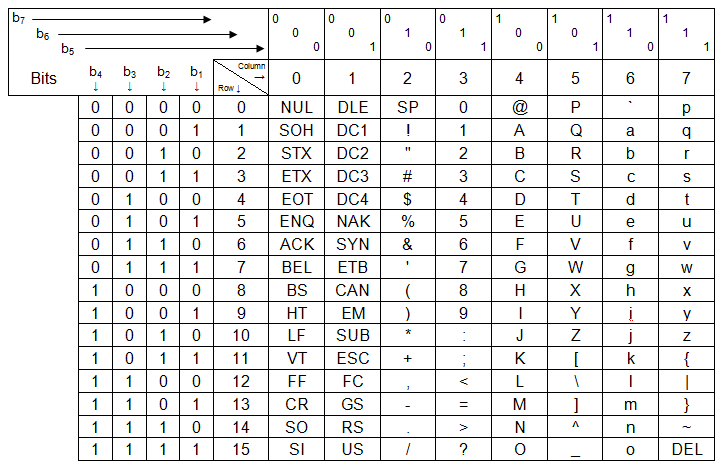
\includegraphics[scale=0.6]{./figures/ASCII.png}
  \caption{Encodage ASCII}
\end{figure}

\subsection{Code alphanumérique UTF-8}
Le code UTF-8 peut être vu comme une évolution majeure du code ASCII ; il vise à fournir un "répertoire universel de caractères codés", tout en conservant une retro-compatibilité avec
l'ASCII. Les symboles représentables en UTF8 englobent par exemple des caractères issus de langues étrangères (grec, hébreux, hiraganas japonais, etc), voire des musicaux (clé de sol, etc). L'UTF8 est, en 2017, utilisé par près de 90\% des sites web. Techniquement, un code UTF8 se présente comme une suite de 1 à 4 octets. Le nombre précis d'octets constitutifs
d'un code est lui-même encodé dans les bits de poids fort du code. Par exemple, lorsque le MSB vaut '0', cela signifie qu'un seul octet est nécessaire : cela correspond au code ASCII (il reste donc
7 bits pour coder les 128 caractères représentables en ASCII). Pour les codes au delà de l'ASCII, c'est le nombre de '1' en tête ("leading ones") du premier octet qui indique le nombre
d'octets qui suivront : par exemple un code UTF8 qui commence par "11110xxx" indique que le symbole codé nécessite 4 octets. Chaque octet suivant commence par "10".

\begin{center}
  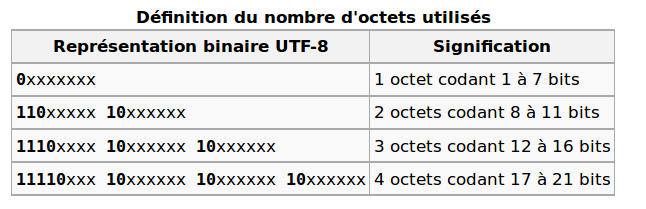
\includegraphics[scale=0.5]{./figures/utf8-w.png}
\end{center}

\begin{center}
  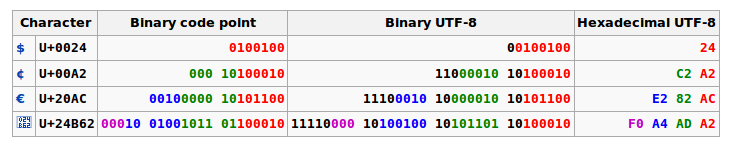
\includegraphics[scale=0.5]{./figures/utf8-example.png}
\end{center}
%===========================================================================================================
\section{Calcul en virgule fixe et en virgule flottante}

\subsection{Les nombres en virgule fixe}
Nous avons déja vu que les nombres qui possèdent une partie fractionnaire c'est-à-dire qui présentent une virgule après la partie
entière peuvent également se représenter en binaire ou dans tout autre base. On utilise simplement les puissances négatives de la
base en question.

$$ x = \sum_{i=-\infty}^{i=\infty} c_i.r^i, \mbox{avec } c_i \in \{0\dots (r-1)\} $$

En binaire, ces extensions s'appellent les ``décimales binaires'' : la première décimale binaire est $\frac{1}{2}$,
la seconde est $\frac{1}{4}$, la troisième est $\frac{1}{8}$ et ainsi de suite.\\

Dans certains processeurs de traitement du signal, on utilise une représentation des nombres dite {\it en virgule fixe} :
on restreint cette extension à une puissance donnée, afin que les opérations se fassent avec une position établie de la virgule
fixée, une bonne fois pour toute, ce qui simplifie l'architecture physique de l'unité de calcul. La position de la virgule est
alors connue et admise, au point où on peut l'oublier : cela revient à manipuler un simple entier. Par exemple, on peut associer
le nombre 125 à une mesure de 1.250 m. Pour une virgule placée au rang $k$, la différence entre deux nombres consécutifs
(appelée résolution) est égale $2^{-k}$ et sa dynamique (différence entre le nombre le plus grand et le plus petit) est réduite
à $2^{n-k}$, $n$ étant le nombre de bits du nombre.\\

Le calcul en virgule fixe est idéal dans le cas de l'addition : la place de la virgule n'est pas appelée à changer dans le
résultat. Ce n'est pas le cas de la mulitplication : pour deux nombres ayant 1 chiffre après la virgule, on obtient un résultat
qui possède 2 chiffres après la virgule. Il en est de même de 2 nombres de 2 chiffres chacun : le résultat est sur 4 chiffres,
ce qui peut provoquer des débordements. Enfin, deux nombres de 2 digits présentant une virgule à l'extrême gauche donneront un
résultat de multiplication à 4 chiffres après la virgule : il faudra tronquer le résultat...Bref : il est peut-être souhaitable
de conserver une liberté dans la gestion des virgules, quand cela est possible.

\subsection{Les nombres en virgule flottante. Norme IEEE 754}
Le calcul scientifique nous amène à des formules qui mélangent différents ordres de grandeur, peu compatibles avec
la représentation en virgule fixe. Les ordinateurs possèdent pour la plupart une unité en virgule flottante ; c'est
désormais le cas de 100\% des ordinateurs de bureau. Seuls certains processeurs embarqués n'en possèdent pas, car
l'unité de calcul flottante est consommatrice de surface. La représentation en virgule flottante est normalisée par
l'organisme IEEE, responsable de la standardisation de bon nombre de techniques, langages etc. Il s'agit ici de
s'assurer que les manipulations flottantes d'un programme ne dépendront pas de l'architecture de la machine : Intel,
AMD et. doivent fournir la même représentation. Il existe en réalité deux représentations normalisées IEEE 854 :
simple et double précision. On ne s'attarde ici que sur la première représentation.\\

\begin{center}
 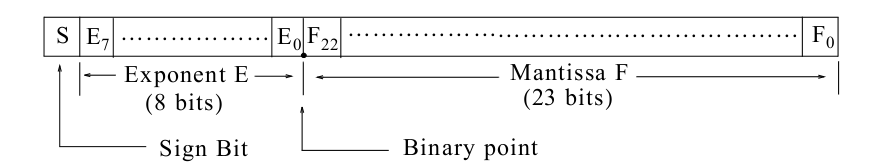
\includegraphics[scale=0.3]{./figures/ieee_854.png}
\end{center}

La représentation des flottants selon la norme IEEE simple précision se fait à l'aide de mots de 32 bits, ainsi constitués :
\begin{itemize}
\item un bit de signe, dénoté S : le $0$ représente le $+$ et le $1$ le $-$.
\item 8 bits d'exposant (7 à 0), dénoté $e$
\item 23 bits pour la partie fractionnaire, ou \textbf{mantisse} $f$, dénotés de 22 à 0. {\it e} et {\it f} sont toujours représentés en base 2, \underline{non complémentés à 2}.
\end{itemize}

La valeur absolue du nombre à représenter est normalisée selon la forme $1.f\times 2^e$. On notera que le premier '1' apparaissant dans cette forme n'est pas stocké, mais implicite.
Les 8 bits d'exposant présentent quelques particularités :
\begin{itemize}
  \item Les valeurs $00_{16}...FF_{16}$ représentent des codes spéciaux.
  \item Les valeurs $01_{16}...FE_{16}$ représentent des exposants courant de $2^{-126}$ à $2^{127}$.
  \item La valeur pôle est $7F_{16}=2^0=1$
\end{itemize}

\paragraph{Exemple}
Calculons la représentation du nombre $-3.25$ en IEEE 754-SP. On a : $-3.25=-11.01_2=-1.101 \times 2^1$
\begin{itemize}
  \item $s=1$
  \item $e=1+127=128=10000000_2$
  \item $f=10100000000000000000000$
\end{itemize}
D'où : $-3.25=11000000010100000000000000000000=c0500000_{16}$

\section{Manipulations numériques}

L'essentiel des techniques en logiciel embarqué consiste en des manipulations de {\it champs de bits} (bitfields), insérés au sein des nombres.
Un périphérique, par exemple, peut présenter au processeur plusieurs données dans un seul mot de 32 bits.

\subsection{Récupération d'un champ : masque hexadécimal}
Revenons à la représentation de la position (x,y).
Bien entendu, lorsque l'on utilise le nombre particulier Pos précédent,
il est nécessaire de connaître le mécanisme qui l'a créé, afin de récupérer
une coordonnée x ou y :
\begin{lstlisting}[
    label=listing:RubyTest,frame=single,
    float=h,
    caption=utilisation d'un masque hexadécimal en C,
    firstnumber=1,
    language=Ruby,
    basicstyle=\ttfamily,
    keywordstyle=\color{red},
    stringstyle=\color{blue}]
y = (0x0000FF) && Coord
\end{lstlisting}

Ce calcul permet d'extraire y du nombre Coord.
C'est un ET binaire, bit à bit, entre Coord et une constante exprimée en headecimal.
$0x0000FF$ a été créé de manière à annuler la contribution des bits de x dans Coord.
Pour cela les 4 digits hexadéciamaux sont effectivement à 0 ; ils représentent 16 bits
(4 fois 4 quartets) à 0. Quel que soit la valeur x, le ET bit à bit retournera des bits
à 0. A l'inverse, les 2 derniers quartets de la constante sont à $F$ et représentent
 donc 8 bits à 1. En conséquence, sur les 2 derniers quartets résultats, on retrouvera
 bien forcément la valeur de y, et elle seule, dans le résultat.



\subsection{Autres manipulations logicielles, au niveau bit}
La section précédente nous a permis de récupérer un champ particulier d'une donnée composée, grâce à une
 manipulation de bits. Il existe en fait de nombreuses manipulations qu'il est utile de connaître, notamment
 dans le domaine de la programmation pour des systèmes embarqués : les processeurs (et en particulier les micro-contrôleurs)
 actionnent et agissent sur leur environnement en écrivant et lisant des données précises stockées dans des circuits spéciaux appelés
 {\it registres}.

 A titre d'exemple, on propose un code écrit en langage C \footnote{Le langage C sera étudié en seconde année, pour les options STIC}
 qui réalise une boucle typique d'un système embarqué : la lecture d'une valeur détenue par un capteur (ici de simples boutons !),
suivie d'une action sur l'environnement, à savoir ici l'écriture des états des boutons sur des LEDs.

\begin{lstlisting}[language=C,frame=single]
#define Pushbuttons ((volatile long *) 0x10000050)
#define LEDS ((volatile long *) 0x10000010)
int main(void){
  long PBVal;
  while(1){
    PBVal = * Pushbuttons; // get the status of buttons : high or low
    *LEDS = PBVal; // display the status on LEDs
  }
}
\end{lstlisting}

 Pour les plus curieux  et à titre d'exemple, on donne ici une fonction (toujours écrite en langage C), qui permet d'initialiser (à 0) un registre particulier accessible par un micprocesseur.
 L'addresse du registre est ici $e0028008$. On indique au compilateur que ce registre n'est pas de son ressort à travers le mot clé "volatile" : le compilateur ne cherchera pas à réaliser
 d'optimisation sur ce registre. On accède au contenu par un {\it pointeur} (variable particulière qui contient l'addresse en question).

 \begin{lstlisting}[language=C,frame=single]
void clearReg(){
  (*((volatile unsigned int *) 0xe0028008))=0;
}
 \end{lstlisting}

 Ces registres sont à l'image de l'exemple de la position $(x,y)$, agglomérant plusieurs informations
 : par exemple, une alarme peut se manifester dans un bit de ce registre, à une position donnée (ex : le bit 7 du
 registre ``alarmes'' peut signifier ``porte non-verrouillée''). Il est donc important d'accéder à chacun des bits ou
 champs entiers de ces registres.

Le listing suivant propose quelques manipulations de champs de bits (applicables à à peu près tous les langages de programmations classiques).

\begin{lstlisting}[
    label=listing:RubyTest,frame=single,
    float=h,
    caption=Accès aux bits par programme informatique,
    firstnumber=1,
    language=C,
    basicstyle=\ttfamily,
    keywordstyle=\color{red},
    stringstyle=\color{blue}]
a = a | 0x4; /* mise a 1 du bit 2 de la variable a*/
a |=0x4; /* idem*/
b &= ~(0x4) /* mise a 0 du bit 2 */
b &= ~(1 << 2) /* idem, mais plus explicite*/
c ^= ~(1 << 5) /* inversion du bit 5*/
e >>=2 /* division de e par 4 */
\end{lstlisting}
% clear
% toggle
% divide



\subsection{Conversions et programmation}
Nous avons établi que $C_{2,3}(-2_{10})=6_{10}=110_2$. Comment trouver ces représentations,
à l'aide d'un langage de programmation s'exécutant sur votre ordinateur ? On peut écrire :

\begin{lstlisting}[
    label=listing:RubyTest,frame=single,
    float=h,
    caption=conversion signé vers non signé sur un nombre de bits restreint en langage Ruby,
    firstnumber=1,
    language=Ruby,
    basicstyle=\ttfamily,
    keywordstyle=\color{red},
    stringstyle=\color{blue}]
x = -2            % valeur a convertir
u = -2 & (2**3-1) % obtention de la valeur non signee. u=6
s = u.to_s(2)     % conversion en chaine de caracteres. s="110"
\end{lstlisting}

Pour comprendre cette manipulation, il faut savoir que les entiers signés sont codés sur 32 bits. Par conséquent, on peut établir
que la valeur $-2$ est représentée commme : $11\dots110_2$.

La seconde ligne consiste à masquer tous les bits au delà du troisième bit. Ces bits sont à 1, car ils représentent le bit
de signe.

\section{Vers la détection d'erreur entre émetteur et récepteur : bit de parité}
Lors de la transmission d'une donnée binaire codée sur plusieurs bits, il est fréquent que l'on lui adjoigne un bit supplémentaire, appelé {\it bit de parité}.
La valeur $0$ ou $1$ dépend des autres bits, de manière à ce que la somme totale des $1$ du code binaire soit paire. Ceci permet, à moindre frais, de s'assurer qu'une
erreur (simple) ne s'est pas produite lors de la transmission. En effet, le recepteur peut alors verifier la parité de la donnée reçue. L'hypothèse sous-jacente stipule
qu'une seule erreur binaire est tolérée. Au delà, il faudra rajouter des bits plus sophistiqués : code de Hamming, Turbo-codes etc.

\begin{figure}[htb!]
    \centering
    \begin{minipage}{0.45\textwidth}
        \centering
        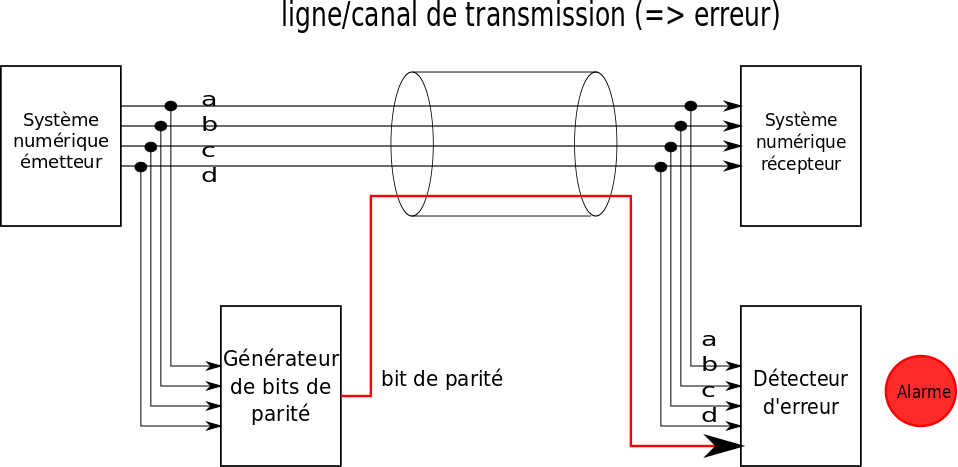
\includegraphics[width=1.1\textwidth]{./figures/parite-1.png} % first figure itself
        \caption{Emetteur, récepteur et canal bruité}
    \end{minipage}\hfill
    \begin{minipage}{0.45\textwidth}
        \centering
        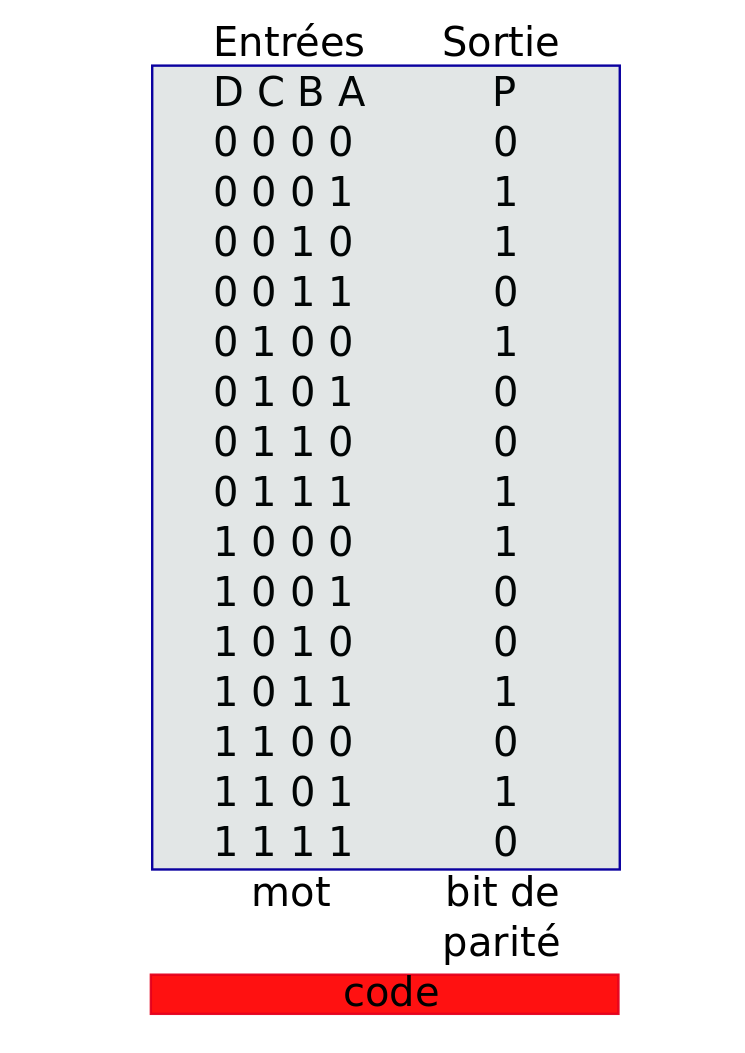
\includegraphics[width=0.4\textwidth]{./figures/parite-3.png} % second figure itself
        \caption{Table de vérité du bit de parité}
    \end{minipage}
\end{figure}


\section{Conclusion}
Ce chapitre vous a permi de rentrer de plain-pied dans les représentations numériques,
notamment avec la prise de connaissance de différents codes. Ce domaine est vaste ! Il existe d'autres codes
que nous n'avons pas aborder, comme les codes en excès de 3 où le code de Aïken.
Nous nous appuyerons sur ces premières connaissances afin de construire --bientôt-- nos
premières applications numériques.
Nous recommandons ici, en complément, la lecture de Bryant et O'Hallaron \cite{bryant} pour plus de détails sur la partie arithmétique.
Il est également intéressant de regarder d'autres présentations orientées sur la Théorie de l'Information comme Cover \& Thomas \cite{cover}.

\chapter{Logique booléenne}


\section{Introduction}

\begin{wrapfigure}[7]{r}{3.5cm}
  \vspace{-20mm}
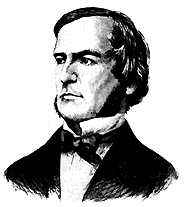
\includegraphics[width=4cm]{./figures/george_boole.jpg}
\end{wrapfigure}
Nous nous intéressons ici à une algèbre sur les propositions logiques : nous serons à même d'effectuer des calculs sur la logique à 2 valeurs : vrai ou faux.
C'est George Boole qui l'introduisit au milieu du \siecle{19}. Connu pour ses travaux sur les équations différentielles, il l'est encore plus lorsqu'il fait paraître
un traité qui fit date, intitulé {\it "An Investigation Into the Laws of Though"}, au titre très annonciateur. Son intention sous-jacente était de traduire des
idées et concepts en équations, puis d'effectuer des calculs sur la véracité de ces idées : là aussi, on peut rester admiratif devant tant d'intuition !
Pourtant, il semble que ses travaux sont longtemps restés cantonnés à des jeux de salons mondains.
A titre d'exemple, voici une énigme qui peut être résolue grace à l'algèbre de Boole :
on dispose de 3 boîtes A,B et C et de 3 jetons de couleur respective bleu, blanc et rouge. Chaque boîte possède un jeton. Sachant qu'une seule
proposition est vraie, déterminer le contenu de chaque boîte.

\begin{enumerate}
  \item la boîte A contient le jeton rouge.
  \item la boîte B ne contient pas le jeton rouge
  \item la boîte C ne contient pas le jeton bleu.
\end{enumerate}

Cette logique s'appelle également la {\it logique des propositions}. On pourra mettre en relation (on dit aussi "connecter") ces propositions grâce à l'algèbre de Boole.
C'est seulement au  \siecle{20} que Claude Shannon redécouvrit le pouvoir de modélisation de l'algèbre de Boole et son applicabilité
directe au domaine de l'Electronique.

\section{Définitions}


Soit $\mathbb{B}=\{0,1\}$ l'espace de Boole. Une variable booléenne simple est définie sur $\mathbb{B}.$
Il est également possible de travailler sur plusieurs variables : une variable booléenne {\bf générale} est un n-uplet $X=(x_1,x_2,\dots,x_n) \in \mathbb{B}$ et peut prendre $2^n$ valeurs. L
a valeur de $X$ est appelée un point. Un litéral est une variable booléenne simple ou son complément. Par exemple, $a$ et $\overline{a}$ sont deux littéraux distincts correspondant à la même
 variable.\\

Les opérations de l'algèbre de Boole sont les suivantes :
\begin{itemize}
\item La {\bf Conjonction} (ou produit logique) de deux variables (bits) : on parlera plus volontiers du {\bf ET} logique, dénoté par un signe croix ($\times$).
\item La {\bf Disjonction} (ou somme logique) de deux variables (bits) : on parlera plus volontiers du {\bf OU} logique, dénoté par un signe plus ($+$).
\item La {\bf Négation} (ou complémentation ou inversion) d'un seul bit : on parlera plus volontiers du {\bf NON}, dénoté par une barre au dessus de la variable ($\bar a$).
\end{itemize}

Ces opérations peuvent être représentées par des {\bf tables de vérité}, qui énumèrent explicitement les correspondances entre les entrées et les sorties :

\begin{center}
\begin{tabular}{|c c|c|}
  \hline
  $a$ & $b$  & $a \times b$ \\
  \hline
  0 & 0 & 0 \\
  0 & 1 & 0 \\
  1 & 0 & 0 \\
  1 & 1 & 1 \\
  \hline
\end{tabular}
\quad
\begin{tabular}{|c c|c|}
  \hline
  $a$ & $b$  & $a + b$ \\
  \hline
  0 & 0 & 0 \\
  0 & 1 & 1 \\
  1 & 0 & 1 \\
  1 & 1 & 1 \\
  \hline
\end{tabular}
\quad
\begin{tabular}{|c|c|}
  \hline
  $a$ & $\bar{x}$ \\
  \hline
  0 & 1 \\
  1 & 0 \\
  \hline
\end{tabular}
\end{center}

$x \times y$ vaut $1$ si $x$ vaut 1 {\bf et}  $x$ vaut 1, $0$ sinon.

$x + y$ vaut $1$ si $x$ vaut 1 {\bf ou}  $x$ vaut 1, $0$ sinon.

$\bar{x}$ vaut $1$ si $x$ vaut 0, $0$ sinon.

Il est à noter que le OU logique n'a pas la même signification ici et dans le langage de la rue : lorsqu'on utilise le OU dans la vie de tous les jours, il s'agit d'une exclusion (c'est l'un
e ou l'autre des variables qui est sensée être vraie). On parlera alors de OU {\it exclusif}, alors que le OU ($+$) est un OU {\it inclusif}. Retenez toutefois que le OU {\it exclusif} est é
galement utilisable et utilisé en électronique. Son symbole est généralement le $\oplus$.

\subsection{Axiomes de l'Algèbre de Boole}
Soit {\it x,y,z} des variables booléennes. Les axiomes de l'Algèbre de Boole sont les suivants :

\begin{enumerate}
%% \item Alors $x = 0$ ou $x = 1$ . Si $x=0$, alors $\bar{x} = 1$ , et vice versa.
%% \item $0 \times 0 = 0$
%% \item $0 \times 1 = 1 \times 0 = 0$
%% \item $1 \times 1 = 1$
%% \item $0 + 0 = 0$
%% \item $0 + 1 = 1 + 0 = 1$
%% \item $1 + 1 = 1$
\item  {\bf $+$ est associatif} :  $x+(y+z)=(x+y)+z$
\item  {\bf $\times$ est associatif} :  $x\times(y\times z)=(x\times y)\times z$
\item  {\bf $+$ est commutatif} :  $x+y=y+x$
\item  {\bf $\times$ est commutatif} :  $x\times y=y\times x$
\item  {\bf existence d'un élément neutre pour $+$} :  $\exists 0 / x+ 0 = x$
\item  {\bf existence d'un élément neutre pour $\times $} :  $\exists 1 / x \times 1 = x$
\item  {\bf $\times$ est distributif sur $+$} : $x.(y+z)=x.y+x.z$
\item  {\bf $+$ est distributif sur $\times$} : $x+(y.z)=(x+y).(x+z)$. Ce résultat est plus surprenant !
\item  {\bf existence du complément}
\end{enumerate}

\subsection{Principaux théorèmes de l'Algèbre de Boole}

\begin{enumerate}
\item {\bf $+$ est idempotent} : $x+x=x$
\item {\bf $\times$ est idempotent} : $x \times x=x$
\item {\bf $1$ est absorbant pour $+$} : $x+1=1$
\item {\bf $0$ est absorbant pour $\times$} : $x\times 0=0$
\item {\bf unicité du complément}
\item {\bf complément du complément} : $\overline{ ( \overline{x} ) }=x$
\item $x+x.y = x$
\item $x \times (x + y) = x$
\item $x + \bar{x} \times y = x +y$
\end{enumerate}

\subsection{Théorèmes de De Morgan}

Parmi les théorèmes de l'algèbre de Boole, les théorèmes de de Morgan sont particulièrement intéressants et utiles pour la suite.
Observons le tableau suivant, qui expose le calcul de deux fonctions $f_1(a,b)=\overline{a+b}$ et $f_2(a,b)=\overline{a}.\overline{b}$.

\begin{center}
   \begin{tabular}{|c|c|c|c|c|c|c| }
     \hline
     a & b & $a+b$ & $f_1=\overline{a+b}$ & $\overline{a}$ & $\overline{b}$ & $f_2=\overline{a}.\overline{b}$ \\ \hline \hline
     0 & 0 &     0 &                   1  &              1 &              1 &                              1  \\ \hline
     0 & 1 &     1 &                   0  &              1 &              0 &                              0  \\ \hline
     1 & 0 &     1 &                   0  &              0 &              1 &                              0  \\ \hline
     1 & 1 &     1 &                   0  &              0 &              0 &                              0  \\ \hline
   \end{tabular}
 \end{center}

Ce calcul démontre que les deux fonctions sont en fait égales :
$$\boxed{\overline{a+b}=\overline{a}.\overline{b}}$$
On peut également démontrer que :
$$\boxed{\overline{a.b}=\overline{a}+\overline{b}}$$

Ce résultat peut bien entendu se généraliser pour plus de 2 variables. La manière de retenir se résultat consiste à s'apercevoir que
"la descente de la barre sur les opérandes" s'accompagne du changement de l'opération "+" en "*" (et vice versa)

\section{Représentation des fonctions booléennes}

\subsection{Monôme}
Un monôme $m$ est un produit de $p$ variables simples distinctes sous formes normales ($x$) ou complémentées ($\overline{x}$). Un monôme canonique est un monôme de degré $n$ dans $\mathbb{B}
^n$.

\subsection{Fonctions booléennes}
Une fonction booléenne est une fonction de $\mathbb{B}^n$ vers $\mathbb{B}^m$.

\begin{itemize}
\item $n=1,m=1$ : la fonction est dite fonction simple d'une variable simple.
\item $n>1,m=1$ : la fonction est dite fonction simple d'une variable générale.
\item $n>1,m>1$ : la fonction est dite fonction générale d'une variable générale.
\item $n=1,m>1$ : la fonction est dite fonction générale d'une variable simple.
\end{itemize}

{\bf Exemple} : la fonction $F(a,b)=a+b$ est une fonction booléenne simple d'une variable générale $(a,b)$

\subsection{Fonction booléenne incomplète ou $\phi$-booléenne}

Si $F$ n'est pas définie en $X\in \mathbb{B}^n$, on a l'habitude de poser $F(X)=\phi$, où $\phi$ représente à la fois $0$ et $1$ superposés. $\phi$ représente la valeur indéfinie (en anglais
 ``don't care''), qui signifie que la fonction peut prendre indistinctement la valeur $0$ ou $1$ en ce point. On dit que $F$ couvre un point $X$ si $F(X)=1$.

\subsection{Minterm et maxterms}
Nous avons établi qu'une variable booléenne peut apparaître sous sa forme normale ou complémentée.
Par ailleurs, le produit de deux variables $A$ et $B$ conduit à $2^2=4$ combinaisons possibles : $A.B,\overline{A}.B,A.\overline{B}$ et $\overline{A}.\overline{B}$. Ces $4$ s'illustrent sur
un diagramme de Venn. Ces $4$ produits sont des {\it minterms} ou {\it produits standards}. En d'autres mots, un minterm est un produit composé de deux variables (ou plus) ou de leur complém
ents.

\subsection{Décomposition de Shannon et Arbres de décision binaires}
La décomposition de Shannon ne sera pas utilisée dans ce cours, mais mérite toutefois d'être évoquée. En effet, elle est à la base des représentations manipulables par les ordinateurs : il f
aut se projeter dans des systèmes numériques composés de millions d'équations logiques, pour lesquels il est important de manipuler efficacement ces notions ! Cette décomposition s'écrit de
la manière suivante :

$$F(x_1,x_2,\dots,x_n)=x_1.F(1,x_2,\dots,x_n) + \overline{x_1}.F(0,x_2,\dots,x_n)$$

%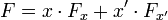
\includegraphics[scale=0.5]{../figures/shannon_0.png}
%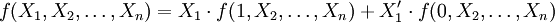
\includegraphics[scale=0.5]{../figures/shannon.png}

Son intérêt est qu'il est possible de l'appliquer récursivement. Cette décomposition s'illustre de la manière suivante , appelée diagrammes (ou arbres) de décisions binaires (BDD : binary de
cision diagrams) :

%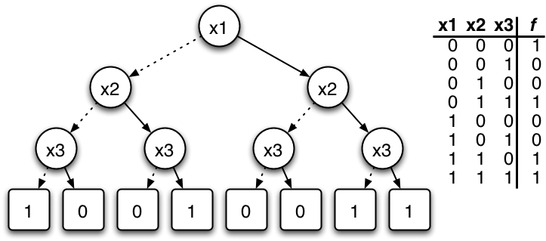
\includegraphics[scale=0.3]{../figures/bdd.jpg}

Cette décomposition a permi l'essor d'outils de preuves formelles sur les circuits --mais pas seulement-- : les ``solvers'' de satisfiabilité par exemple permettent de trouver s'il existe un
e variable totale qui rende une formule booléenne vraie (problème SAT). C'est un problème très difficile \footnote{SAT est le premier problème connu dit NP-complet...} !

En réalité, le terme de BDD est généralement associé à ROBDD : Reduced Ordered Binary Decision Diagram. L'intérêt des ROBDD est qu'il présente une forme canonique (unique) pour une fonction
donnée et quel que soit l'ordre d'évaluation des variables. Cette propriété le rend très utilse dans la recheche d'équivalence entre 2 circuits : implémentent-ils intrinsèquement la même for
mule, bien qu'ils se présentent sous une forme électronique différente ?

%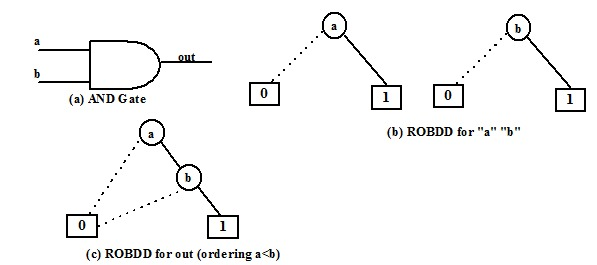
\includegraphics[scale=0.3]{../figures/robdd_and.jpg}
%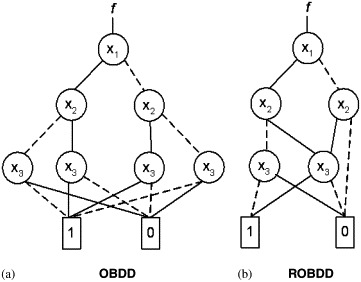
\includegraphics[scale=0.3]{../figures/obdd.jpg}
%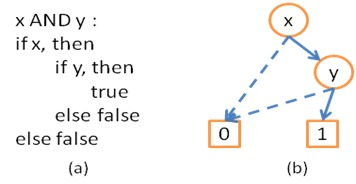
\includegraphics[scale=0.3]{../figures/bdd-prog.jpg}

\section{Simplification des fonctions booléennes}

\subsection{Par calcul algébrique}

La simplification d'expressions booléennes est un exercice difficile --y compris pour les ordinateurs qui les effectuent--, mais qui est nécessaire pour
optimiser le matériel. L'exemple suivant montre un exemple minuscule. Les deux signaux de sortie sont totalement identiques du point de vue logique : en fait
, on n'avait besoin d'aucune porte logique !

\begin{center}
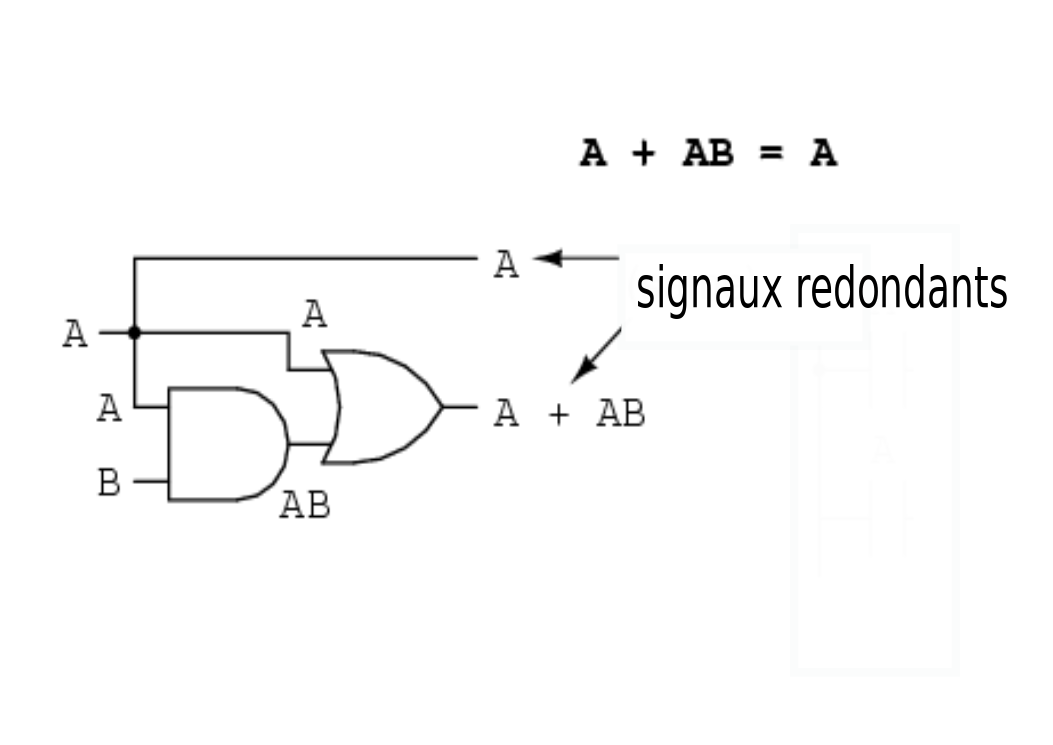
\includegraphics[scale=0.2]{./figures/redondance.png}
\end{center}

Cet exemple suggère également comment simplifier le circuit, par application des règles de composition algébrique vues précédemment. Voici le cheminement que l'on peut utiliser :
\begin{enumerate}
\item $A+A\times B$. Factorisons par $A$
\item $A(1+B)$. Appliquons l'identité $1+B=1$
\item $A\times 1$. Il s'en suit :
\item $A$
\end{enumerate}

Toutefois, la bonne application successive de ces règles est difficile pour des formules complexes. Cette application dépend de votre capacité à ``sentir'' la simplification...Il existe heur
eusement une autre méthode, plus mécanique.

\subsection{Par tableau de Karnaugh}
Les tableaux de Karnaugh permettent d'appliquer de manière mécanique des simplifications qui marchent à coup sûr. Ces tableaux sont en fait un ensemble de cases.
En général, une expression booléenne à $n$ variables peut être représentées par un tableau de Karnaugh à $2n$ cases, où chaque case représente une ligne d'une
table de vérité équivalente. Dans la méthode des tableaux de Karnaugh, il est nécessaire de disposer les entrées du tableaux d'une manière particulière : sans
cette disposition spéciale, la méthode ne peut s'appliquer. Cette manière particulière consiste à s'arranger afin que des cases contigues ne diffèrent que
d'une seule variable. On retrouve ici le code de Gray. Lorsque les entrées sont correctement énumérées, on peut disposer les monômes de la fonction à simplifier
dans ce tableau. Il est recommandé d'écrire au préalable la fonction logique sous la forme de sa table de vérité : il ne faudra pas confondre cette table de vérité initiale
et le tableau de Karnaugh associé ! Placer les monomes dans le tableau consiste à détecter les '1' de la fonction, dans sa table de vérité, et disposer ces '1' dans le tableau
de Karnaugh. Dès lors de ces monômes sont correctement reportés dans le tableau, on cherche des regroupements de '1' : on cherche précisément les regroupements
de '1' qui présentent un nombre d'éléments qui soit une puissance de 2 : 2, 4, 8 , 16 etc...  Ces regroupements doivent être soigneusement entourés. Du fait de l'adjacence des entrées du tableau, ces regroupements induisent
une simplification. Plus le nombre d'éléments regroupés est élevé, plus les simplifications seront importantes. Si aucun regroupement n'est possible, cela signifie qu'aucune simplification
ne peut s'appliquer.\\

Avant de nous lancer, prenons soin de remarquer que l'adjacence des cases fonctionne également sur les bords des tableaux : le haut et le bas sont adjacents ! Ainsi que la gauche et la droite ! Mieux encore,
les 4 angles sont également adjacents. Cela signifie qu'un ensemble de quatre '1' disposés aux quatre angles se prêtent à une simplifications booléenne.\\

Observons un premier cas : simplifions la fonction $f_1(a,b,c)=a.b.\overline{c}+a.b.c$. La simplifications algébrique est ici triviale, mais passons par un tableau de Karnaugh.
Les deux monômes, disposés dans le tableau, permettent un regroupement de 2 cases. La variable 'c' est ici simplifiable, {\it du fait de cette adjacence} (le retour à la méthode algébrique le confirme). La fonction
vaut donc au final $f_1(a,b,c)=a.b$.\\

\begin{center}
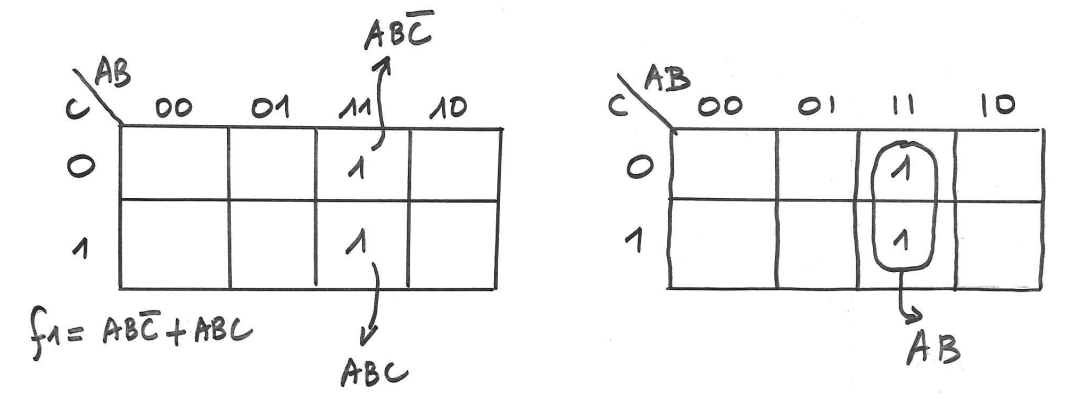
\includegraphics[scale=0.2]{./figures/karnaugh_00.png}
\end{center}

On peut s'autoriser désormais à utiliser cette méthode pour des simplifications moins triviales.
Ainsi, la fonction $f(a,b,c,d)=a.b+\overline{a}.b.\overline{c}.d+\overline{a}.b.c.d + a.\overline{b}.\overline{c}.\overline{d}$ vaut,
simplifiée $f(a,b,c,d)=a.b+b.d+a.\overline{c}.\overline{d}$
\begin{center}
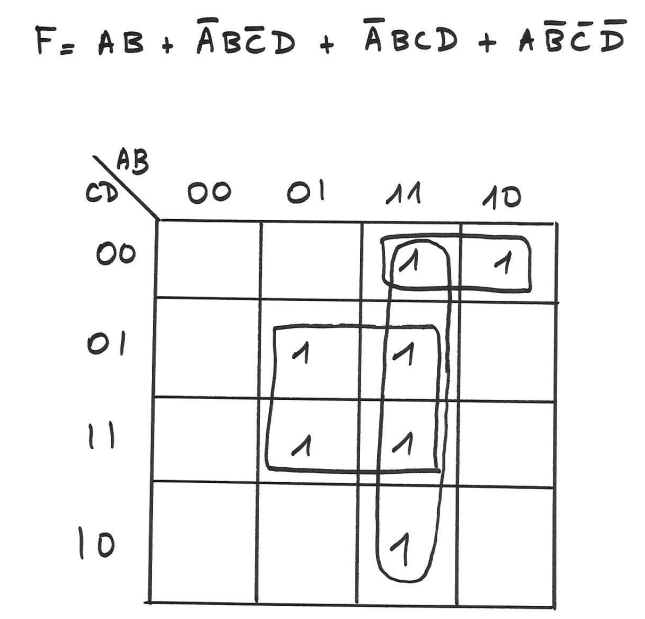
\includegraphics[scale=0.2]{./figures/karnaugh_01.png}
\end{center}


%% \subsection{Autres méthodes}
La bonne nouvelle est que ces simplifications ont été automatisées dans des logiciels.
Au cours de l'Histoire, plusieurs méthodes ont vu le jour : notamment l'algorithme de Quine Mac Cluskey, puis des méthodes symboliques, à base de BDD, encore plus puissantes.
Toutefois, les algorithmes soulèvent des problèmes de
complexité informatique insoupçonnés : il n'existe pas de méthodes qui puisse garantir le caractère optimal du résultat, pour tous les cas !

\section{Conclusion}
Ce chapitre nous a permis de nous familiariser avec l'algèbre de Boole. Il s'agit là de bases essentielles
à la mise en équation de problèmes d'électronique numérique. Ce socle solide va nous permettre d'aborder l'ensemble de la conception en Electronique
et Informatique (embarquée ou non) de manière sereine. Dans le chapitre suivant, nous allons directement chercher à représenter ces équations issues
de l'algèbre de Boole par de véritables circuits électroniques.

\chapter{Circuits combinatoires}
\minitoc
\section{Définition}
Un système numérique est dit combinatoire si toutes ses sorties, à tout instant $t$, ne dépendent que de la combinaison de
ses valeurs d'entrées et aucunement des sorties précédemment calculées. Les {\it systèmes combinatoires n'ont pas de mémoire d'un état interne passé}, alors que c'est le cas pour les systèmes séquentiels, caractérisé par cet état.
Notons que, dans le détail de la physique sous-jacente, les choses sont un peu plus compliquées :
on peut en effet noter que, même dans un circuit combinatoire, il existe un effet mémoire lié aux différentes mini-capacités
(condensateurs) qui sont susceptibles d'emmagaziner de l'énergie (sur les connexions etc). Ainsi les sorties dépendent des valeurs des entrées à un instant $t-\delta$
Toutefois, on sait que si l'on attend suffisamment longtemps, cet effet mémoire s'évanouit...\\

Il faut donc retenir l'intuition des systèmes combinatoires :
après avoir positionné des entrées, et lorsqu'on attend un temps suffisant (le $\delta$ de la définition),
on verra un résultat en sortie, qui ne dépend que des entrées (supposées stables)...

\section{Portes logiques de base}

Le tableau suivant résume les principales portes logiques dont nous ferons usage. Ces portes se présentent sous plusieurs formes équivalentes :
graphiques, équationnelles ou tabulées. Il faudra être à même de basculer d'une de ces représentations à une autre. Dans le tableau figurent deux types de
symboles : à gauche on trouve les symboles IEC, et à droite les symboles ANSI (dits "américains"). Les symboles IEC ne sont quasiment pas utilisés désormais, et
nous conseillons ici vivement de leur préférer les symboles américains. L'IEC reste utilisé dans le domaine du contrôle industriel, qui n'est qu'une infime partie de
l'Electronique traitée ici, dans sa généralité.

\begin{center}
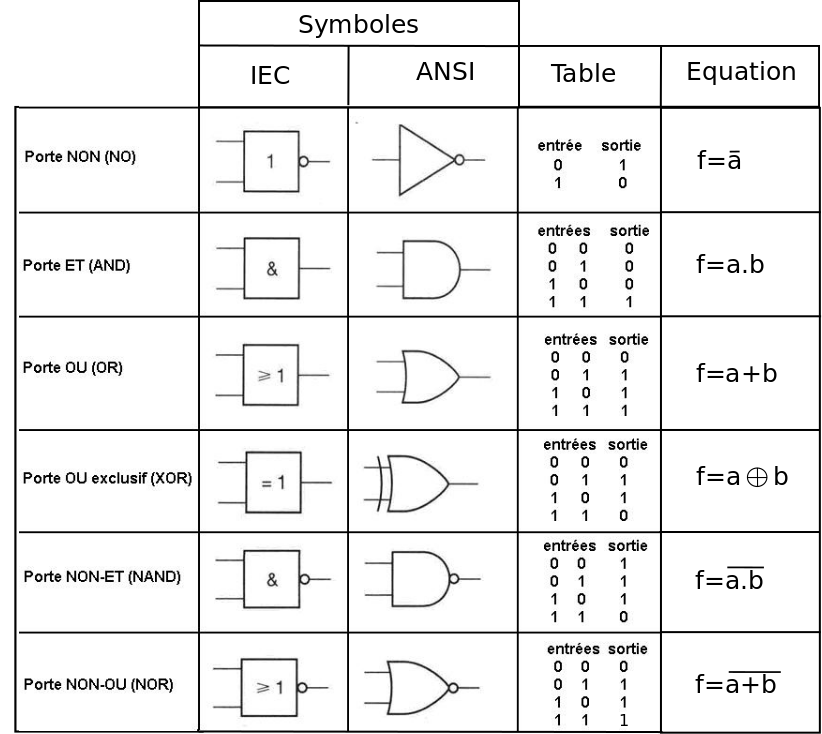
\includegraphics[scale=0.4]{./figures/table_verite.png}
\end{center}

\paragraph{Première approche : et, ou, non}
Les portes logiques de base reflètent directement les opérations élémentaires de l'algèbre de Boole : conjunction, disjonction et
négation. Ces portes permettent de construire directement un circuit électronique à partir d'une (ou plusieurs) expression(s) booléenne(s) donnée(s). L'assemblage
telles portes logiques (auquelles on ajoutera bientôt un élement séquentiel) forme une {\it netlist} (ou, en français, {\it liste d'interconnexions})
. Dans des cas réels, cette netlist peut contenir plusieurs millions de tels élements de base. A l'inverse, à partir d'un schéma de
netlist, il est possible de revenir à une ou plusieurs équations booléennes. Tout système numérique peut être envisagé comme tel : un vaste ensemble (graphe) de portes logiques.

\paragraph{Deuxième approche : autres portes logiques}
Dans la pratique, il est utile de pouvoir également disposer de portes logiques comme le XOR (ou exclusif), Nand, Nor à deux  entrées, mais également à plusieurs entrées (AND3, AND6 etc).
Technologiquement, ces portes complexes sont construites {\it à façon} par un {\it fondeur}. Parmi ces fondeurs, on trouve des sociétés comme STMicroelectronics, Samsung, Texas Instrument, IBM, TSMC, Intel etc.
Certaines d'entre elles ne produise de circuits que pour leur propre fabrication (Intel) tandis que d'autres (TSMC) permettent à une société tierce d'accéder à ces fonderies.

\paragraph{Troisième approche : non-et (nand)}

Une seconde manière de parler des portes logiques de base est de se pencher sur les propriétés de l'algèbre de Boole. On peut se rendre à l'évidence que les trois fonctions AND, OR et NOT
peuvent se calculer à l'aide d'une autre porte logique {\it unique}, qui devient ainsi la brique élémentaire de tout circuit numérique. Il s'agit de la porte NAND (non-et). Le calcul est également
possible avec le NOR, mais il est de tradition de considérer uniquement le NAND. Pour simplifier l'écriture, posons $\overline{a.b}=a \odot b$. On a donc $a \odot 1=not(a)$.
Prenons la formule $y=a+b$ et exprimons là à l'aide de $\odot$. Posons $\alpha=a$ et $\beta=b$.  On a donc :

\begin{align}
y &=  a + b \\
y  &= \overline{\alpha.\beta}\\
y  &= \alpha \odot \beta\\
y &= (a \odot 1) \odot (b \odot 1)
\end{align}

De même, on peut démontrer que :
\begin{align}
y &=  a.b \\
y  &= \overline{\alpha}.\overline{\beta}\\
\end{align}
d'où :
\begin{align}
\overline{y}  &=  \overline{\overline{\alpha}.\overline{\beta}}\\
  &=  a \odot b
\end{align}
et : $$y=(a \odot b) \odot 1$$

Il est donc possible d'exprimer toute la logique booléenne à l'aide du NAND, et ainsi construire n'importe quel circuit à l'aide de la porte logique NAND \footnote{Un livre d'introduction aux circuits profite de cette curiosité et s'intitule "Nand to Tertis"}.
Au dela de cette curiosité mathématique, il se trouve qu'en terme de transistors, il est plus facile de réaliser les portes NAND et NOR que des portes non complémentées.

\section{Fonctions logiques "complexes"}

\paragraph{Assemblage de portes logiques}

En s'en tenant au 3 portes logiques précédentes, on peut connecter les sorties des unes aux entrées des autres de manière à réaliser des fonctions de plus plus complexes, à l'image
de la fonction présentée en début de ce chapitre. Cet assemblage ne nécessite pas de précautions particulières, alors cela était nécessaire en électronique analogique (adapation d'impédance etc).
Il faudra toutefois veiller à ne pas "chaîner" un "trop" (cela reste à définir...) grand nombre de portes logiques les unes derrière les autres : bien que fonctionnellement correct, un tel assemblage
a tout lieu d'affecter la performance finale du circuit : nous allons en parler dans un paragraphe à suivre.

\paragraph{Notion de "Nuage combinatoire"}
Cet assemblage de portes logiques représente une fonction mathématique qui associe, à plusieurs entrées logiques, plusieurs sorties logiques. Nous allons rapidement
créer des fonctions logiques de plus en plus complexes : une fois qu'elles seront établies, {\it une bonne fois pour toutes}, il n'y aura plus lieu d'en étudier la structure.
Très rapidement, nous chercherons donc à {\it abstraire ces fonctions} : les langages de description matériel commme VHDL nous y aideront notamment, car de simples constructions
du langage permettront, en réalité, de "parler" de ces fonctions. Ainsi la simple addition numérique, constituée d'un grand nombre de porte logiques, sera simplement abstraite par le symbole "+", ce qui
est fort pratique ! De même, au lieu de décrire des multiplexeurs, on sera bientôt tenté de les substituer par un "if..then else" du langage. Mais sans en référer à VHDL, il est
parfois pratique de réaliser {\it graphiquement} ces fonctions : il n'est donc pas rare de remplacer la fonction numérique par un simple "nuage". Il s'agit d'un nuage "combinatoire".
L'assemblage d'"ordre supérieur" de tels nuages nous permettra de passer une autre échelle et concevoir des circuits encore plus complexes, en appliquant des "patterns" ou "motifs de conception".

\section{Mapping technologique sur circuits discrets}
Pendant longtemps, les ingénieurs disposaient de circuits {\it discrets}, se présentant sous la forme d'un boitier bien caractéristique, avec un nombre
de "pattes" (entrées et sorties) très limité (une dizaine). Pour concevoir un système, il s'agissait de sélectionner les bons boîtiers et de réaliser les soudures
apropriées pour effectuer la transition entre la netlist "théorique" et ces composants discrets. C'était un travail d'ingénieur des années 1970 et 80 !
A l'heure actuelle (2017) et depuis déjà bien longtemps, cette sélection se fait désormais par des algorithmes, au sein de programmes complexes (synthétiseurs logiques). Le nombre d'équations logiques, lui-même,
dépasse par ailleurs les capacités d'un être humain à les gérer. Surtout, ces composants discrets ont quasiment disparu, au profit de composants programmables (FPGA),
sur lesquels nous reviendront. Précisons que, sur ces composants programmables, le mapping
technologique garde tout son sens, puisqu'il s'agit encore de "mapper" une netlist théorique sur un ensemble de composants.

\begin{figure}[htb!]
  \centering
  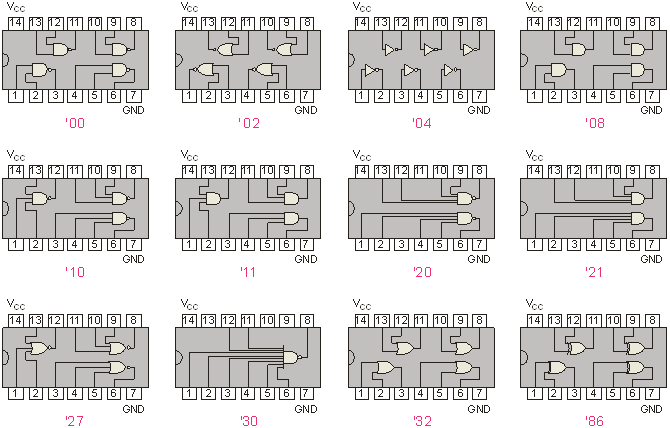
\includegraphics[width=10cm]{./figures/paste_image31.png}
  \caption{Exemple de circuits de la (mythique !) série 74, des années 70 et 80.}
\end{figure}


\section{Chemin critique et fréquence de fonctionnement}
La notion de chemin critique est d'une importance capitale. Il permet de calculer la fréquence maximale à laquelle on pourra soumettre un nouveau jeu d'entrées au circuit, sans perturber le calcul précédent. Cette fréquence
détermine {\it in fine} les performances finales de votre ordinateur.\\

Souvenons nous que, physiquement, nous avons affaire une interconnexion de composants, qui possèdent leurs propres resistance et capacité (et une inductance non significative). Un simple transistor possède un tel modèle équivalent...
Un signal électrique se présentant sur une entrée mettra un certain temps à agir sur les sorties du circuit : ce délai est directement relié à la capacité. Si on considère non plus une seule entrée, mais un ensemble d'entrées, la question que l'on peut se poser est la suivante : comment déterminer, parmi ces signaux, celui qui mettra le plus de temps
à se propager vers les sorties ? Pour cela, il suffit de parcourir la netlist et détecter {\it le plus long chemin entre les entrées et les sorties}.

Ce chemin est précisément le chemin combinatoire critique.
On fait généralement un abus de langage (toléré !) en associant ce chemin critique avec le {\it temps de propagation calculé sur ce chemin} : il faut connaître le temps caractéristique de traversée de chaque porte, ainsi que le temps de propagation sur chacun des fils qui les relient. En pratique,
des algorithmes calculent ce temps. Dès lors que l'on connait ce temps, on sait que c'est le laps de temps minimum pendant lequel, le circuit, {\it dans son intégralité}, ne pourra être utilisé pour un nouveau calcul. Si l'on possédait
un oscilloscope suffisamment précis, on pourrait constater, au cours de ce calcul, qu'une très grande agitation règne sur chacun des fils, et que cette agitation semble se propager des entrées vers les sorties, de manière anarchique.
Lorsque cette "vague" est passée, les fils de sortie se sont enfin stabilisés : on peut lire la sortie combinatoire. A l'inverse, si au cours de ce temps, on s'ingénie à vouloir utiliser la sortie, elle sera immanquablement fausse et instable.\\

Pour calculer la fréquence finale, on peut, {\it en première approximation} prendre l'inverse de ce temps \footnote{Nous verrons plus loin qu'il faut lui adjoindre deux autres composantes temporelles, liées aux bascules D}.
$$F_{max} \approx \frac{1}{t_{critic}}$$

\begin{center}
  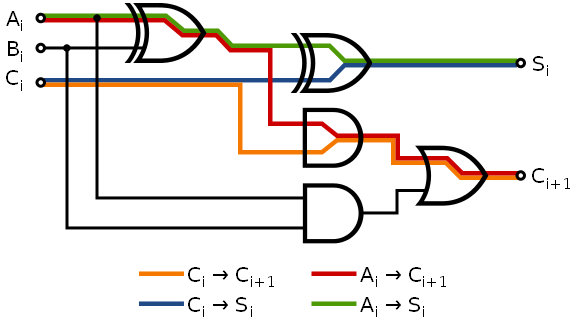
\includegraphics[width=6cm]{./figures/chemin-critique.png}
\end{center}

Cette "vague" fort complexe ne semble guère propice à l'élaboration de systèmes un tant soit peu élaborés...
Fort heureusement, nous serons rapidement en mesure de nous permettre d'"oublier" totalement ces phénomènes microscopiques, pour nous
concentrer sur l'essence des services macroscopiques que devra déliver notre système. Cette "libération" passe par la notion de circuits séquentiels.

\section{Arithmétique de base}
Nous abordons ici l'utilisation de portes logiques combinatoire afin d'élaborer des opérateurs de calculs "classiques" : additions d'entiers, multiplications etc.
On suppose d'emblée que l'on dispose d'{\it entrées} et de {\it sorties} numériques : il s'agit d'un ensemble de fils présentant (chacun) une tension 0 ou 5 Volts (selon la technologie, ces tensions peuvent varier).
Pour véhiculer deux opérandes A et B, il faut connaître la dynamique des valeurs que l'on veut traiter pour A et B : à partir de cette dynamique, on dispose d'un ensemble de fils
pour A et d'un ensemble de fils pour B, etc.

\subsection{Additionneur}
Il existe un grand nombre de manière d'assembler les portes logiques pour réaliser un calcul comme un additionneur.
La plus traditionnelle consiste à d'abord étudier le {\it demi-additionneur} (1 bit),
puis l' additionneur 1 bit {\it complet} (qui s'appuiera sur le demi-additionneur), puis chercher à étendre cet addition à des opérandes à plusieurs bits. Au coeur du procédé, on procède en utilisant le même algorithme
que celui enseigné dans notre enfance : on effectue une addition sur les digits les plus à droite, et on continue vers la gauche, en "marquant" d'éventuelles retenues.

\paragraph{Demi-additionneur 1 bit}
On parle de demi-additionneur afin de signifier qu'on ne s'intéresse pas, dans un premier temps, à la retenue entrante.
Le table de vérité et le circuits logique correspondant sont représentés ici. Les variables $s$ et $c$ dénotent la somme et la retenue (sortante).
Ce circuit s'appelle donc un demi-additionneur et est représenté par le symbole "HA" (half adder)
\begin{center}
   \begin{minipage}[t]{4cm}
     \vspace{0pt}
     \centering
     \begin{tabular}{|c|c||c|c|}
       \hline
       a & b & s & c \\ \hline
       0 & 0 & 0 & 0    \\ \hline
       0 & 1 & 1 & 0    \\ \hline
       1 & 0 & 1 & 0    \\ \hline
       1 & 1 & 0 & 1    \\ \hline
     \end{tabular}
   \end{minipage}%
   \begin{minipage}[t]{5cm}
     \vspace{0pt}
     \centering
     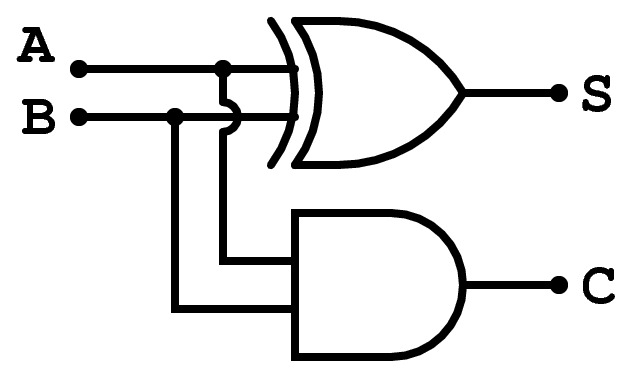
\includegraphics[width=3cm]{./figures/half_adder.jpg}
   \end{minipage}
   \begin{minipage}[t]{5cm}
     \vspace{0pt}
     \centering
     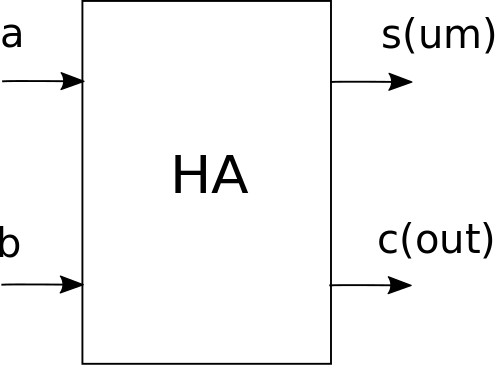
\includegraphics[width=3cm]{./figures/ha.png}
   \end{minipage}

\end{center} % added ending }



\paragraph{Additionneur 1 bit}

On introduit désormais la retenue entrante, afin de réaliser une addition sur n'importe quelle "colonne" de digits.
Un calcul permet de nous rendre compte que le demi-additionneur précédent peut être réutilisé. Il s'agit ici de notre premier
{\it assemblage hierarchique} de circuits.

\begin{center}
   \begin{minipage}[t]{4cm}
     \vspace{0pt}
     \centering
     \begin{tabular}{|c|c||c|c|c|}
       \hline
       a & b & $c_{in}$ & S & $C_{out}$ \\ \hline
       0 & 0 &   0 & 0 &         0 \\ \hline
       0 & 0 &   1 & 1 &         0  \\ \hline
       0 & 1 &   0 & 1 &         0  \\ \hline
       0 & 1 &   1 & 0 &         1  \\ \hline
       1 & 0 &   0 & 1 &         0 \\ \hline
       1 & 0 &   1 & 0 &         1  \\ \hline
       1 & 1 &   0 & 0 &         1  \\ \hline
       1 & 1 &   1 & 1 &         1  \\ \hline

     \end{tabular}
   \end{minipage}%
   \begin{minipage}[t]{5cm}
     \vspace{-5pt}
     \centering
     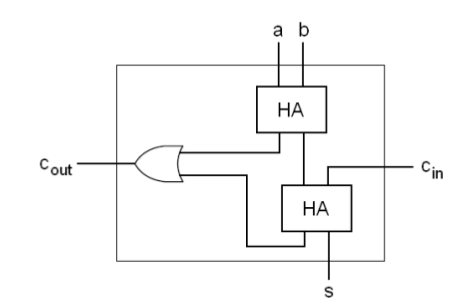
\includegraphics[width=5cm]{./figures/add-5.png}
   \end{minipage}
   \begin{minipage}[t]{5cm}
     \vspace{0pt}
     \centering
     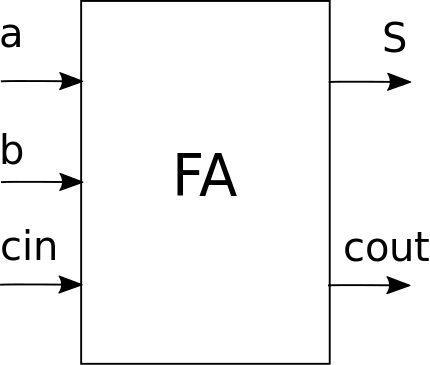
\includegraphics[width=3cm]{./figures/full_adder.png}
   \end{minipage}
\end{center} % added ending }

Le calcul évoqué est exposé ici. Au préalable on établit l'égalité suivante où $\oplus$ représente le {\it ou exclusif}:
$$\barre{a\oplus b}=\barre{a.\barre{b}+\barre{a}.b}=(\barre{a}+b).(a+\barre{b})=\barre{a}.\barre{b}+a.b$$
On a désormais :
\begin{align}
S  &= a.\barre{b}.c_i + a.b.c_i + a.\barre{b}.c_i + a.b.c\\
   &= a.(a\oplus c_i) + a (b\oplus c_i)\\
   &= a \oplus b \oplus c_i
\end{align}
De même, on trouve : $c_o=a.b+(a\oplus b).c_i$.
Le demi additionneur peut donc effectivement être ré-utilisé judicieusement, comme dessiné sur la figure précédente.

\paragraph{Additionneur {\it n} bits}
La manière la plus naturelle (mais pas la plus efficace !) consiste à chaîner les retenues sortantes et entrante : on parle d'{\it additionneur à propagation de retenue} ou {\it Ripple-carry Adder}.
Nous présentons ici un additionneur 4 bits avec retenue entrante. En général cette retenue est fixée à 0, mais nous verrons un peu plus loin qu'elle peut également être très utile. En exercice, on peut tenter de déterminer le chemin critique de ce circuit (l'exercice
est moins trivial qu'il n'y parait...).
\begin{center}
  \centering
  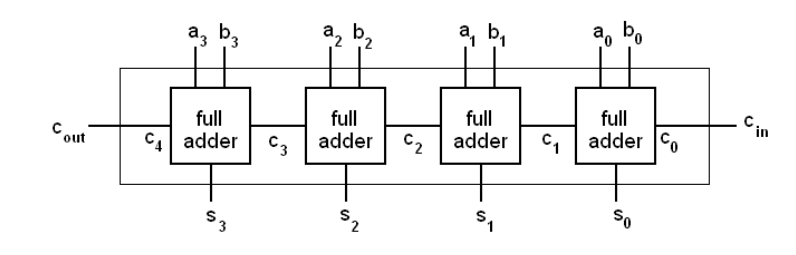
\includegraphics[width=9cm]{./figures/add-6-rc.png}
\end{center}

\subsection{Soustracteur}
Cherchons désormais les équations du soustracteur logique.
\paragraph{Utilisation d'une table de vérité}
On procède de même que précédemment, en écrivant la table de vérité du demi-soustracteur (HS), puis aux équations logiques. Sans surprise, ces équations
ressemblent de très près à celle du demi-additionneur : en numérique aussi, l'addition et la soustraction sont des opérations similaires.
On remarque l'adjonction d'un unique inverseur dans le calcul de la retenue sortante.
\begin{center}
   \begin{minipage}[t]{4cm}
     \vspace{0pt}
     \centering
     \begin{tabular}{|c|c||c|c|}
       \hline
       a & b & D & c \\ \hline
       0 & 0 & 0 & 0    \\ \hline
       0 & 1 & 1 & 1    \\ \hline
       1 & 0 & 1 & 0    \\ \hline
       1 & 1 & 0 & 0    \\ \hline
     \end{tabular}
   \end{minipage}%
   \begin{minipage}[t]{8cm}
     \vspace{5pt}
     \centering
     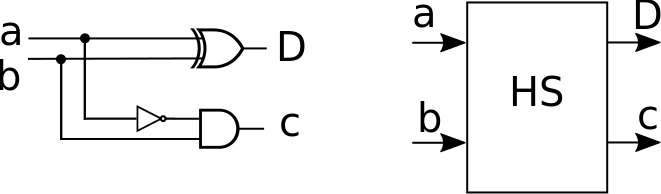
\includegraphics[width=8cm]{./figures/half_sub.png}
   \end{minipage}
\end{center} % added ending }
On pourrait procéder exactement de la même manière que nous l'avons fait pour établir la structure du soustracteur complet. Toutefois, nous n'allons pas
le faire ici, mais passer plutôt à l'utilisation du complément à 2.

\paragraph{Utilisation du complément à 2}
On sait en effet qu'algébriquement on a : $a-b=a+(-b)$. On peut donc voir la soustraction comme une addition de deux nombres dont le second est l'{\it inverse de $b$}.
Attention ! Nous parlons d'"inverse" dans l'algèbre des nombres entiers, mais nous savons désormais (voire le premier chapitre) que $-b$ doit se représenter en complément à 2 en logique
booléenne.
Il faut donc procéder en inversant les entrées $b_i$ et en ajoutant '1' : cet ajout se fait par la retenue entrante, dont on saisit désormais l'intérêt.
\begin{center}
  \centering
  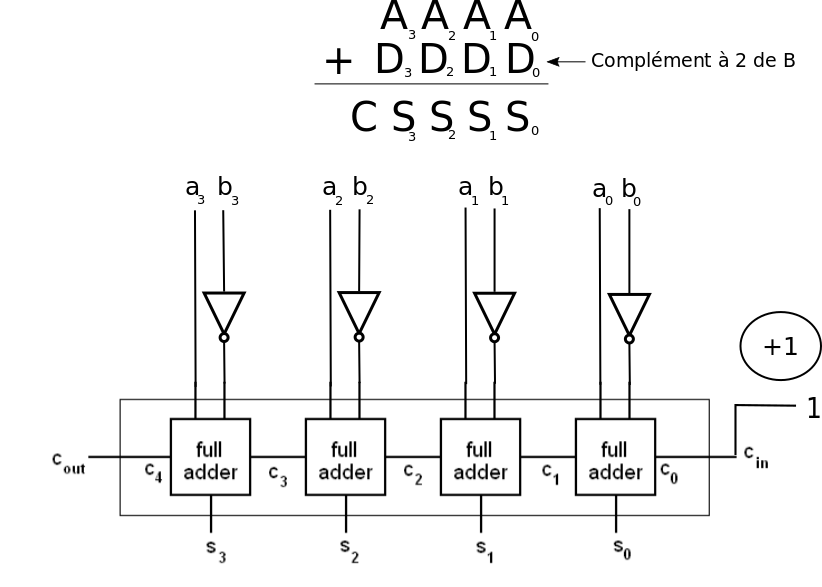
\includegraphics[width=9cm]{./figures/soustracteur.png}
\end{center}


\subsection{Additionneur-soustracteur}
Désormais munis d'additionneurs et de soustracteurs, nous pouvons nous pencher sur d'autres circuits intéressants. Avant d'aborder la mulitplication, étudions l'additionneur-soustracteur.
Comme son nom l'indique,il s'agit d'un circuit capable de réaliser, à volonté, soit l'addition, soit la soustraction. Il s'agit donc par là de notre premier circuit {\it programmable}, qui
nous rapproche au passage d'un ordinateur classique : selon le programme, considéré comme extérieur au processeur (il est stocké dans une mémoire séparée) qui s'exécute, c'est tantôt tel opérateur numérique qui opère, tantôt tel autre.
Dans le cas de l'additionneur-soustracteur, on procède par la même observation que la soustraction précédemment étudiée : quelles entrées $d_i$ dois-je fournir à l'additionneur ?
Dans le cas où je souhaite réaliser l'addition, on doit avoir $d_i=b_i$ (les $a_i$ restent bien évidemment inchangés), alors que pour la soustraction $d_i=\barre{b_i}$, sans oublier l'introduction d'un '1' sur
la retenue entrante.
Pour rendre commandable l'opération, on doit disposer d'une entrée supplémentaire, ici appelée "sub" : quand $sub=1$, le circuit effectuera la soustraction, et l'addition
dans l'autre cas. Etablissons les équations logiques des $d_i$ :
\begin{center}
   \centering
   \begin{tabular}{|c|c||c|}
     \hline
     $b_i$ & sub &  $d_i$ \\ \hline
         0 &   0 &  0    \\ \hline
         0 &   1 &  1    \\ \hline
         1 &   0 &  1    \\ \hline
         1 &   1 &  0    \\ \hline
   \end{tabular}
\end{center}
On voit que l'on a affaire à un magnifique "ou exclusif" ! $$d_i=b_i \oplus sub$$. Le schéma se réduit donc au suivant. Notons que l'introduction du '1' en retenue entrante correspond à la commande "sub".
\begin{center}
  \centering
  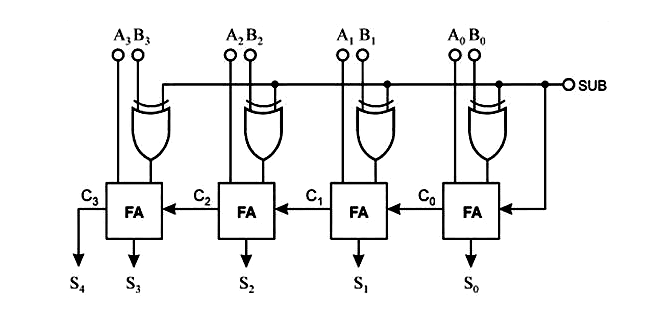
\includegraphics[width=9cm]{./figures/sub-2.png}
\end{center}

\subsection{Multiplieur}
\paragraph{Méthode naturelle}

Pour impléménter un multiplieur en logique combinatoire, il faut simplement comprendre ce qui se passe lorsqu'on "pose" une multiplication traditionnelle et reporter
le principe en respectant la logique booléenne. Le produit de 13 par 11 est donné ici en exemple.

\begin{center}
  \centering
  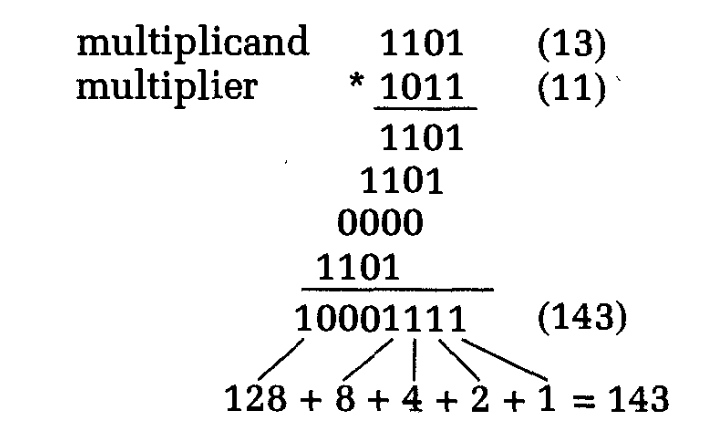
\includegraphics[width=5cm]{./figures/mult-1.png}
\end{center}

On se convainct facilement que la multiplication se réduit, ligne par ligne,
à un conjonction booléenne (et logique). Ligne à ligne, il faut ensuite additionner soit deux opérandes (demi-additionneur), soit trois lorsqu'une retenue est possible (full adder 1 bit).


\begin{center}
  \centering
  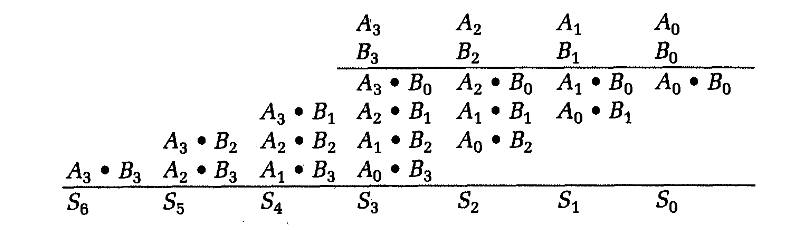
\includegraphics[width=9cm]{./figures/mult-2.png}
\end{center}

Etonnamment, le schéma \footnote{dû à Randu Katz, dont on pourra consulter le livre \cite{katz}} se révèle très irrégulier.

\begin{center}
  \centering
  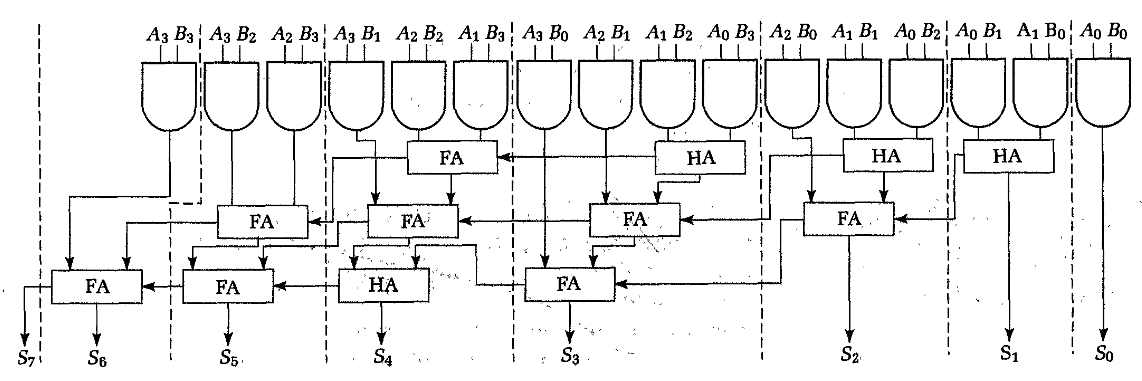
\includegraphics[width=9cm]{./figures/mult-3.png}
\end{center}

\paragraph{Multiplieur avec topologie régulière}
On peut chercher à réaliser un multiplieur, en cherchant un circuit élémentaire "brique de base", que l'on aboute savemment, mais de manière parfaitement régulière, en 2 dimensions. Les microélectroniciens aprécient particulièrement
ce type de circuits, qui se placent facilement sur silicium. Une tel circuit est donné ici à titre de curiosité.

\begin{center}
  \centering
  \includegraphics[width=9cm]{./figures/mult-4.png}
\end{center}

\subsection{Diviseur}
Le diviseur est un peu plus complexe. On repart là aussi de la division classique. Lors du calcul de $A/B$,
on soustrait le diviseur B de manière répétitive aux bits du dividende A, après l'avoir multiplié par '1' ou '0'.
Ce bit de multiplication '0' ou '1' est sélectionné pour chaque étape de soustraction de telle manière que le résultat
de la soustraction n'est jamais négatif. Le résultat est composé des bits de multiplication successifs, alors que
le reste est le résultat de la dernirèe soustraction. Cette algorithme combinatoire peut-être implémenté
comme une série de soustraction. Chaque soustracteur calcule la différence entre 2 nombres en entrée, mais
si le résultat est négatif, l'opération est annulée et remplacée par une soustraction de 0.

\section{Shifter}

\paragraph{Shifter à position fixe}
{\it Shift} signifie "décaler" en anglais. L'opération $f$ consiste à décaler, à droite ou à gauche, les bits $x_i$ de l'unique entrée $x$ présentée en entrée.
Le décalage d'un nombre fixe $\Delta$ de positions est tel que $y_i=f(x_i)=x_{i-\Delta}$. On décale à gauche pour $\Delta>0$ et à droite sinon. Cette opération sur
les seuls indices a la particularité de ne nécessiter {\it aucune} porte logique : il s'agit simplement de prendre un fil d'entrée et
de le connecter sur le bon fils de sortie. C'est une économie en silicium conséquente.

Le shifter à position fixe a notamment la particularité d'être d'une très grande utilité lorsque $\Delta$ est une puissance de 2. En effet,
décaler à gauche (resp. à droite) d'une position $\Delta$ revient à multiplier (resp. diviser) par $log_2(\Delta)$. Par exemple,
pour multiplier un nombre par 2 (resp. par 4,8,16 etc), il suffit, en binaire, de le décaler à gauche d'une position $\Delta=1$ (resp. $\Delta=2,3,4$ etc).
Alors que le multiplieur coûte cher en portes logiques, la cas de la multiplication par de telles puissances de 2 ne coûte rien.
\footnote{Dans le jeu d'instruction d'un processeur, cela a-t-il un intérêt ? La réponse est clairement oui, car il faut parfois plusieurs cycles d'horloges
pour attendre le résultat d'un multiplieur, afin de laisser au multiplieur (éventuellement totalement combinatoire) le temps d'effectuer son calcul.
A l'inverse, le shift est quasi immédiat et ne nécessite donc qu'un seul cycle machine. Nous y reviendrons...}

\paragraph{Barrel shifter}
Lorsque le nombre $\Delta$ n'est pas fixé, mais devient une entrée dur circuit, il faut être à même de décaler "à volonté".
Cette opération plus délicate nécessite un réseau de multiplexeurs.

\section{Multiplexeur}
Le multiplexeur a comme fonction de {\it router} une de ses entrées $e_i$ vers l'unique sortie $f$, en fonction d'une commande $c$.
La commande $c$ indique quelle $e_i$ doit effectivement passer. Mathématiquement cela peut s'écrire : $f(\{e_i,i \in 0..n-1\},c)=e_{c}$.
Il faut donc $\lceil(\log_2{n})$ bits pour constituer le mot de contrôle $c$.
Mais calculons simplement sa table de vérité dans le cas de 2 entrées ($a=e_0$ et $b=e_1$) et d'une commande $c$ (sur un seul bit) :
\begin{center}
   \begin{minipage}[t]{4cm}
     \vspace{0pt}
     \centering
     \begin{tabular}{|c|c|c||c|}
       \hline
       $a$ & $b$ &  c  &  f \\ \hline
       0 & 0 &  0  &  0 \\ \hline
       0 & 0 &  1  &  0 \\ \hline
       0 & 1 &  0  &  0 \\ \hline
       0 & 1 &  1  &  1 \\ \hline
       1 & 0 &  0  &  1 \\ \hline
       1 & 0 &  1  &  0 \\ \hline
       1 & 1 &  0  &  1 \\ \hline
       1 & 1 &  1  &  1 \\ \hline
     \end{tabular}
   \end{minipage}%
   \begin{minipage}[t]{5cm}
     \vspace{5pt}
     \centering
     \includegraphics[width=4cm]{./figures/mux.png}
   \end{minipage}
   \begin{minipage}[t]{5cm}
     \vspace{0pt}
     \centering
     \includegraphics[width=3cm]{./figures/mux2to1.png}
   \end{minipage}
\end{center} % added ending }


Le multiplexeur est un des éléments clés de l'émulation d'une certaine intelligence
par du hardware : il permet de filtrer et d'acheminer des données vers un calcul (ou un élement de stockage), selon le calcul de certains critères transformés
en commandes de ces multiplexeurs. Ils seront logiquement un élément clé de la notion de {\it datapaths} ou "chemins de données", constitutifs de la partie calculatoire
d'un processeur, l'autre partie étant précisément la partie contrôle, et l'ensemble pouvant être interdépendant (un contrôle pouvant dépendre d'un calcul etc).

\paragraph{Crossbar}


\section{Comparateur}
Le comparateur participe souvent aux décisions évoquées à l'instant.

\paragraph{Comparateur 1 bit}
Etudions tout d'abord le comparateur entre 2 entrées $a$ et $b$ codées sur 1 bit.
Calculons les 3 fonctions $<$, $=$ et $>$.
\begin{center}
   \begin{minipage}[t]{4cm}
     \vspace{0pt}
     \centering
     \begin{tabular}{|c|c||c|c|c|}
       \hline
       a & b & $<$ & $=$ & $>$ \\ \hline
       0 & 0 &  0  &  1  & 0   \\ \hline
       0 & 1 &  1  &  0  & 0   \\ \hline
       1 & 0 &  0  &  0  & 1   \\ \hline
       1 & 1 &  0  &  1  & 0   \\ \hline
     \end{tabular}
   \end{minipage}%
   \begin{minipage}[t]{9cm}
     \vspace{-5pt}
     \centering
     \includegraphics[width=8cm]{./figures/comparator-1.png}
   \end{minipage}
\end{center} % added ending }

\paragraph{Comparateur d'égalité de 2 entiers}
Pour passer à une comparaison d'égalité de 2 entiers $a$ et $b$ codés sur $n$ bits, il suffit
de les comparer bit à bit et s'assurer que chacune des comparaisons vaut bien '0'. Cela peut s'écrire :
$$Eq(a,b)=\prod_{i=0}^{i=n-1} a_i \oplus b_i$$
Le circuit dans le cas de $n=4$ est donné sur la figrue suivante.
\begin{center}
  \centering
  \includegraphics[width=6cm]{./figures/comparator-2.png}
\end{center}

\section{Codeurs et Décodeurs}

La fonction d'un codeur est la suivante : il transmet en sortie le code d'un symbole placé en entrée. Généralement ce code
est optimisé et plus simple à transmettre que le symbole initial. Par exemple, à partir de 3 symboles "bleu", "blanc", "rouge", il est
possible de ne transmettre que 2 bits établis au préalable par la fonction de codage : par exemple "00","01","10". A l'inverse, le décodeur
permettra par exemple de n'allumer qu'une des 3 couleurs "bleu", "blanc" et "rouge" à la réception de 2 bits.
\begin{center}
   \begin{minipage}[t]{4cm}
     \vspace{5pt}
     \centering
     \begin{tabular}{|c||c|c|}
       \hline
       couleur & $f_1$ & $f_0$ \\ \hline
       bleu    &    0  &     0 \\ \hline
       blanc   &    0  &     1 \\ \hline
       rouge   &    1  &     0 \\ \hline
     \end{tabular}
   \end{minipage}%
   \begin{minipage}[t]{9cm}
     \vspace{0pt}
     \centering
     \begin{tabular}{|c|c||c|c|c|}
       \hline
       $f_1$ & $f_0$ & bleu & blanc & rouge \\ \hline
          0  &     0 & 1 & 0 & 0 \\ \hline
          0  &     1 & 0 & 1 & 0 \\ \hline
          1  &     0 & 0 & 0 & 1 \\ \hline
          0  &     0 & 0 & 0 & 0 \\ \hline
     \end{tabular}
   \end{minipage}
\end{center} % added ending }

\paragraph{Décodeur 7-segments}
Parmi les décodeurs fréquemment utilisés, on trouve le décodeur 7-segments. Un afficheur 7 segments se présente comme un ensemble de 7 leds a,b,c,d,e,f,g
que l'on peut alumer ou éteindre individuellement. Nous calculerons en TD les 7 équations logiques associées pour les nombres hexadécimaux allant de 0 à 15.
\begin{center}
  \centering
  \includegraphics[width=6cm]{./figures/afficheur-7seg.png}
\end{center}

\section{Conclusion}
Ce chapitre a permis de nous familiariser avec un certain nombre de fonctions combinatoires usuelles. Leur caractère combinatoire s'est manifesté par le fait qu'à aucun moment, il n'a été nécessaire, au cours
des calculs menés, de se référer au passé des signaux en présence. Le calcul s'est toujours réalisé des entrées vers les sorties, sans retour possible.
Parmi les fonctions combinatoires intéressantes, l'arithmétique figure en bonne place. Souvenons nous que c'est bien par ces procédés que nous sommes en mesure
d'utiliser un matériau (le silicium ici) pour calculer ! Il faut savoir que le domaine de l'arithmétique sur silicium est un domaine toujours actif. Il est notamment
toujours à l'honneur dans le domaine de la cryptographie et des télécommunications en général.
On complètera la lecture de ce chapitre par la consulation d'autres ouvrages comme \cite{mano},\cite{clements}.

\chapter{Circuits séquentiels}

\minitoc
%====================================================
\section{Introduction}
Nous sommes désormais armés pour représenter et manipuler les nombres sous forme binaire (chapitre 2), puis les traiter par une électronique numérique (chapitre précédent).
Toutefois, les opérateurs étudiés jusqu'ici se bornaient à des traitements combinatoires. En aucune manière, nous ne nous sommes autorisés jusqu'ici à prendre
en compte des valeurs du passé. En particulier, {\bf il nous est interdit de reboucler un signal sur le nuage combinatoire dont il est issu}.
Par exemple, il nous est jusqu'ici impossible de réaliser directement un circuit qui réalise une suite numérique comme : $$u_{n}=u_{n-1}+42,n \in  \mathbb{N}^+$$

Les circuits que nous allons considérer désormais sont appelés circuits {\it séquentiels}.
Nous nous intéressons ici, précisément à l'indice des suites précédentes : on considère que les indices successifs représentent des instants logiques discrets.
Pour parler de la valeur précédente du signal $u_n$, nous devons nous doter d'un moyen électronique de franchir un nombre de "pas temporels".
Par la suite, nous parlerons de "cycles" (ou "coup d'horloge") plutôt que de "pas temporels".
Ainsi, dans la suite précédente, il existe un cycle entre entre $u_n$ et $u_{n-1}$. C'est donc une seconde discrétisation --celle du temps-- qui nous préoccupe ici, après celle qui consistait à discrétiser les valeurs d'un signal.
Ces circuits, qui sont à même de se référer à des valeurs du passé, sont des circuits {\it séquentiels}.

\section{Discrétiser le temps}

\paragraph{Eviter la "cacophonie"}

Les circuits combinatoires précédents se présentent sous la forme d'un nuage : ses comportements sont, d'un point de vue microscopique, très complexes à analyser. Ainsi, si l'on
disposait d'un oscilloscope suffisamment précis, on constaterait un très grand nombre d'événements (ou "oscillations" ou "changement de valeurs") {\it internes} fluctuants dans le temps et donc d'une mesure à l'autre.
\begin{center}
  \includegraphics[width=12cm]{./figures/cloud-complexe-events.png}
\end{center}


De même, aux bords du circuit, sur les entrées-sorties, ces événements apparaissent au gré des stimulations extérieures (générateurs de signaux, capteurs, etc), parfaitement {\it asynchrones} : par ce terme
"asynchrone", on indique qu'il n'existe pas a priori de référentiel temporel qui puisse donner un "tempo" commun à tous.
Nous cherchons donc ici à trouver un moyen d'éviter cette cacophonie qui semble se profiler, et toutes les tracasseries d'ingénieurs qui lui
seraient liées. On observe d'ores-et-déjà qu'il semble suffire d'attendre un temps "suffisamment long" pour que le signaux se stabilisent et que les
sorties délivrent leur résultat attendu. Une fois que l'on est sûr que ce temps long est respecté, l'ordre interne qui a mené au résultat final n'importe plus.

\paragraph{Notion d'horloge périodique}
Le moyen technique de créer de l'ordre dans la succession des évènements d'un circuit est de recourir à une horloge commune.
Cette horloge est ici un signal carré, parfaitement périodique, de période $T$. Là encore, l'analogie musicale s'impose : à la manière d'un chef d'orchestre, l'horloge vise à donner un rythme unique et commun à tous les éléments en présence.
Il serait  possible de préciser le ratio entre le temps du signal à '1' et à '0', mais comme nous allons le voir ceci n'est pas d'un grand intérêt : en effet, au sein de ce signal carré, nous allons
uniquement nous intéresser au {\it front montant} de cette horloge. Idéalement, ce front montant peut être vu comme instantané. Par analogie avec les mathématiques du traitement du signal,
l'ensemble des fronts montants peut être vu comme un {\it peigne de Dirac} parfait, ou "shah" de Dirac \footnote{Toutefois, même si cette référence mathématique
est intéressante, elle a ses limites et n'est guère référencée par les Electroniciens. La raison en est simple : en général les traiteurs de signaux font une hypothèse algorithmique
forte qui consiste à supposer que le signal est {\it disponible}, dans son intégralité, au moment du calcul. L'Electronicien quant à lui s'inquiète plus de la manière de capter et traiter ce flux, souvent à la volée ({\it streaming})}.
\begin{center}
   \begin{minipage}[t]{4cm}
     \vspace{0pt}
     \centering
     $$\Sh(t)=\sum_{n=-\infty}^{n=+\infty}\delta(t-nT_e)$$
   \end{minipage}%
   \begin{minipage}[t]{8cm}
     \vspace{20pt}
     \centering
     \includegraphics[width=6cm]{./figures/shah_dirac.png}
   \end{minipage}
\end{center} % added ending }

\section{Bascule D}
La bascule D est l'élément clé de notre discrétisation du temps. C'est le seul élément électronique sensible au front montant de l'horloge. La bascule D n'est donc pas une "nouvelle porte logique",
mais a un status particulier et un fonctionnement particulier. Néanmoins, il est d'usage de présenter sa table de vérité, en analogie avec les portes logiques. Alors que les entrées
d'une table de vérité classique font apparaître des valeurs logiques, ici la table fait intervenir le front montant.\\
\begin{center}
   \begin{minipage}[t]{8cm}
     \vspace{0pt}
     \centering
     \includegraphics[width=8cm]{./figures/d-ff-infos.jpg}
   \end{minipage}
\end{center} % added ending }
La fonction basique de cette bascule D est de réaliser une copie de son entrée 'D' sur sa sortie 'Q'. Cette copie a lieu sur le front montant de l'horloge. Il faut physiquement
un très court temps de propagation entre le signal d'horloge et la sortie, appelé "clock-to-Q". Ce temps physique est à prendre en compte à un moment ou un autre,
mais n'oublions pas notre but initial de nous "dépolluer" de toute préoccupation d'ordre "physique", pour nous concentrer sur la réalisation mathématique de notre suite numérique (discrète).
La fonction de copie semble donc bien modeste. Elle assure pourtant la distinction entre une valeur "avant" et une valeur "après" le front montant d'horloge. En dehors
de ce bref instant d'échantillonnage, la bascule D conserve la valeur précédemment échantillonnée.

\subsection{Fonction d'échantillonnage de la bascule D. Set-up et hold. Metastabilité.}
Une première utilisation intéressante de la bascule D est qu'elle permet d'échantillonner un signal d'entrée qui varie de manière plus rapide que l'horloge.
Pour que cet échantillonnage se passe correctement, la bascule doit être utilisée dans des conditions particulières : notamment, il est nécessaire que le signal (numérique)
à échantillonner soit {\it stable} un peu avant et un peu après le front montant. Ces deux temps à respecter s'appelle respectivement le temps de {\it set-up} et de {\it hold}.
Si par mégarde ou malchance, le signal d'entrée fluctue précisément à cet instant, la bascule entre dans un état particulier dit {\it métastable}. Cet état ne permet
pas de garantir avec certitude que le bon '0' ou le bon '1' apparaîtront en sortie de la bascule. Pire, cette sortie peut même se mettre à fluctuer sans sembler pouvoir
se stabiliser.

\begin{center}
  \includegraphics[width=6cm]{./figures/dff-chrono.png}
\end{center}

\subsection{Décalage temporel : la raison d'être de la bascule D}
La véritable raison d'être de la bascule est qu'elle permet de décaler un signal d'entrée d'un cycle d'horloge : le signal Q ne pourra en effet être "vu" d'un calcul en aval qu'au
cycle d'horloge qui suit.

\begin{center}
  \includegraphics[width=9cm]{./figures/DFF_decalage_temporel_timed.png}
\end{center}

\section{Quelques {\it patterns} de conception synchrone}

Tout système numérique, simple ou complexe, est une combinaison de portes logiques et de bascules D.
Un tel assemblage générique est présenté sur la figure suivante : on observe un enchaînement de traitements
combinatoires et de bascule D. Des rebouclages peuvent exister, mais il doit forcément exister une bascule D sur les chemins
concernés : aucune chemin bouclé sur lui même ne peut être purement combinatoire. Ce schéma générique peut être décliné dans une
très grande variétés de patterns de conception. Le pattern le plus étudié est probablement les automates d'états finis ("FSM" : finite state machine), auquels
nous consacrons le chapitre suivant.

\begin{center}
  \includegraphics[width=10cm]{./figures/synchrone.png}
\end{center}

Pour l'heure, on peut citer quelques autres circuits numériques connus, qui font usage de la bascule D \footnote{En Informatique théorique , l'importance des automates est telle
que ces circuits électroniques sont vus comme de automates particuliers. L'Electronicien ne fera pas cet amalgamme.}.

\subsection{Registre à décalage}
Les registres à décalage sont des assemblages linéaire de bascule D, chaînées les unes à la suite des autres. Lorsqu'une donnée se présente, la précédente est déjà
dans le premier étage, et l'avant-dernière dans le deuxième étage etc. A chaque front montant d'horloge, de manière synchrone, toutes les bascules prennent leur entrée et modifient
leur sortie Q, {\it en même temps}. C'est une forme primitive de traitement parallèle. A titre de curiosité, la simulation logicielle d'un tel dispositif n'est pas immédiate ; il faut doubler
le nombre de variables et calculer dans un premier temps les {\it états futurs} de toutes les bascules, puis, dans un second temps,  réaliser la mise à jour de toutes les variables.
Le décalage synchronisé de ces registres est fascinant et confine à l'harmonie. Toutefois, on ne peut manquer de faire la comparaison avec le travail à la chaîne : le taylorisme, né
dans l'industrie de l'automobile s'en est grandement inspiré (voir "les temps modernes" de Charlie Chaplin) !


\begin{center}
  \includegraphics[width=6cm]{./figures/Shift_Register.png}
\end{center}

\subsection{LFSR : linear feedback shift register}
Les LFSR ont l'intérêt de créer de manière simple des suites en apparence aléatoires. En réalité, les suites
de valeurs produites sont pseudo-aléatoires et parfaitement récurrentes à partir d'un certain rang. La simplicité
des LFSR les rendent malgré tout très attrayants dans de nombreuses situations. Noter la présence d'un ou plusieurs OU exclusifs, qui
sont les véritables "créateurs de désordre" au sein de la suite. La place de ces Xor peut être définie à l'aide de polynômes générateurs.
\begin{center}
  \includegraphics[width=9cm]{./figures/lfsr.png}
\end{center}

\subsection{Bascule D et multiplexeur : mémorisation}
La seule fonction de décalage semble très éloignée des fonctions que l'on peut attendre d'un processeur numérique. De fait,
la bascule D est le plus souvent utilisée conjointement à un multiplexeur. Ce multiplexeur (combinatoire) permet de sélectionner
à volonté l'action d'{\it échantillonner ou non} : le signal de contrôle du multiplexeur permet effectivement soit de router le signal vers l'entrée D de la bascule, soit
de refaire circuler la donnée précédemment stockée dans la bascule, au coup d'horloge précédent. On parle effectivement de {\it recirculation} de la donnée Q, qui tourne
en boucle de la sortie, vers l'entrée etc : la donnée est ainsi piégée. Ce piégeage est une {\it mémorisation}. Très souvent, ce mécanisme est présenté comme
intégré au sein de certaines bascules, tant il est commun : le signal de contrôle du multiplexeur s'appelle alors un {\it enable}. Lorsque l'enable est à '1',
la donnée présentée en entrée est effectivement échantillonnée, sinon, c'est la valeur précédente qui reste "occupe" la bascule.

\begin{center}
  \includegraphics[width=5cm]{./figures/dff-enable.png}
\end{center}


\subsection{Compteurs et timers}
La fonction d'un compteur est d'incrémenter un registre. Cet incrément peut se faire sur tous les 'top' d'horloge, ou de manière commandée en utilisant un signal d'autorisation.
Les compteurs peuvent notamment servir à réaliser des {\it timers} : ces dispositifs très importants en embarqué permettent d'interrompre un circuit au bout d'un certain temps. Ce temps
correspond à la valeur limite d'un compteur. L'intérêt de ces timers est par exemple de laisser un processeur réaliser une fonction principale, et de le détourner périodiquement vers une tâche annexe : c'est la notion
d'{\it interruptions}.

\begin{center}
   \begin{minipage}[t]{8cm}
     \vspace{0pt}
     \centering
     \includegraphics[width=6cm]{./figures/compteurs.png}
   \end{minipage}

   \begin{minipage}[t]{8cm}
     \vspace{0pt}
     \centering
     \includegraphics[width=6cm]{./figures/timer.png}
   \end{minipage}

\end{center} % added ending }


%====================================================
\section{Initialisation d'une bascule D}
Les symboles précédents des bascules D sont incomplets ; deux signaux importants n'y figurent pas, à savoir : le signal "set" et le signal "reset".
Ces signaux interviennent au tout démarrage du circuit, à sa mise sous tension : ce temps particulier s'appelle la phase de {\it reset du circuit}.
A cet instant particulier (qui dure quelques millisecondes), il est nécessaire de placer toutes les bascules D dans un état connu ('0' ou '1'), bien maîtrisé.
Cette mise sous tension provient d'une action extérieure (appui sur le bouton de la télé, etc), qui prendra fin pour laisser place au régime permanent.
Le signal "set" sert à initialiser la sortie Q de la bascule à '1', tandis que le signal "reset" place cette sortie Q à '0'. Cette prise en compte
est {\it asynchrone} : les signaux "set" et "reset" sont prioritaires sur l'horloge. Après la phase de reset, c'est le régime permanent qui s'établit :
l'horloge reprend alors "tous ses droits" et est la seule à commander la valeur de la sortie Q (recopie de D). Ce régime permanent est généralement
considérablement plus long que le régime transitoire de reset. Si, pour une raison ou une autre, les signaux de set ou reset sont à nouveau
utilisé, ils reprendront instantanément la "main" sur la sortie Q, et imposeront une nouvelle sortie Q. Mais encore une fois, le schéma classique
de fonctionnement est : phase de reset suivi d'un très long régime permanent.

\begin{center}
  \includegraphics[width=7cm]{./figures/d-ff-full.jpg}
\end{center}

Pour bien mettre en oeuvre la phase de reset, on peut observer les équations d'implication suivantes, qui résument le mécanisme d'initialisation :
\begin{itemize}
  \item $set=POL_s \implies Q=1$
  \item $reset=POL_r \implies Q=0$
\end{itemize}
Elles font intervenir un couple ($POL_s,POL_r$). POL dénote la {\it polarité} sur set ou du reset, placé en indice. La polarité indique quelle est la valeur
logique active : par exemple si $POL_s=0$, cela signifie qu'il faudra produire un $0$ sur le signal set pendant le démarrage, pour que que l'on obtienne
l'effet escompté sur $Q$, à savoir $Q=1$. Notons que sauf exception, on a $POL_s=POL_r$.
La polarité est également signalée sur les schémas par un petit cercle (présent ou absent) près du signal set ou reste de la bascule : la présence du cercle
indique une polarité à '0' et '1' en cas d'absence.
Lors du régime permanent, il faudra s'assurer que les signaux set et reset n'ont aucune influence sur $Q$ et donc
qu'ils sont bien commandés. S'ils sont commandés avec une valeur différente de leur polarité, ils n'auront aucun effet. Lors de la conception, il
faut donc s'assurer que l'on relie correctement les boutons de reset à ces signaux, avec les bonnes polarités : par exemple, il faudra se poser la question
concernant l'appui sur le bouton : cet événement produit-il une tension à '0' ou à '1' ? Et quelle est la polarité des signaux de reset de la bascule ?

\paragraph{Exemples}
Nous donnons ici deux exemples (voir schémas) impliquant 2 bascules D et un signal de reset arrivant de l'extérieur. Supposons que l'on cherche à initialiser les bascules dans l'état $Q_1=0$ et $Q_0=1$.
On suppose que le signal de reset est actif haut : lorsqu'on appui sur le bouton de reset, le signal devient '1'. Lorsqu'on le relache, il repasse à '0'. Pour initialiser les bascules,
 il faut jouer sur les signaux set et reset des 2 bascules : cela fait 4 signaux à connecter de manière appropriée. Aucun signal ne doit rester non connecté (aucun signal "en l'air").
 \begin{itemize}
   \item Dans le cas du schéma de gauche, la solution consiste d'une part à connecter le signal reset à l'entrée reset de la bascule $Q_1$ et au set de la bascule $Q_0$. Les autres entrées des bascules doivent être connectées, même si elles sont inactives : il suffit
   de les connecter à la masse (0).
   \item Dans le cas du schéma de droite, il faut adapter la polarité du signal de reset (actif haut) pour activer correctement le reset de la bascule (présence d'un cercle $\implies$ polarité à 0).etc
 \end{itemize}


 \begin{center}
   \includegraphics[width=8cm]{./figures/dff_init.png}
 \end{center}

\paragraph{Simplification grâce aux HDL}
Le mécanisme de reset peut être perçu comme relativement complexe. Qu'on se rassure : les langages de descriptions matérielle, dont VHDL (étudié plus loin),
masque totalement ce travail de fourmi consistant à réaliser ces câblages minutieux.

%=====================================================
\section{Conclusion}
Ce chapitre nous a permis de nous doter de l'élément clef des systèmes séquentiels, à savoir la bascule D. Nous avons pris le parti de ne pas "ouvrir le capot" de la bascule D, alors
que c'est souvent ce que s'empresse de faire de nombreux manuels. Les raisons en sont multiples : d'une part les HDL reposent uniquement sur la synthèse de bascules D ; d'autre part, sous le capot
de ces bascules, plusieurs types de structures peuvent apparaître, la plus connue étant la bascule RS asynchrone. C'est un montage tête-bêche de 2 portes logiques NOR (ou NAND) : la sortie de l'une est câblée sur l'autre et l'ensemble
présente un cycle combinatoire que nous avons tenté de totalement exclure (règle de base : pas de boucles combinatoire en conception numérique !). A notre sens, ces deux seules raisons, associées à un temps d'apprentissage court (6 à 7 séances !)
autorisent de tels sauts conceptuels.

\chapter[Machines d'états finis]{Automates\\ {\it Machines d'états finis}}
\minitoc
%====================================================
\section{Introduction}
Parmi les circuits séquentiels précédemment évoqués, les automates ont une place privilégiée. Ces automates, appelés également
{\it machines d'états finis} ou encore {\it FSM (finite state machines)} permettent d'élaborer des circuits très complexes, de manière
simple et systématique. Par ailleurs, les automates sont un objet d'étude à part entière pour les informaticiens théoriciens, qui les utilisent
comme support à la modélisation de systèmes, y compris lorsque du logiciel prédomine dans ces systèmes : fondamentalement, tout système informatique
peut être considéré comme un (très gros) automate. Cette base conceptuelle solide pour les Electroniciens et les Informaticiens l'est aussi -- sans surprise-- pour les Automaticiens.
Les automates sont essentiels aux
systèmes embarqués : ils assurent à la fois la notion de séquencement ainsi que les tâches de contrôle
de dispositifs. Dans un premier temps, nous reviendrons sur des rappels concernant ces automates.
Dans un second temps nous calculerons les équations logiques constitutives de ces FSM.

\section{Machines d'états finis}
Il y a lieu de distinguer deux types d'automates : Moore et Mealy. Très proches conceptuellement, il est toutefois nécessaire de
bien comprendre leurs différence pour l'Ingénieur Numéricien. Nous verrons notamment que le couplage de tels automates peut-être source
de tracasseries délicates.

\paragraph{Automate de Moore}

Une automate de Moore est un sextuplet $(Q, \Sigma, \Delta, \sigma, \lambda, q_0 )$ :
\begin{itemize}
\item $Q$ est un ensemble fini d’états, $q_0$ est l’état initial
\item $\Sigma$ est l’alphabet d’entrée, $\Delta$ est l’alphabet de sortie
\item $\delta$ est une application de $Q \times \Sigma $ dans $Q$
\item $\lambda$  est une application de $Q$ dans $\Delta$, donnant la sortie associée à chaque état
\end{itemize}

La sortie de l'automate de Moore en réponse à une entrée $a_1 a_2\dots a_n$ , $n \geq 0$ est
$\lambda(q_0),\lambda(q_1)\dots \lambda(q_n)$ où
$q_0 ,\dots, q_n$ est la séquence d’états tels que $\lambda(q_{i-1},a_i) = q_i$ pour $1 \leq i \leq n$.
Remarque: Un automate de Moore retourne la sortie $\lambda(q_0)$ pour toute entrée.

\paragraph{Automate de Mealy}

Une automate de Mealy est un sextuplet $(Q, \Sigma, \Delta, \sigma, \lambda, q_0 )$ :
\begin{itemize}
\item $Q$ est un ensemble fini d’états, $q_0$ est l’état initial
\item $\Sigma$ est l’alphabet d’entrée, $\Delta$ est l’alphabet de sortie
\item $\delta$ est une application de $Q \times \Sigma $ dans $Q$
\item $\lambda$  est une application de $Q\times \Sigma$ dans $\Delta$, donnant la sortie associée à chaque état
\end{itemize}

$\lambda(q, a)$ donne la sortie associée à une transition d’un état q sur l’entrée a.
La sortie de l'automate de Mealy,en réponse à une séquence d’entrées $a_1,\dots a_n$ est
$\lambda(q_0, a_1) \lambda(q_1 , a_2 ) \dots \lambda(q_{n-1}, a_n)$
où $q_0 , q_1 ,\dots, q_n$ est la séquence des états tels que
$\lambda(q_{i-1}, a_i) = q_i$ pour $1 \leq i \leq n$.

\begin{figure}[h!]
  \centering
  \includegraphics[scale=0.25]{./figures/moore_mealy.png}
  \caption{Automates de Moore et de Mealy}
  \label{fig:mealy_moore}
\end{figure}

\paragraph{Comparaison}
Les deux définitions sont très proches l'une de l'autre. On doit seulement comprendre que dans le cas d'une machine de Mealy, les sorties
dépendent des entrées et de l'état courant, alors que dans le cas de la machine de Moore, ces sorties dépendent uniquement de l'état courant.
En règle générale, les machines de Mealy sont plus rapides : leur chemin critique est plus court. Par contre, elles sont souvent proscrites des
bonnes règles de conception --en vigueur dans la plupart des sociétés-- car elles peuvent induire des bugs difficiles à localiser. En effet,
l'interconnexion de plusieurs automates de Mealy peut présenter des cycles combinatoires. On rappelle que ces cycles (ou boucles) combinatoires
sont interdites en logique synchrone car elle ne permettent pas de déterminer la fréquence propre de l'horloge du circuit.\\

En règle générale, toutefois, on plus code naturellement avec des machines de Mealy. La seule chose à prendre en compte est de bien clore le chemin
des sorties combinatoires par un registre adéquat. Cela fait partie des bonnes règles applicables par ailleurs : les entrées et les sorties d'un circuit
un tant soit peu complexe doivent être "clockées", c'est-à-dire échantillonnées dans des registres.

% \begin{figure}[h]
%   \centering
%   \includegraphics[scale=0.4]{./figures/comb_loops_mealy.png}
%   \caption{Composition d'automates de Mealy et risque de cycles combinatoires}
%   \label{fig:mealy_loops}
% \end{figure}

\paragraph{Exemple}
Nous présentons sur la figure \ref{fig:fsm} un exemple de FSM décrite à l'aide de bascule (ici une seule) et de portes logiques.
Les deux fonctions clés y sont représentées à savoir : la fonction d'état suivant et la fonction de sortie.
Malheursement, imaginer, concevoir, analyser et réaliser des automates à ce {\it niveau de détail} est sujet à erreur.
Par la suite, nous allons plutôt passer, {\it au préalable}, par une représentation plus adéquate, sur laquelle nous allons nous appuyer pour
établir les équations. Cette représentation est graphique ; nous l'appelerons "diagramme à bulles" ou diagramme états-transitions.
Elle est expliquée dans le paragraphe suivant. En TD, nous recoderons l'exemple \ref{fig:fsm} en diagramme états-transitions.
\begin{figure}[h]
  \centering
  \includegraphics[scale=0.4]{./figures/fsm-ex1.png}
  \caption{Exemple d'un automate matériel, réalisé à l'aide de portes logiques et (ici) d'une bascule D. En TD, nous tenterons de répondre à la question suivante : quel est le diagramme états-transitions équivalent ?}
  \label{fig:fsm}
\end{figure}

\section{Diagramme états-transitions}
Dans cette représentation graphique, un état est dénoté par un cercle, alors que les transitions sont représentées par
des flêches qui joignent les cercles. Il y a donc un état source et un état transition. Les transitions sont annotées par une expression booléenne qui indique la condition de changement d'état. Concernant les états, on indique
généralement le nom de l'état à l'intérieur du cercle (ou toute indications permettant de distinguer les états entre eux). Il existe également un état de démarrage, dénoté par un double cercle (ou parfois cible d'une flèche sans source).
L'automate évolue d'un état à l'autre, mais peut également réaliser des actions qui peuvent avoir lieu sur les transitions (Mealy) ou directement dans les états (Moore). Ces actions sont marquées ici après la double barre oblique.

\paragraph{Exemple : vending machine}
La figure \ref{fig:vending_machine} présente un automate appelé "vending machine". C'est un automate qui gère la délivrance d'un produit (soda, etc). Il se présente sous la forme d'un diagramme
états-transitions à 5 états. L'environnement immédiat de cet automate est un ensemble de capteurs et d'actionneurs. Ces derniers peuvent également se présenter sous la forme d'automates, de telle
sorte que c'est un ensemble complexe d'automates communicants qui constitue le système numérique complet. La FSM commande lé mécanisme de délivrance par deux signaux "open" et "close". Le mécanisme
de délivrance possède également un {\it timer} interne, non représenté ici qui décompte le temps à partir du moment où un ordre d'ouverture a été donné : lorsque le temps de délivrance (quelques secondes par exemple)
s'est écoulé, le signal "top" est à '1'. La FSM centrale est donc également sensible à cette entrée du mécanisme, de sorte que l'ensemble apparait comme bouclé.

\begin{figure}[h]
  \centering
  \includegraphics[scale=0.3]{./figures/vending_machine.png}
  \caption{Vending machine et son environnement}
  \label{fig:vending_machine}
\end{figure}

\section{Consistance ou {\it causalité} d'une machine d'états finis}

Pour que la FSM résultante soit considérée comme correcte ou ``consistante'', on doit examiner les
 transitions $c_i(s)$ partant de chaque état $s$ :
\begin{itemize}
\item \textbf{Réactivité} Les conditions sur les transitions doivent être {\it collectivement exhaustives} : il existe forcément une transition à '1'.
$$\forall s \in S : \sum_i c_i(s)=1$$
\item \textbf{Déterminisme} Les conditions sur les transitions doivent être {\it mutuellement exclusives} : on ne peut pas avoir deux transitions à '1' en même tem
ps.
$$\forall s \in S, \forall (i,j), i\neq j : c_i(s).c_j(s)=0$$
\end{itemize}

Cela signifie simplement que dans un état, il existe un, et un seul, état suivant.
Un tel automate, réactif et déterministe, est dit {\it causal}. Notons qu'un état peut avoir comme état suivant lui-
même : dans ce cas, le système décrit ne change pas d'état, tout simplement. \\

\section{Encodage des états}
Le diagramme états-transitions est une abstraction graphique qui est d'une grande aide lors de la conception amont.
Notamment, on a abstrait les états grâce à une simple bulle et un nom parlant ("symbolique"). Lors de la réalisation
concrète en Electronique, il faudra substituer cet état symbolique par un certain nombre de bascules qui "stockent" les bits d'états.
Il faut donc établir une correspondance (bijective) entre ces symboles et les codes binaires de ces états. Cette
correspondance s'appelle l'encodage des états. Là encore, il existe plusieurs manières de réaliser cet encodage.

\paragraph{Encodage dense}
L'encodage le plus naturel consiste à numéroter chacune des états en présence, pris dans un ordre arbitraire. La valeur binaire du numéro d'un état est
précisément le code de l'état. Cette manière de procéder conduit à une encodage dit "dense". Le terme "densité" utilisé
s'explique par le fait que le nombre de bascules résultant est restreint : pour $n$ états symboliques, on obtient
$\lceil \log_2(n) \rceil$ bascules. Observons le cas de la FSM "vending machine", et un encodage dense choisi. Pour 5 états
distincts, on a ici 3 bits d'états ; la densité est ici toute relative puisqu'avec 3 telles bascules, on pourrait encoder
jusqu'à 8 états.

\begin{table}[!htbp]
  \centering
  \begin{tabular}{|l|c|c|}
        \hline
        état  & numéro & code binaire  \\ \hline \hline
        Idle  & 0      & 000           \\ \hline
        Got5  & 1      & 001           \\ \hline
        Got10 & 2      & 010           \\ \hline
        Got15 & 3      & 011           \\ \hline
        Wait5 & 4      & 100           \\ \hline
    \end{tabular}
\end{table}

\paragraph{Encodage one-hot}
L'encodage {\it one-hot} ou, en français, "un bit par état", consiste à associer à chaque état d'une FSM de $n$ états
symbolique un code de $n$ bits de longueur. Cet encodage est de ce fait bien moins intuitif que l'encodage dense précédent.
Les bits d'un code "one-hot" sont particuliers : dans ce code, un seul bit est à '1' (tous les autres à '0'). Un exemple
d'un tel encodage est donné dans le tableau suivant.

\begin{table}[!htbp]
  \centering
  \begin{tabular}{|l|c|c|}
        \hline
        état  & numéro & code binaire  \\ \hline \hline
        Idle  & 1       & 00001           \\ \hline
        Got5  & 2       & 00010           \\ \hline
        Got10 & 4       & 00100           \\ \hline
        Got15 & 8       & 01000           \\ \hline
        Wait5 & 16      & 10000           \\ \hline
    \end{tabular}
\end{table}


\paragraph{Compromis temps-surface}

L'intérêt de l'encodage "one-hot" tient à la simplicité de conception des automates qui en découle.
Nous allons y revenir très bientôt. De plus les équations logiques des transitions, qui découleront, se révêlent plus simples (moins de portes logiques) et présentent
des chemins critiques plus courts que dans le cas de l'encodage dense.
Toutefois, étant donné le nombre plus important de bascules D engendrées dans le cas de l'encodage "one-hot",
il faudra calculer soigneusement les gains éventuels lors de l'attribution définitive de l'encodage.
En effet, on considère qu'une bascule D correspond à environ 10 portes logiques à 2 entrées (typiquement une porte AND). Ce nombre
peut notamment se révéler prohibitif en comparaison du nombre de portes engendrées dans le cas d'un encodage dense.
De même, signalons que ce seul encodage dense (et d'ailleurs tout encodage) est un choix, qui peut avoir des conséquences
insoupçonnées en ce qui concerne la simplification des équations qui en découleront. C'est un problème très complexe, qui a mobilisé
un grand nombre d'études théoriques jusque dans les années 1990.
Ce calcul est désormais automatisé dans les outils de synthèse, sous la forme d'heuristiques.

%====================================================
\section{Méthode générale de conception d'un automate}
On cherche à établir les équations logiques de l'automate : les équations logiques de la fonction état suivant,
ainsi que de la fonction de sortie. On doit établir une {\it table de vérité séquentielle} qui, à partir d'une présentation de l'ensemble des combinaisons de l'état courant et des entrées,
recense toutes les sorties, mais également l'état futur du système.On suggère ici de procéder en 2 étapes.

\paragraph{Table de vérité symbolique}
  La première consiste à conserver le nom {\it symbolique} des états tandis que la seconde fait a
pparaître l'{\it encodage} de ces états.

\begin{table}[!htb]
  \centering
  \begin{tabular}{|c|c|c|c||c|c|c|c|}
        \hline
        état courant & entrée 1 & ... & entrée n &  état suivant & sortie 1 & ... & sortie n \\ \hline
        IDLE        & ~    & ~     & ~            & ~            & ~        & ~   & ~    \\ \hline
        \dots       & ~    & ~     & ~            & ~            & ~        & ~   & ~    \\ \hline
        GOT5        & ~    & ~     & ~            & ~            & ~        & ~   & ~    \\ \hline
        \dots       & ~    & ~     & ~            & ~            & ~        & ~   & ~    \\ \hline
    \end{tabular}
\end{table}

%\FloatBarrier
\paragraph{Table de vérité explicite}

Cette énumération conduit donc à un nouveau tableau, encore plus explicite, où figurent, {\it à gauche}, les sorties $Q_i$ des bascules
--c'est l'état couran du système-- et, {\it à droite} les entrées $D_i$ de ces mêmes bascules. Pour établir cette
table de vérité séquentielle, on énumère toutes les valeurs possibles de la partie de gauche, et on calcule les sorties et les $D_i$.


\begin{table}[!htb]
  \centering
    \begin{tabular}{|c|c|c|c|c|c||c|c|c|c|c|c|}
        \hline
        $Q_n$ & \dots & $Q_0$ &  entrée 1 & ... & entrée n & $D_1$ & \dots & $D_0$ & sortie 1 & ... & sortie n \\ \hline
        ~   & ~    & ~  & ~  & ~  & ~  & ~  & ~  & ~        & ~   & ~ & ~        \\
        ~   & ~    & ~  & ~  & ~  & ~  & ~  & ~  & ~        & ~   & ~ & ~        \\
        \hline
    \end{tabular}
\end{table}

\section{Exemple complet}
Illustrons notre propos avec la FSM exposée sur la figure. Il s'agit d'un automate de de Moore car on constate que la sortie $f$ a lieu dans les états, et non sur les transitions.

\begin{figure}[h]
  \centering
  \includegraphics[scale=0.4]{./figures/exo_fsm.png}
  \caption{Tableaux de Karnaugh de l'exemple}
  \label{fig:karnaugh}
\end{figure}

\paragraph{Encodage}
La FSM présente 3 états. Choisissons un encodage dense :
\begin{table}[!htbp]
  \centering
  \begin{tabular}{|l|c|c|}
        \hline
        état  & numéro & code binaire  \\ \hline \hline
        S0  & 0       & 00           \\ \hline
        S1  & 1       & 01           \\ \hline
        S2  & 2       & 10           \\ \hline
    \end{tabular}
\end{table}

\paragraph{Table de vérité symbolique}
Passons à la table de vérité. On reporte les observations du schéma précédent.
\begin{table}[!htb]
  \centering
  \begin{tabular}{|c|c||c|c|}
        \hline
        état courant & e &  état suivant & f \\ \hline
        S0 & 0 & S0 & 0 \\ \hline
        S0 & 1 & S1 & 0 \\ \hline
        S1 & 0 & S1 & 1 \\ \hline
        S1 & 1 & S2 & 1 \\ \hline
        S2 & 0 & S2 & 1 \\ \hline
        S2 & 1 & S0 & 1 \\ \hline
    \end{tabular}
    \caption{Table de vérité avec nom explicite des états.}
    \label{fig:thruth_1}
\end{table}

\paragraph{Table de vérité avec encodage explicite}
Il en découle la table de vérité suivante.
\begin{table}[!htb]
  \centering
    \begin{tabular}{|c|c|c||c|c|c|}
        \hline
        $Q_1$ & $Q_0$ &  e & $D_1$ & $D_0$ & f \\ \hline
        0 & 0 & 0 & 0 & 0 & 0 \\ \hline
        0 & 0 & 1 & 0 & 1 & 0 \\ \hline
        0 & 1 & 0 & 0 & 1 & 1 \\ \hline
        0 & 1 & 1 & 1 & 0 & 1 \\ \hline
        1 & 0 & 0 & 1 & 0 & 1 \\ \hline
        1 & 0 & 1 & 0 & 0 & 1 \\ \hline
        1 & 1 & 0 & x & x & x \\ \hline
        1 & 1 & 1 & x & x & x \\ \hline
    \end{tabular}
    \caption{Table de vérité avec encodage explicite}
    \label{fig:thruth_1}
\end{table}

\paragraph{Tableaux de Karnaugh et Equations logiques}
On établit les 3 tableaux de Karnaugh, relatifs aux équations des 2 bascules et de la sortie. On effectue les regroupements simplificateurs, en profitant
des valeurs {\it don't care} 'X', que l'on peut positionner à '0' ou '1' de manière à créer des regroupements plus intéressants.
\begin{center}
\includegraphics[scale=0.4]{./figures/exemple_table_k.png}
\end{center}

% \begin{figure}[h]
%   \centering
%   \includegraphics[scale=0.35]{./figures/exemple_table_k.png}
%   \caption{Tableaux de Karnaugh de l'exemple}
%   \label{fig:karnaugh}
% \end{figure}

Les équations obtenues, sont :
\begin{align}
 D_0 & = Q_0.\barre{e}+\barre{Q_1}.\barre{Q_0}.e \\
 D_1 & = Q_1.\barre{e}+Q_0.e \\
 f   & = Q_1 + Q_0 \\
\end{align}

\paragraph{Circuit électronique}
Le circuit réalisant l'automate exemple est donné sur la figure \ref{fig:circuit}. Notons qu'afin de ne pas surcharger le schéma, nous avons omis les fils
relatifs à l'initialisation des bascules D, ainsi que l'horloge.
\begin{figure}[h]
  \centering
  \includegraphics[scale=0.35]{./figures/fsm_circuit.png}
  \caption{Implémentation matérielle de l'automate}
  \label{fig:circuit}
\end{figure}


\section{Gérer la complexité }
\paragraph{Position du problème}

On se rend compte que le nombre d'entrées dans cette table de vérité grandit très vite : on se souvient alors que pour $n$ entrées, on devra avoir $2^n$ lignes d'énumérations
des combinaisons dans cette table. Cela ne devient plus gérable par un humain. Il faut automatiser.
Notons que le nombre précédent $2^n$ est indépendant du nombre des sorties ; la complexité des équations booléennes de ces sorties croît en fonction de $n$, ce qui n'est guère
rassurant : on pourra  avoir $2^n$ monômes dans ces équations. Bref : il faudra le plus souvent se résoudre à recourir à des synthétiseurs automatiques pour le calcul des équations ou recourir à des statégies plus intelligentes
que le calcul "brute force". Généralement, il est judicieux d'{\it observer} les relations qui existent entre les contraintes booléennes.

\paragraph{Contraintes mutuelles}

Ainsi, prenons le simple cas du dé électronique (dé à jouer, à 6 points maximum) : on verra en TD que ce dé peut être modélisé par une FSM. Pour simuler l'effet d'un dé qui est lancé, on appuie
sur un bouton. Pendant que le bouton est enfoncé, une FSM allume et éteint les diodes correspondant aux points du dé, en comptant de 1 à 6.
Avec une horloge dont la fréquence de fonctionnement est élevé, le joueur ne peut évidemment pas voir ce défilement. Lorsqu'il relâche le bouton, un chiffre est figé sur les points.
Logiquement, on s'attend à ce que l'on ait à établir 6 équations logiques : une équation par diode. On remarque toutefois que tous les points qui s'allument et s'éteignent
sur une face du dé sont interdépendants et des "symétries" apparaissent dans les équations. Ceci conduit à ne pas traiter 6 équations, mais
seulement quelques unes d'entre elles, les autres en découlant facilement. Nous garderons donc en mémoire qu'il faut un peu d'observation et de perspicacité pour traiter de tels
problèmes.

\section{Méthode particulière : cas de l'encodage {\it one-hot}}

\paragraph{Intuition} Il existe un cas particulier d'encodage qui permet d'éviter totalement la méthode générale précédente : l'encodage {\it one-hot}. Posons nous
la question de la signification de cet encodage : nous savons qu'il est appelé "un bit par état". Cela signifie qu'à un instant donné, une seule bascule
aura une sortie $Q_i$ à '1' ; nous connaissons donc instantanément, du fait de cette seule observation, dans quel état on se trouve.
Nullement besoin d'observer les autres valeurs (à '0') des autres bascules. On dit que la bascule en question est "allumée" lorsque sa sortie vaut '1' .
Si on observe désormais le fonctionnement de l'automate durant plusieurs coups d'horloges, on verra successivement s'allumer différentes bascules,
{\it l'une après l'autre} : tout se passe comme si un jeton se déplaçait d'une bascule à l'autre. Lorsque la bascule $i$ détient le jeton, l'automate se trouve dans l'état de numéro $i$ !



\paragraph{Obtention directe des équation} On peut utiliser les propriétés de cet encodage pour établir une correspondance {\it directe} entre le schéma initial et le circuit correspondant.
Dit autrement : il suffit d'observer le diagramme états-transitions de l'automate pour construire directement le circuit !
Pour cela, il suffit d'établir des règles simples :

\begin{itemize}
  \item On dessine une bascule $D$ pour un état $S$
  \item Pour chacune des transitions sortantes d'un état $S_i$ vers un état $S_j$, on dessine une porte AND connectée d'une part à la sortie $Q$ de la bascule de l'état $S_i$, et
  d'autre part la condition booléenne $c$ de la transition $S_i\rightarrow_{c} S_j$. Appelons $c_{i,j}$ la sortie de cette porte AND.
  \item Pour chacune des transitions entrantes d'un état $S_j$ on dessine une porte OR connectée à l'entrée $D_j$ et possédant autant d'entrées qu'il existe de transitions entrantes.
  A partir des états précedents $S_i$, on connecte le signal $c_{i,j}$ sur une des entrées de cette porte OR.
\end{itemize}

\begin{figure}[!htb]
  \centering
  \includegraphics[scale=0.3]{./figures/one_hot_method.png}
  \caption{Procédé simplifiant la génération d'un circuit d'automate dans le cas d'un encodage {\it one-hot}.}
  \label{fig:one_hot}
\end{figure}

Ce schéma de traduction est très simple à mettre en oeuvre. Il est résumé sur la figure \ref{fig:one_hot} : on se borne à regarder le schéma et réécrire
les équations logiques des entrées $D_i$. Voici un exemple, sur la figure \ref{fig:one_hot2}.

\begin{figure}[!hbt]
  \centering
  \includegraphics[scale=0.25]{./figures/fsm_one_hot.png}
  \caption{Exemple pour la méthode directe d'obtention des équations, à partir de l'encodage one-hot}
  \label{fig:one_hot2}
\end{figure}

Les équations sont directement obtenues :
$$
\begin{array}{lcl}
  D_1 & = & Q_1.a+Q_2.\overline{b}.\overline{c}\\
  D_2 & = & Q_2.(b+c)+Q_1.\overline{a}\\
\end{array}
$$

\section{A propos du caractère fondamental des automates}

Nous l'avons déjà mentionné : les automates sont des objets étudiés par différentes
communautés scientifiques. C'est un objet fondamental de l'Informatique, car il permet
de raisonner sur les évolutions temporelles d'un système : les automates sont à l'Informaticien (et l'Electronicien)
ce que les équations différentielles sont au Physicien. A titre d'illustration, observons le schéma de la figure \ref{sys1}. Cette figure décrit l'architecture d'un système-sur-puce (SoC : system-on-chip).
Un SoC est l'agglomération d'un ensemble de composants {\it sur un seule et même puce}. Généralement un processeur y tient un rôle central. Il est en communication
avec des périphériques de communication (clavier, écrans, ethernet), mais également des périphériques d'accélération de calculs le plus souvent dédiés. Cette
communcation s'effectue à travers un bus (et de plus en plus, à travers un NoC réseau-sur-puce). La complexité de l'ensemble est difficile à appréhender pour un humain.


\begin{center}
\begin{minipage}[t]{10cm}
 \centering
 \includegraphics[width=10cm]{./figures/system_1.png}
 \label{sys1}
\end{minipage}
\end{center}

\paragraph{} Toutefois, in fine, l'ensemble de ces éléments constitutifs ne représentent {\it que} des automates, comme l'illustre la figure suivante.
Ce socle est suffisamment solide pour que des outils dits de {\it verification formelle} permettent de vérifier les propriétés du système dans son ensemble.

\begin{center}
\begin{minipage}[t]{10cm}
 \centering
 \includegraphics[width=10cm]{./figures/system_2.png}
\end{minipage}
\end{center}

\section{Conclusion}
Ce chapitre nous a permis de découvir la notion d'automate matériel.
L'implémentation matérielle de tels automates peut être réalisée de manière quasi-mécanique, en mobilisant nos connaissances
en matière de logique combinatoire, tableaux de Karnaugh, mais également bascules D. Nous avons également abordé la notion de consistance
de ces automates : un calcul formel permet de s'assurer que notre automate a du sens. Ce calcul se fait au préalable de la réalisation
concrète du circuit. C'est là une propriété intéressante, liée à la logique booléenne, que l'on ne retrouve guère en matière logiciel. Là, le domaine
du matériel semble en avance sur le logiciel : notons toutefois qu'une classe de languages informatiques, dédiés à la réalisation de logiciels embarqués,
s'appuie sur les mêmes calculs et les mêmes raisonnements formels pour assurer la fiabilité des logiciels embarqués. Ces langages s'appellent {\it langages synchrones} : on comprend
désormais bien cette appellation ! Je vous invite notamment à lire, voir ou écouter les conférences de Gérard Berry, à l'Académie des Sciences.
Il illustre parfaitement, mieux que quiconque, ce propos.

\chapter[VHDL]{Langages de description matérielle\\{\it L'exemple de VHDL}}
\minitoc

\section{Avant propos}
\lettrine{C}e chapitre est une introduction à VHDL. Ce langage sera étudié et utilisé plus en détail en deuxième année. Plusieurs
cours universitaires découplent totalement l'enseignement de l'Electronique numérique et celui de VHDL (ou Verilog). C'est une
démarche qui a du sens : elle permet notamment de raisonner sur les concepts de l'Electronique, avant de s'engouffrer dans les
particularismes de tel ou tel langage. Toutefois, notre expérience nous laisse penser qu'il est frustrant de s'arrêter si près
d'expériences possibles, simples et concrètes, qui permettent au futur ingénieur de mieux se projeter dans ce domaine passionnant
que sont les systèmes embarqués numériques. Nous avons donc choisi une {\it approche intermédiaire} qui consiste à se limiter à un survol
de VHDL, {\it restreint à cette seule UV 1.2 de l'ENSTA Bretagne}. Nous nous bornerons :

\begin{itemize}
  \item A la description de systèmes d'équations booléennes sous la forme d'{\it assignations concurrentes} de VHDL.
  \item A la description de bascule D sous la forme de {\it processus "clockés"}
  \item A la description de quelques bancs de test (testbench) qui illustrent la démarche de vérification par simulation.
\end{itemize}

Cette restriction laisse de côté les aspects les plus productifs de VHDL et notamment la maîtrise de la notion d'inférence au niveau transfert
de registres (RTL). Cela sera étudié de manière poussée en deuxième année. Les plus impatients pourront consulter différentes ouvrages \cite{chu_rtl}, \cite{chu_fpga}.
Dans les flots de conception traditionnels, notre restriction correspond stricto-sensu au niveau logique.

\section{Introduction : les langages de description matérielle}

\paragraph{Naissance de VHDL}

La Silicon Valley est née de l'essor qui a suivi l'invention du transistor (1947). Diverses sociétés concevant
des circuits à base de semi-conducteurs ont commencé à échanger des informations concernant la structure et le comportement temporel de circuits. On a rapidement compris
que les simples dessins ne suffisaient pas : la description des circuits requiert des langages spécifiques. Il s'agit des HDL ou "hardware description languages".
Au niveau analogique, c'est SPICE qui s'est imposé : il permet de décrire des assemblages de composants tels que des diodes, resistances, capacités, etc sous la forme d'une netlist textuelle.
Très rapidement, la nécessité d'un format commun de {\it description} des circuits numériques s'est également imposée. Le DARPA (Département à la Défense américain) a initié en 1981 la création
de VHDL. IBM, Intermetrics et Texas Instrument ont pris le projet en main. La syntaxe de VHDL s'est fortement inspirée d'ADA, un langage informatique généraliste et très prometteur à l'époque. C'est finalement en 1987 que l'IEEE publie un premier standard mondial,
amendé en 1993. Différentes évolutions ont eu lieu depuis, et des groupes de travail continuent de s'activer autour de l'évolution du langage. L'ambition du langage --initialement cantonné
à la description de circuits-- s'est étendue : il a été rapidement possible de simuler, puis de synthétiser des circuits décrits en VHDL. En parallèle, un autre langage aux buts similaires est né :  Verilog, inventé pour la simulation logique par la société Gateway Design Automation,
puis commercialisé par la société Cadence, qui reste un des leaders mondiaux de l'EDA (Electronic Design
Automation). Verilog est également un standard IEEE désormais. A noter que plus tard, d'autres langages de description matérielle ont vu le jour : on pense notamment à SystemC, qui élève le niveau d'abstraction
au dessus de ce qu'il est possible décrire en VHDL ou Verilog.
Ce domaine de la description et de la modélisation de systèmes numériques reste très actif : ces outils de simulation et de synthèse sont la clé de voûte de toute l'Industrie du Semiconducteur.

\paragraph{Particularités de VHDL : deux sémantiques}

VHDL est un langage très exigeant en terme de syntaxe, réputée verbeuse (mais explicite) mais également en terme de "sémantique" : outre le fait qu'il est fortement typé, il possède
en réalité 2 sémantiques très différentes en ce qui concerne le {\it temps}. D'une part, il sert à la simulation sur ordinateur : la signification d'un programme VHDL est donc imposée par ce simulateur, qui doit
représenter le parallélisme final du circuit à l'aide d'un algorithme séquentiel. D'autre part, il sert à la synthèse de circuits qui existeront in fine, sur silicium. Le concepteur
en VHDL doit donc en permanence "jongler" avec ce qui est limité à la simulation et ce qui devra subir le flot de synthèse. La prise en compte de cette dualité nécessite beaucoup d'expertise.

\paragraph{Démarche de modélisation}
Ecrire des programmes VHDL nécessite d'adhérer à une démarche de modélisation très différente de l'écriture de programmes traditionnels (Python, Java, C etc). Comme leur nom l'indique,
les HDL sont utiles à la {\it description} de circuits : il est inutile d'écrire des programmes VHDL en imaginant qu'il correspondront "par miracle" à une circuit. Il faut avoir à l'inverse
le circuit sur papier ou tout au moins bien en tête, avant de se lancer dans sa description. Le modèle séquentiel des langages cités précédemment laisse {\it peut-être} l'opportunité de
programmer "au fil de l'eau" : ce n'est pas le cas ici. Dans notre utilisation de VHDL dans cette UV, il s'agit d'abord d'obtenir les équations logiques, puis de les transcrire en VHDL.
Ce sera également le cas en deuxième année, mais on se situera à un niveau d'abstraction (RTL) plus confortable que ces simples équations logiques : il existe des construction du langage
qui nosu affranchissent de l'écriture explicite des équations. Mais nous respectons ici le partie-pris pédagogique de restriction du langage.


% \section{Aperçu du flot de conception}
% \paragraph{Processus}
% Le {\it flot de conception} est le processus qui organise la création des systèmes numériques, mais aussi de leur vérification. Ce processus
% enchaîne un grand nombre d'étapes que nous nous sommes efforcés de simplifier ici. Chaque étape s'accompagne de ses propres techniques, outils et langages.
% Ces flots commencent très en amont, avec par exemple des réflexions en terme de marketing (quel est le besoin du marché, etc). On dégage de ces réflexions des spécifications de plus en plus précises.
% Ces spécifications peuvent être d'ordre algorithmique (fonctionnelles) ou englober des spécifications dites {\it non-fonctionnelles} : par exemple les dimensions
% de la future puce, sa consommation, sa compatibilité électromagnétique, etc. Ces spécifications aboutissent généralement à un plan
% d'ensemble de ces fonctions, interconnectées par des canaux de communications. Les langages comme VHDL peuvent intervir dès ces phases amont, jusqu'à des phases
% très avancées de réalisation. Ces canaux peuvent être plus ou moins
% abstraits, c'est-à-dire dont le détail n'est pas encore à portée de main.
% L'ingénieur cherche à rendre ces spécifications {\it exécutables}. Il cherche par là à s'assurer au plus tôt, par simulation,
% que l'ensemble du futur système répond aux exigences initiales. Ce modèle du système encore abstrait s'appelle un {\it prototype virtuel}.
% Toutefois, force est de constater que  l'ingénieur cherche
% généralement à se reposer au plus tôt sur des standards de communications entre fonctions : il s'agit de bus connus comme AMBA, AXI, Wishbone,etc.
% Il fait le plus souvent office, pour le flot aval, de {\it modèle de référence}, aussi appelé en anglais "golden model". C'est un modèle qu'on ne remettra
% guère en cause et qui permettra de {\it vérifier} que le comportement du circuit final (ou de tout intermédiaire) à bien le comportement
% attendu aux entrées-sorties.
%
% \paragraph{Testbenches}
% C'est par simulation que la vérification précédente s'effectue. Pour simuler un système numérique, il faut imaginer une véritable "paillasse" de
% laboratoire : ce laboratoire est également virtuel, dans le sens où les instruments n'existent pas physiquement, mais sont simulés. Par exemple,
% il sera nécessaire de simuler l'existence d'un générateur d'horloge ou autres générateurs de signaux spécifiques. De même, on devra
% brancher des sondes également virtuelles, des oscilloscopes, et des générateurs de fichiers. Dans le flot basé sur VHDL, tous
% ces "instruments" sont en réalité des composants VHDL plus ou moins abstraits. Nous verrons quelques exemples de tels codes.

\section{La structure globale d'un programme VHDL}

Les programmes que nous allons écrire présentent une structure systématique :
\begin{enumerate}
  \item Déclaration de \textbf{librairies} et de \textbf{packages} utilisés
  \item \textbf{Entity} : c'est la description des entrées-sorties du circuit, et de paramètres génériques éventuels (taille des données etc).
  \item \textbf{Architecture} : description de l'organisation interne du circuit.
\end{enumerate}
Ces déclarations apparaissent généralement dans cet ordre, dans un seul et même fichier. Notons que ce n'est toutefois pas une obligation : par exemple, une entité et son architecture
peuvent être décrites dans des fichiers séparés. Il s'agit d'{\it unités de compilation} : le compilateur VHDL est capable de les compiler individuellement et de les assembler au final.

\subsection{Déclaration de librairies et packages}
Un exemple est donné ici. Il fait appel à deux librairies fournies par l'IEEE. Ces librairies sont incontournables.
\begin{itemize}
  \item La librairie \textbf{std\_logic\_1164} permet d'utiliser les types les plus standard de VHDL, à savoir le type std\_logic et le type std\_logic\_vector.
  Ce sont simplement l'incarnation du "bit" et d'un ensemble de bits, mais cette librairie permet de bénéficier d'autres valeurs que '0' et '1'. Ces autres valeurs sont d'une grande aide lors de la simulation du circuit et
  permettent de trouver au plus tôt des cas litigieux.
  En pratique, il est par exemple intéressant de pouvoir savoir si un fil est effectivement piloté ou non par une tension : dans le cas où aucune tension ne pilote le fil,
  on affaire à une tension 'u' (unknown). Cette valeur apparait en simulation lorsque le concepteur a oublié de connecter ("driver") le fil (signal) concerné. De même, le concepteur
  a peut-être connecté deux sources sur un même fil :  ce dernier est alors en conflit (valeur 'x'). Ce dernier cas survient lorsque deux ou plusieurs sources tentent d'imposer leur tension. De même une équipotentielle peut se trouver dans un état de haute impédance (valeur 'z').
  Le type bit existe nativement (sans appel à des librairies) dans VHDL, mais n'est guère utilisé, car il a la faucheuse tendance de masquer les non-connexions précédentes ou les conflits.
 \item  La librairie \textbf{numeric\_std} : c'est la librairie qui nous permet entre autre de faire des calculs sur des nombres signés ou non signés. Le type std\_logic\_vector précédent
 n'autorise pas d'emblée ce type de calculs arithmétiques (c'est un tableau sans arithmétique associée). Un ensemble de conversions très utiles sont également disponibles dans cette librairie.
\end{itemize}

\lstset{basicstyle=\small,language=VHDL}
\begin{lstlisting}[frame=single]
  librairie ieee;
  use ieee.std_logic_1164.all;
  use ieee.numeric_std.all;
\end{lstlisting}


\subsection{Notion d'entité}
L'entité permet de décrire les \textbf{ports} d'entrées-sorties du circuit, ainsi que d'éventuels paramètres dit "génériques". C'est l'\textbf{enveloppe extérieure} du composant.
Pour être correctement utilisée, cette entité devra être instanciée en respectant ces entrées-sorties : il faudra venir connecter des \textbf{signaux} à ces ports.

Un premier exemple de description d'entité est donné ici, sans paramètre.
\lstset{language=VHDL}
\begin{lstlisting}[frame=single]
  entity example1 is
     port(
       reset_n      : in  std_logic;
       clk          : in  std_logic;
       a            : in  std_logic;
       b,c,d        : in  std_logic;
       data1,data2  : in  std_logic_vector(31 downto 0);
       data3,data3  : in  unsigned(7 downto 0);
       f            : out std_logic;
       dataout      : out std_logic_vector(15 downto 0)
     );
  end entity;
\end{lstlisting}
Cette entité présente un \textbf{nom} ("example1"), puis un ensemble de \textbf{ports}, qui sont des entrées ("in") ou des sorties ("out"). Notons qu'il existe aussi
le moyen de décrire des ports bidirectionnels ("inout"), qui ne seront pas décrits ni utilisés ici ; ils nécessitent des buffers trois-états. On remarque immédiatement
la syntaxe exigeante de VHDL, avec la présence de nombreuses parenthèses, signes de ponctuations (";",",")  et certaines redondances dans l'utilisation des mots clés ("entity").
Les bons éditeurs de textes comme Emacs fournissent une aide substantielle dans l'écriture du VHDL, en offrant des auto-complétions puissantes, voire la génération de gabarits (squelettes de
code ) complets, déclenchées sur des racourcis claviers.

\subsection{Notion d'architecture}
L'architecture est le contenu réel du circuit. Si l'entité était un capot de voiture, l'architecture représente le moteur, sous le capot.
Une architecture est explicitement associée à une entité unique. Notons par contre qu'une entité peut être associée à plusieurs architectures : cela restitue l'idée que derrière l'apparence externe d'un composant (derrière l'entité), on peut
trouver plusieurs organisations différentes, de la même manière que derrière un capot de voiture de course, on peut trouver soit un moteur performant, soit un un moteur plus banal etc.

\begin{lstlisting}[frame=single]
  architecture logique of example1 is
    -- ici les declarations necessaires a l'architecture :
    -- ...signaux notamment.
    signal w1 : std_logic;
    -- etc...
  begin
    -- ici le contenu effectif
  end logique;
\end{lstlisting}

Dans l'exemple donné, le nom de l'architecture est "logique" (choix évidemment libre), et le nom de l'entité associée est "example1".
L'architecture est elle-même structurée : une première partie permet de placer les déclarations locales à l'architecture. Le corps véritable de l'architecture se
situe entre les mots clés "begin" et "end". Noter que le "end" est suivi du nom de l'architecture.

\section{Les éléments clés de l'architecture}
C'est dans le corps de cette architecture que le concepteur peut réelement décrire son circuit en détail. Plusieurs nouveaux concepts sont mis à disposition, associés
à des éléments de syntaxe que nous allons détailler. La chose importante à comprendre est qu'au sein de cette architecture, l'ordre d'écriture de ces concepts
n'a pas d'importance : ceci diffère de ce que vous avez l'habitude d'écrire (python, java, etc). Ceci restitue pourtant naturellement l'idée de {\it décrire} le circuit
(imaginé, dessiné ou plus rarement existant), à la manière d'un naturaliste qui décrirait un fleur en se laissant le droit de commencer par la tige, les racines ou les pétales.
\subsection{Assignations concurrentes des signaux}

Les assignations concurrentes s'effectuent sur des {\it signaux} : une assignation est la manière d'affecter un signal. Un signal peut être vu comme un fil (une équipotentielle).
Les assignations s'effectuent en {\it parallèle} : en conséquence, un ensemble d'assignations concurrentes peuvent être vues comme un ensemble de définitions d'équations. Leur ordre n'a pas d'importance, ce qui
tranche avec la notion d'assignation de variable dans un programme impératif classique. Dans l'exemple
qui suit, la partie de droite de 'affectation du signal $w1$ est une expression booléenne. Dans la seconde assignation, la partie droite est plus complexe car elle est conditionnelle, mais in fine,
le synthétiseur logique synthétisera 8 équations logiques (une pour chaque fil du signal $w2$), après avoir {\it inféré} un réseau booléen constitué d'un additionneur, d'un multiplieur 8 bits et de multiplexeurs.

\begin{lstlisting}[frame=single]
  architecture logique of example1 is
    signal w1 : std_logic;
    signal w2 : unsigned(7 downto 0);
  begin
    -- ici deux assignations concurrentes

    w1 <= (a or b) and c;

    w2 <= (a+b) when cmd="00" else
          (a*b) when cmd="01" else
          to_unsigned(0,32);

  end logique;
\end{lstlisting}

\subsection{Processus}
Une autre manière d'effectuer des actions parallèles, qui figure dans le corps d'une architecture, est le recours aux {\it processus}. Un processus est un "bout de code", évalué de manière séquentielle par le simulateur.
Vous pouvez ainsi décrire des "programmes" séquentiels qui s'exécutent en parallèle et interagissent : leur moyen d'interagir est d'affecter des signaux. Le signal peut être vue comme des canaux de communication entre processus.
Une des grandes difficultés de VHDL est que ces processus, {\it évalués} de manière séquentielle par le simulateur, peuvent être utilisés à la description de dispositifs électroniques qui ne sont pas forcément séquentiels.
Ainsi, selon l'écriture, un processus résultera, après traitement par le synthétiseur, en un circuit combinatoire ou séquentiel. Etudions quelques exemples, afin de nous permettre d'y voir plus clair.

% BUG for ! : without escaping !!!!!!!!!!!!!!!!!!!!!!!!!!!!!!
\paragraph{Exemple 1 \: processus générant un circuit combinatoire}
Nous allons décrire le même circuit que précédemment, à l'aide d'un seul processus.

\begin{lstlisting}[frame=single]
 p1 : process(a,b,c)
 begin
   w1 <= (a or b) and c;
   w2 <= 1;
 end process;
\end{lstlisting}

Il s'agit  du même exemple que précédemment codé avec des assignations concurrentes. Le concepteur a la choix de la forme
qu'il utilise pour décrire son futur circuit. Ce processus (précédé d'un label optionnel --ici "p1"--), est structuré comme un programme séquentiel : chaque instruction du processus est d'ailleurs suivi d'un ";", marqueur traditionnel de séquentialité
dans les langages comme C ou Java. On y retrouve un "if"..."elsif". Le simulateur (lui-même séquentiel) profitera de cette forme séquentielle pour simuler aisément le circuit ; le simulateur calcule par contre
qu'aucun temps physique significatif ne s'est ici écoulé entre les instructions au début du processus et celles de la fin. Le synthétiseur, quant à lui, est capable d'inférer un matériel parfaitement combinatoire.
Ces deux manières de voir le processus sont ainsi cohérentes.

\paragraph{Exemple 2 \: processus générant un circuit séquentiel}
Exemple :
\begin{lstlisting}[frame=single]
architecture ex2 of circuit is
  signal d1,d2,q : std_logic;
begin
  p1 : process(clk)
  begin
    if rising_edge(clk) then
      q1 <= a;
    end if;
  end process;

  p2 : process(reset_n,clk)
  begin
    if reset_n='0' then
     q2 <= "000";
    elsif rising_edge(clk) then
      if enable='1' then
        q2 <= b;
      end if;
    end if;
  end process;

end logique;
\end{lstlisting}

Dans cet exemple, le concepteur a cherché à décrire deux bascules D, à l'aide de 2 processus. Le {\it principe fondamental} pour comprendre l'inférence de bascules D est le suivant :
\begin{center}
  \fbox{\begin{minipage}{0.9\textwidth}
     \textbf{Toute assignation d'un signal, sous la condition d'un front d'horloge, résulte en une bascule D}.
  \end{minipage}}
\end{center}


\paragraph{Exemple 3 : processus utilisé en banc de test}
Les processus sont également utilisés pour simuler des environnement de tests : ils peuvent décrire des générateurs de signaux, ou à l'inverse des instruments d'observation de signaux. Ces
processus ne servent que dans des {\it bancs de test virtuels} (testbench) sur lesquels nous allons revenir. Ces processus n'ont pas alors vocation à être synthétisable, et l'on peut donc
utiliser pleinement le langage VHDL. On qualifiera ces processus de "comportementaux".

Dans l'exemple suivant, on décrit la génération d'un signal (ou "stimulus"), à l'aide d'une processus qui opère sur plusieurs cycles d'horloge

\begin{center}
   \begin{minipage}[t]{9cm}
     \vspace{0pt}
     \begin{lstlisting}[frame=single]
     architecture bhv of circuit is
       signal s : unsigned(7 downto 0);
     begin
       stimulus : process(clk)
       begin
         s <=x"00";
         report "waiting for reset";
         wait until reset_n='1';
         for i in 0 to 10 loops
           wait until rising_edge(clk);
         end loop;
         report "starting sequence";
         s <= x"0A";
         wait until rising_edge(clk);
         s <= x"0B";
         wait until rising_edge(clk);
         s <= x"0C";
         wait until rising_edge(clk);
         s <= x"00";
         report "done."
         wait; --forever
       end process;

       -- autres processus ...

     end logique;
     \end{lstlisting}
  \end{minipage}%
  \begin{minipage}[t]{6cm}
   \vspace{40pt}
   \centering
   \includegraphics[width=5cm]{./figures/chronogramme.png}
  \end{minipage}
  \end{center} % added ending }
\subsection{Instanciation de composants et d'entités}
L'instanciation consiste à utiliser un modèle de circuit, précédemment décrit. Sans cette instanciation, un couple entité-architecture ne peut être simulé : il n'est pas "incarné", mais reste un modèle imaginé.
Une analogie naturelle peut être faite avec la programmation orientée objet, qui distingue bien la notion de {\it classe} et d'{\it objets} (appelés "instances"). Il faut dans notre cas imaginer
que l'on dispose d'une réserve infinie de composants sur étagère,et que l'on vient construire un système en les "posant" sur une table imaginaire. Cette table imaginaire est l'architecture associée à une entité :
l'instanciation se fait donc en parallèle des assginations concurrents vues précédemment. Elle permet en outre de construire des circuits hiérarchiques, à la manière des poupées russes (ou poupées gigognes) : un composant
peut être composé de composants etc...

Deux formes d'instanciations sont possibles : l'instanciation de {\it component} et l'instanciation d'{\it entity}. Une fois posés, ces composants devront être connectés aux signaux
en présence : horloge, reset, entrées, sorties, signaux locaux. Cette connection s'appelle le "port map". Comme nous allons le voir, il existe là aussi deux formes de port map : explicite ou positionnel.

\paragraph{Instanciation de composants}
La première forme a tendance a disparaître des pratiques, car elle requière notamment plus de texte : au sein de l'architecture receptacle, il est nécessaire de rappeler l'interface de l'entité, sous la forme
d'un "component". Supposons que l'on dispose d'un modèle entité-architecture d'un circuit "PGCD", dans un fichier "pgcd.vhd". Pour instancier ce circuit, il est nécessaire de procéder comme suit explicité dans
l'exemple.

\begin{lstlisting}[frame=single]
architecture bhv of circuit is

  component MonCircuit is
    port(
      reset_n      : in  std_logic;
      clk          : in  std_logic;
      a,b          : in  std_logic_vector(31 downto 0);
      f            : out std_logic_vector(31 downto 0);
    );
  end component;

  signal aa,bb, f1,f2 : std_logic_vector(31 downto 0);

begin -- instanciation de 2 composants

  -- port map explicite, de la forme :
  --    port formel => signal
  inst_1: MonCircuit
    port map (
      reset_n => reset_n,
      clk     => clk,
      a       => aa,
      b       => bb,
      f       => f1
    );

  -- port map positionnel
  inst_2: MonCircuit
    port map (reset_n,clk,aa,bb,f2);

end bhv;
\end{lstlisting}

\paragraph{Instanciation d'entités}

L'instanciation d'entité est syntaxiquement voisine, mais plus succinte, puisque nous n'avons pas à déclarer l'existence d'un "component", comme c'était le cas
précédemment.

\begin{lstlisting}[frame=single]
architecture bhv2 of circuit is

  signal aa,bb, f1,f2 : std_logic_vector(31 downto 0);

begin -- instanciation d'une entite

  inst_1: entity work.MonCircuit(RTL)
    port map (
      reset_n => reset_n,
      clk     => clk,
      a       => aa,
      b       => bb,
      f       => f1
    );

end bhv2;
\end{lstlisting}


\section{Décrire des machines d'états finis}

\subsection{FSM au niveau logique}
{\bf Nous restreignons ici le style de description à l'UV1.2}. D'autres styles de descriptions des FSMs, plus légers, seront vus en 2ième année, et sont évoqués dans la section suivante.

Comme étudié au chapitre précédent, on peut désormais décrire des FSMs à l'aide des seuls concepts d'équations logiques et de bascule D. Nous proposons le code VHDL de l'automate dont nous avons
précédemment trouvé les équations.

\begin{lstlisting}[frame=single]
library ieee;
use ieee.std_logic_1164.all;

entity FSM is
 port(
     reset_n : in std_logic;
     clk     : in std_logic;
     e       : in std_logic;
     f       : out std_logic
   );
end FSM;

architecture logic of FSM is
 signal q0,q1,d0,d1 : std_logic;
begin

  -- description des bascules d'etat
  state: process(reset_n,clk)
  begin
    if reset_n='0' then
      q0 <= '0';
      q1 <= '0';
    elsif rising_edge(clk) then
      q0 <= d0;
      q1 <= d1;
    end if;
  end process;

  -- next state logic :
  d0 <= (q0 and not(e)) or (not(q1) and not(q0) and e);
  d1 <= (q1 and not(e)) or (q0 and e);

  -- output logic :
  f  <= q1 or q0;

end logique;
\end{lstlisting}

\subsection{FSMs au niveau RTL}
Fort heureusement, il est possible de décrire l'automate précédent de manière plus intuitive qu'au niveau logique. Le niveau d'abstraction s'appelle alors
le niveau RTL : register transfert level. Le niveau RTL est associé à un ensemble de pratiques de codage, qui permettent de s'affranchir de la description des équations logiques précédentes.
Les synthétiseurs RTL sont capables d'inférer les équations logiques sous-jacentes aux descriptions RTL. Par exemple, l'automate suivant est équivalent au précédent. Pour obtenir strictement le
même circuit logique, il faudra toutefois veiller à imposer d'une manière ou d'une autre l'encodage des états,ici laissé libre dans la description. Le synthétiseur réalise une exploration
afin d'optimiser la réalisation, pour une cible technologique donnée. Sans contrainte d'encodage des états, il est possible qu'il choississe un circuit logique différente de celui que nous avons
péniblement calculé et décrit précédemment.


\begin{center}
   \begin{minipage}[t]{9cm}
     \vspace{0pt}
     \begin{lstlisting}[frame=single]
     architecture RTL of FSM is
     begin

       -- description des bascules d'etat
       state: process(reset_n,clk)
       begin
         if reset_n='0' then
           state <= S0;
         elsif rising_edge(clk) then
           state <= next_state;
         end if;
       end process;

       -- transition 'function'
       next_state_logic : process(state,e)
       begin
         next_state <= state; --default
         case state is
         when S0 =>
           if e='1' then
             next_state <= S1;
           end if;
         when S1 =>
           if e='1' then
             next_state <= S2;
           end if;
         when S2 =>
           if e='1' then
             next_state <= S0;
           end if;
         when others =>
           null;
         end case;
       end process;

       -- output 'function' :
       output_logic : process(state)
       begin
         if state=S0 then
           f <='0';
         else
           f <= '1';
         end if;
       end process;

     end logique;
     \end{lstlisting}
   \end{minipage}%
   \begin{minipage}[t]{7cm}
     \vspace{40pt}
     \centering
     \includegraphics[width=6cm]{./figures/exo_fsm_expanded.png}
   \end{minipage}
\end{center} % added ending }

Cette description est plus longue que la précédente, mais ce n'est pas le cas en général. La description RTL est généralement plus concise et surtout beaucoup plus explicite.

Notons que l'entité n'a pas besoin d'être à nouveau déclarée : elle est commune aux deux architectures. Dit autrement : à cette entité correspondent deux architectures (ou réalisations) différentes.

\section{Simulation en VHDL}

Nous présentons ici un survol des premiers principes de simulation en VHDL. Bien évidemment, la simple édition et compilation d'un design VHDL ne garantit
pas le bon fonctionnement final du circuit : il est nécessaire de vérifier, à l'aide de ces simulations, que le comportement effectif du circuit, correspond
bien aux attentes du concepteur.

\subsection{Flot de conception général}

La simulation s'inscrit dans un {\it flot de conception} plus large. On utilise ce terme pour rendre compte de la succession d'étapes lors de la conception,
en partant des étapes amont, vers des étapes aval. Les grandes étapes de ce flot sont outillées et donnent lieu à des spécialisations de la part
des concepteurs : il est désormais impossible de maîtriser dans son ensemble les compétences nécessaires au bon déroulement de ce flot, essentiellement du fait
de la multiplicités des outils mis en jeu. Ce flot est illustré sur la figure suivante. La simulation correspond à la partie amont du flot, alors que la synthèse (RTL et logique, non séparées ici)
apparaît dans la partie aval.

\begin{center}
\begin{minipage}[t]{8cm}
 \centering
 \includegraphics[width=8cm]{./figures/conception_generale.png}
\end{minipage}
\end{center}


\subsection{Bancs de tests ou {\it Testbench} pour la vérification}

Les bancs de tests VHDL (ou testbenches en anglais) permettent de se doter d'{\it instruments virtuels}, également décrits en VHDL.
Ces instruments, lorsqu'ils ne sont pas virtuels, coûtent chacun une petite fortune ! C'est l'intérêt de la simulation.
Ces instruments sont de deux types : générateurs de signaux, et analyseurs de signaux. De manière simplifiée, et en première approximation,
on peut considérer que chaque instrument revient à écrire un processus VHDL. Ces processus n'ont pas vocation à être traduits en portes logiques : ils
pourront bénéficier des facilités "logicielles" traditionnelles d'un langage moderne : boucle, procédures, fonctions, etc. sans avoir à se soucier
de leur "synthétisabilité".

\begin{figure}[!t]
  \centering
  \includegraphics[width=8cm]{./figures/testbench.png}
  \caption{Idée de banc de test primitif : des processus excitent le circuit et observent ses réactions.}
  \label{tb}
\end{figure}

\paragraph{Génération de l'horloge}
A titre d'exemple, voici un générateur d'horloge simplissime : pour peu que le signal ait été initialisé, lors de sa déclaration, à une valeur 0 ou 1,
le signal "clk" change de valeur toute les demi-périodes d'horloge (la constante HALF\_PERIOD a été déclarée au préalable). Il est hors de question de
chercher à synthétiser ce signal matériellement : c'est un circuit combinatoire (inverseur) rebouclé sur lui-même, ce qui est proscrit des règles
de conception synchrone que l'on s'est fixées ! Mais, pour la simulation, ce signal fait l'affaire. Il représente bien un signal oscillant de 0 à 1 et de 1 à 0, parfaitement
périodique. Par contre, ce style de codage oblige souvent à arrêter la simulation de manière "sauvage" : sans un tel arrêt, la simulation continue ad vitam aeternam...

\begin{lstlisting}[frame=single]
 clk <= not(clk) after HALF_PERIOD;
\end{lstlisting}

On utilisera dans nos travaux pratiques un générateur d'horloge légèrement plus sophistiqué. Le code suivant permet de piloter la génération du signal, grâce
à une condition qui provient d'un signal booléen (true,false) "running". Ceci permet astucieusement de non seulement stopper l'horloge, mais par là-même de
ne plus générer un seul événement pour le simulateur : c'est une fin d'exécution {\it par famine}. Cela permet, au sein d'un banc de test, de décider le moment où le simulateur doit s'arrêter. Par exemple,
après avoir appliqué un ensemble de tests, executés par un processus, ce processus pilote le signal running à "false".

\begin{lstlisting}[frame=single]
 clk <= not(clk) after HALF_PERIOD when running else clk;

 stim : process
 begin
   -- long test...
   -- skipped...
   running <= false; --arret par famine
   wait;
 end process;
\end{lstlisting}

\subsection{Modèles de référence}
Le schéma \ref{tb} précédent n'illustre pas complètement la difficulté à réellement vérifier le bon fonctionnement du circuit. Vérifier un circuit
ne peut se pas se limiter à une simple "vérification visuelle" de la bonne forme de certains signaux : les designs sont généralement trop complexes pour
se contenter d'une une simple "opinion".
Il est nécessaire de développer des méthodologies qui permettent de {\it comparer} le comportement simulé avec un comportement supposé correct.
Le schéma suivant illustre à l'inverse le recours à un modèle supposé correct : il est d'usage d'appeler ce modèle un {\it golden model}. C'est un modèle
qu'on ne remettra pas en question lors de la vérification.

\begin{center}
\begin{minipage}[t]{8cm}
 \centering
 \includegraphics[width=10cm]{./figures/flot_testbench.png}
\end{minipage}
\end{center}

Ce modèle est issu le plus généralement d'équipes d'algorithmiciens. A l'issu de leur activité, il leur est possible
de mettre à disposition des fichiers d'entrées-sorties de leur algorithme. La difficulté est de s'entendre sur le contenu de
ces fichiers. Par exemple, les algorithmiciens n'ont pas la même perception du temps : il est rare qu'ils soient en mesure
de fournir des données de référence exacte au cycle près ({\it cycle-accurate models}). Le plus souvent les données
restent cependant précises au bit près ({\it bit-accurate models}). Toute sorte de modèles intermédiaires sont imaginables.

%=================================================================
\section{Fonctionnement interne d'un simulateur VHDL}
\paragraph{Idée de causalité}
Comment fonctionne un simulateur VHDL ? Nos équations logiques et nos structures séquentielles se présentent comme
un vaste enchevêtrement de signaux, interconnectés les uns aux autres, sans ordre évident.
Un simulateur de circuits doit simuler l'existence de phénomènes
temporels logico-physiques, qui se déroulent parfois les uns à la suite des autres, ou parfois de manière parallèle.
 Mais, dans tous les cas, le simulateur est un algorithme
qui s'exécute sur un PC, qui est essentiellement séquentiel : l'algorithme de simulation doit être en mesure de correctement restituer
l'idée de {\it causalité}. Le respect de la causalité est essentiel : notamment on comprend bien qu'une modification d'un signal à un temps $t$ ne peut
avoir de conséquence à un temps antérieur.

\paragraph{Simulateur à événements discrets}

L'algorithme le plus flexible pour accomplir cette prouesse s'appelle un {\it simulateur à événements discrets}. En VHDL,
un {\it événement} est un {\it changement de valeurs} d'un signal donné. Cet évenement est associé à un {\it timestamp}, c'est-à-dire
une information sur la date où doit survenir cet événement. Le travail du simulateur va donc être de gérer une vaste liste d'événements
planifiés. A partir d'une première collecte effectué au temps simulé $t=0$, un premier ensemble d'événements est enregistré.
Ce premier ensemble va agir par "effet d'avalanche" : ces événements vont déclencher de nouveaux événements au fur-et-à-mesure
de l'exécution du simulateur. Ces évenements "primitifs" proviennent d'une écriture spécifique utilisée
par le concepteur VHDL : il est par exemple possible en VHDL d'exprimer les modifications qu'un signal rencontrera au cours du temps. Ainsi le code
suivant indique que simulateur qu'à $t=0$ le signal $s$ prend la valeur $1$. Toutefois, il est d'ores-et-déjà enregistré que dans le futur, à $t=12 ns$,
 ce signal vaudra '0' etc.

\begin{lstlisting}[frame=single]
 s <= '1', '0' after 12 ns, '1' after 34 ns;
\end{lstlisting}

Cette première collecte  s'effectue sur l'ensemble du système numérique décrit. Au sein des processus VHDL,
cette évaluation s'arrête localement aux instructions "wait". Le processus continuera d'être évalué, au cours de la simulation,
 lorsque la condition du wait sera effectivement remplie. Lorsque l'évaluation atteint la fin d'un processus, le simulateur considère
 qu'il doit reprendre l'évaluation du processus à partir de son début.

 Au cours de la collecte, le simulateur a également analysé les listes de sensibilité des processus : il sait donc que tel
 processus, sensible à un signal $s$, devra être réévalué dès lors qu'un nouvel événement survient sur $s$.
A l'issue de cette première collecte, le simulateur cherche le timestamp $t$ le plus proche dans le futur.

Il exécute tous les processus sensibles à ce signal, ou les reprend au point d'exécution où il s'était précédemment arrêté.
C'est au cour de cette exécution que tout un ensemble de nouveaux événements sera planifié {\it dans le futur}.

\paragraph{Temps physique et délai delta}
L'ordonnancement des événements se fait non seulement sur le temps physique, mais également sur un temps appelé "delta", qui correspond
à un temps $\delta t$ infinitésimal. Ce temps est ajouté au timestamp d'un signal, lors de l'assignation de ce signal. Ce "delta delay"
permet de maintenir l'idée de précédence et de causalité au sein des affectations s'effectuant au même pas de temps physique.

\section{Utilisation du simulateur GHDL}


\subsection{Introduction}
GHDL est un simulateur open source développé par Tristan Gingold, un ingénieur français.
A la différence d'outils professionnels comme Modelsim de la société Mentor Graphics, GHDL s'utilise
uniquement en ligne de commande. GHDL peut être être utilisé en synergie avec un second outil appelé GTKWave dans le but de visualiser des chronogrammes.
Nous rappelons ici les commandes utiles qui permettent de simuler un circuit simple.
D'autres commandes sont disponibles mais ne seront pas traitées ici.

\subsection{Commandes essentielles}


GHDL s'utilise en ligne de commande comme n'importe quel compilateur.
Le 'G' de GHDL fait référence au projet GNU lié à l'Open source dont le fer de lance est GCC, le compilateur pour le langage C (et bien d'autres langages !).
D'ailleurs GHDL utilise le même backend que GCC : il génère les mêmes fichiers binaires "*.o". A la date de rédaction (2017), une version de GHDL génère un bitcode
LLVM, alternative à GCC.

Les options les plus utiles sont les suivantes, utilisée dans cet ordre :
\begin{itemize}
  \item \textbf{ghdl \-a nom\_fichier.vhd} : Analyse le fichier et génère un binaire (faites ls -a nom\_fichier.o pour le voir si vous le souhaitez). Généralement il faut compiler plusieurs fichiers avant de passer à l'étape suivante.
 \item \textbf{ghdl \-e nom\_de\_l'entité\_simulable}  : Elaboration (ou Edition de lien), qui crée le simulateur compilé : c'est un exécutable comme un autre. Il embarque un moteur de simulation à événement discret.
\item \textbf{ghdl \-r nom\_de\_l'entité\_simulable}  : Run de l'exécutable précédent. Il est tout à fait possible de lancer l'exécutable sans passer par cette commande.
\end{itemize}

Généralement, on cherche à enregistrer les formes d'ondes (waveforms ou chronogrammes) dans un fichier, pour une visualisation post-mortem (c'est un désavantage de ghdl par rapport à Modelsim, qui permet d'arrêter une simulation et de la reprendre etc). La manière de faire consiste à modifier la dernière commande précédente :

\begin{lstlisting}[language=bash]
 $ ghdl -r entite_simulable --wave=fichier.ghw}
\end{lstlisting}

Le fichier au format ghw est ensuite lisible par le logiciel Gtkwave.

\begin{lstlisting}[language=bash]
    $ gtkwave fichier.ghw
\end{lstlisting}

Le logiciel Gtkwave permet de naviguer dans la hiérarchie de votre design, et de sélectionner les signaux que vous souhaitez visualiser.
Cette sélection peut être enregistrée pour une visualisation future, en sauvant un fichier .sav (passer par le menu de gtkwave). On pourra alors
relancer la simulation en demandant à GTKWave d'afficher automatiquement ces signaux.

\begin{lstlisting}[language=bash]
  gtkwave fichier.ghw signaux.sav
\end{lstlisting}

Au final, il est possible d'automatiser le processus de compilation-simulation-visualisation en copiant les commandes précédentes dans un script.
N'oubliez pas de rendre ce script exécutable, en lui donnant les bons droits (chmod +x nom\_script).

\begin{center}
\begin{minipage}[t]{10cm}
 \centering
 \includegraphics[width=10cm]{./figures/gtkwave.png}
\end{minipage}
\end{center}

\section{Conclusion}
Ce chapitre nous a permis d'aborder VHDL de manière simplifiée, et d'appréhender la difficulté de mettre au point un circuit un tant soit peu complexe.
La simulation requiert une forte discipline non seulement pour le concepteur, mais également pour un environnement d'ingénierie plus vaste encore, faisant
intervenir d'autres spécialistes. Nous avons cantonné la simulation au niveau logique et débordé sur le niveau RTL (concernant les automates). VHDL permet
d'aller plus loin dans la simulation , en simulant les délai des portes logiques en présence. VHDL permet également de remonter en abstraction : les bancs de
test illustrent cette remontée, puisqu'il est possible d'y utiliser des constructions de langage plus habituels dans un "langage traditionnel". Cette richesse
sera étudiée en deuxième année.\\

%On pourra compléter la lecture de cette introduction par la consulation du livre de Pong Chu \cite{Chu2008}.

\chapter{Synthèse sur FPGA}

Dans ce chapitre, nous présentons la synthèse de descriptions VHDL. Notre cible est un circuit FPGA, embarqué sur une carte électronique.
Dans notre cas, nous utiliserons un FPGA Nexys4DDR de la société Xilinx, implanté sur une carte Digilent.

\section{FPGA : un circuit reconfigurable}
\paragraph{Définition d'un FPGA} Un FPGA est l'acronyme de \textit{field programmable gate array}. C'est un circuit numérique qui peut être vu comme un vaste receptacle d'équations logiques de de bascule D.
Un FPGA peut désormais en contenir plusieurs millions. Mais le plus intéressant tient au fait que les FPGA sont des circuits reconfigurables :
cela signifie qu'ils peuvent être reprogrammé à volonté. Cette "reprogrammabilité" leur confère des traits généralement associés au domaine du logiciel,
(s'exécutant sur un processeur versatile par nature). Les FPGA ont donc des caractéritiques de performances (dûes au parallélisme des équations fonctionnant simultanément)
et de reprogrammabilité.\\

% \begin{center}
%  \centering
%  \includegraphics[width=8cm]{./figures/fpga_arch.png}
% \end{center}

\begin{figure}[h!]
  \centering
  \includegraphics[width=8cm]{./figures/fpga_arch.png}
  \caption{Architecture des FPGA : routeurs, BLE, connection box et configurations}
  \label{fpga_arch}
\end{figure}

\paragraph{Architecture interne}
L'architecture d'un FPGA se présente comme un réseau à deux dimensions \footnote{Des travaux de recherche avancés proposent la 3D...}
de blocs configurables appelés CLB (\textit{configurable logic blocks}) interconnectés par des \textit{routeurs} (ou matrice d'interconnexion ou \textit{switch matrix}).
\footnote{Ces CLB ont été inventés par Page et Peterson en  1985}. Ils sont eux-mêmes constitués d'une \textit{Look-up table} (LUT) à $n$ entrées : c'est une mémoire
qui permet d'enregister les valeurs attendues de n'\textit{importe quelle fonction booléenne de $n$ entrées}. C'est l'équivalent d'une petite table de vérité.

% \begin{center}
%  \centering
%  \includegraphics[width=8cm]{./figures/LUT4.png}
%  \caption{Architecture d'une table de lookup à 4 entrées (LUT4)}
% \end{center}

\begin{figure}[h!]
  \centering
  \includegraphics[scale=0.4]{./figures/LUT4.png}
  \caption{Architecture d'une table de lookup à 4 entrées (LUT4)}
  \label{fig:lut4}
\end{figure}

Ces éléments (routeur, connexion box, LUT) sont présentés succintement sur les figures \ref{fig:lut4} et \ref{fig:router}

\begin{figure}[h!]
  \centering
  \includegraphics[scale=0.4]{./figures/switch_box_directional.png}
  \caption{Architecture d'un routeur}
  \label{fig:router}
\end{figure}


\paragraph{Comparaison avec les ASICs} Pour rappel, les circuits logiques peuvent également être fondus sur des circuits d'un autre type : les ASICs.
Ces ASICs (application specific integrated circuits) sont plus performants que des FPGA en terme de densité de portes logiques, de consommation et de fréquence
d'exécution. Mais, comme leur nom l'indique, les ASICs ne sont pas fondamentalement reconfigurables (pour qu'ils le soient il faut les concevoir comme tels).
Ils visent des applications déterminées et fixées une bonne fois pour toutes. Le coût de fabrication complet d'un ASIC est prohibilitif dès lors que seul un
faible nombre de pièces sont sensées être produites : pour qu'il soit rentable, il faut viser plusieurs dizaines à plusieurs millions de pièces. A noter que
le coût brut du Silicium n'est pas le budget le plus important. C'est essentiellement la fabrication des {\it masques lithographiques} qui coûte cher.

Les FPGA ont tendance à s'opposer aux ASICs de ce fait. Toutefois, dans les faits,
FPGAs et ASICs se révèlent complémentaires : tout d'abord les FPGA permettent de {\it prototyper} tout ou partie des futurs ASICs,
dans des conditions proches du produit final (mêmes captures VHDL, mêmes chaînes de synthèse etc). Le coût à la pièce d'un FPGA
est plus élevé qu'un ASIC, mais sa disponibilité immédiate est intéressante. Certains domaines comme le militaire ou le médical profitent donc
avantageusement des capacités de FPGA.

\section{Flot de synthèse}

Le flot de synthèse que nous allons expérimenter est présenté sur le schéma suivant. A partir des sources VHDL et de contraintes diverses (mises en relation des entrées et sorties
des entités VHDL et des ports physiques du FPGA, etc), nous synthétisons un bitstream : c'est un fichier binaire capable de programmer le réseau précédemment étudié (CLB, configurations, Switch matrix etc).
Nous avons alors recours à un second outil, qui permet de programmer la carte effectivement.

\begin{figure}[h!]
  \centering
  \includegraphics[width=8cm]{./figures/synthesis_flow.png}
  \caption{Aperçu du fLot de synthèse }
  \label{fig:flot_synthese}
\end{figure}

\section{Expérience pratique}
En séance de travaux pratiques, nous allons synthétiser un algorithme sur FPGA. Cet algorithme consiste à réaliser une multiplication par additions itérées, mais la démarche vaudrait pour un algorithme un peu
plus complexe. Pour passer à de "véritables" algorithmes, nous devrons nous doter de mémoires (non vues ici en première année) et d'un codage plus approprié que nos simples équations logiques : il faut passer
au niveau dit "RTL", où les équations logiques sont avantageusement remplacées par des constructions syntaxiques de VHDL, intuitives et automatiquement traduites en équations logiques par les outils (notion d'inférence).
Ceci sera étudié en deuxième année. Le présent exercice a tout de même l'intérêt de "démontrer" si besoin que nos équations logiques sont justes ! Tant les FSM que les chemins de données sont correctement réalisées avec des équations que nous
avons eu le mérite d'écrire et de simplifier "à la main".\\

La synthèse sur la cible FPGA Xilinx se fait à l'aide d'un script écrit par nos soins dans le language TCL. Ce langage pilote la plupart des outils de CAO moderne.
Ce script se lance en ligne de commande comme ceci :

\begin{lstlisting}[language=bash]
  $ vivado -mode tcl -source script.tcl
\end{lstlisting}

A l'issue de cette synthèse (qui peut durer plusieurs minutes), un fichier de bitstream est produit ({\it .bit}). C'est ce fichier qui configure le circuit FPGA final.
Le chargement du fichier sur la carte se fait ici par un cable USB entre le PC et la carte. Le chargement se fait à l'aide d'un outil logiciel fourni par Digilent.

\begin{lstlisting}[language=bash]
  $ djtgcfg prog -d Nexys4DDR -i 0 -f top.bit
\end{lstlisting}
Votre circuit est alors prêt à l'emploi !

%\section{Conclusion}

%\part{Annexes}
%\chapter*{Utilisation de GHDL}


\section{Introduction}
GHDL est un simulateur open source développé par Tristan Gingold, un ingénieur français.
A la différence d'outils professionnels comme Modelsim de la société Mentor Graphics, GHDL s'utilise
uniquement en ligne de commande. GHDL peut être être utilisé en synergie avec un second outil appelé GTKWave dans le but de visualiser des chronogrammes.
Nous rappelons ici les commandes utiles qui permettent de simuler un circuit simple.
D'autres commandes sont disponibles mais ne seront pas traitées ici.

\section{Commandes essentielles}


GHDL s'utilise en ligne de commande comme n'importe quel compilateur.
Le 'G' de GHDL fait référence au projet GNU lié à l'Open source dont le fer de lance est GCC, le compilateur pour le langage C (et bien d'autres langages !).
D'ailleurs GHDL utilise le même backend que GCC : il génère les mêmes fichiers binaires "*.o". A la date de rédaction (2017), une version de GHDL génère un bitcode
LLVM, alternative à GCC.

Les options les plus utiles sont les suivantes, utilisée dans cet ordre :
\begin{itemize}
  \item \textbf{ghdl \-a nom\_fichier.vhd} : Analyse le fichier et génère un binaire (faites ls -a nom\_fichier.o pour le voir si vous le souhaitez). Généralement il faut compiler plusieurs fichiers avant de passer à l'étape suivante.
 \item \textbf{ghdl \-e nom\_de\_l'entité\_simulable}  : Elaboration (ou Edition de lien), qui crée le simulateur compilé : c'est un exécutable comme un autre. Il embarque un moteur de simulation à événement discret.
\item \textbf{ghdl \-r nom\_de\_l'entité\_simulable}  : Run de l'exécutable précédent. Il est tout à fait possible de lancer l'exécutable sans passer par cette commande.
\end{itemize}

Généralement, on cherche à enregistrer les formes d'ondes (waveforms ou chronogrammes) dans un fichier, pour une visualisation post-mortem (c'est un désavantage de ghdl par rapport à Modelsim, qui permet d'arrêter une simulation et de la reprendre etc). La manière de faire consiste à modifier la dernière commande précédente :

    \textbf{ghdl -r <nom\_de\_l'entité\_simulable> --wave=<file.ghw>}

Le fichier au format ghw est ensuite lisible par le logiciel Gtkwave.

    \textbf{gtkwave file.ghw}

Le logiciel Gtkwave permet de naviguer dans la hiérarchie de votre design, et de sélectionner les signaux que vous souhaitez visualiser.
Cette sélection peut être enregistrée pour une visualisation future, en sauvant un fichier .sav (passer par le menu de gtkwave). On pourra alors
relancer la simulation en demandant à GTKWave d'afficher automatiquement ces signaux.

   \textbf{gtkwave file.ghw signaux.sav}

Au final, il est possible d'automatiser le processus de compilation-simulation-visualisation en copiant les commandes précédentes dans un script.
N'oubliez pas de rendre ce script exécutable, en lui donnant les bons droits (chmod +x nom\_script).

%\chapter{Thèmes avancés}
\minitoc
\section{Synthèse comportementale ou HLS}
\section{Modèles de calculs}
\section{Langages synchrones}


\bibliographystyle{plain}
\bibliography{biblio}
\newpage
\end{document}
